% !Mode:: "TeX:UTF-8"
%% Thesis Template of Yanshan University
%% for using YSUthesis package with XeLaTeX
% 2021年12月30日
%% 文档参数配置开始:
%%===========================%
\documentclass[openany]{YSUthesis}
%  showtypeinfo 显示扉页的LaTeX版本信息,去掉即可隐藏版本信息。
%  openany      可以去掉章节起始页必须为奇数页的限制,使章节连续,不出现空白页。
%  推荐的编译顺序为:XeLaTeX > BibTeX > XeLaTeX > XeLaTeX,
%  这样可以生成正确的参考文献和交叉引用链接。

% 暂时未开发
% 所有其它可能用到的包都统一放到这里了,可以根据自己的实际添加或者删除。
% \usepackage{YSUthesis}
%  设置图形文件的搜索路径。支持图形格式:pdf; png; jpg.
\graphicspath{{chapter/}{figures/}}

%  执行下面的命令可以取消PDF文件中的链接颜色,使用 Adobe Acrobat Reader 查看
%  时,链接可能会有边框,但是在打印时不会出现。
%\hypersetup{colorlinks=false}

% 启用以下这段代码可以让你更改目录的缩进,以备学院有特殊要求。
\usepackage{titletoc}
\titlecontents{chapter}[4\ccwd]{\zihao{-4} \vspace{-2pt}}
                {\heiti\contentslabel{4\ccwd}}
                {\hspace{-4\ccwd}\heiti}
                {\titlerule*[3pt]{.}\contentspage}
\titlecontents{section}[40pt]{\zihao{-4} \vspace{-2pt}}
				{\contentslabel{25pt}}
				{\hspace{-4\ccwd}}
				{\titlerule*[3pt]{.}\contentspage}
\titlecontents{subsection}[60pt]{\zihao{-4} \vspace{-2pt}}
                {\contentslabel{35pt}}
                {\hspace{-4\ccwd}}
                {\titlerule*[3pt]{.}\contentspage}
% (2) \titlerule [<height>]:表示在标题中添加一条水平线,<height> 是线的宽度。
% (3) \titlerule ∗[<width>]{<text>}:用于在标题中添加一条填充物,<width> 为填充物的宽度。

% 选择数学字体,xits-math.otf为类Times字体,Cambria Math与Office2010数学公式格式相同。
%\setmathfont{xits-math.otf}(2018以前)
\setmathfont{XITSMath-Regular.otf}


%%===========================%
%% 文档参数配置结束


%% 文档正式开始
%============================%
\begin{document}


% 以下为封面部分
%----------------------------%
  % 中文封面内容
  \classification{TN911.73}                           % 中图分类号
  \UDC{621.39}                                        % UDC
  \title{基于非凸优化与深度学习的相位恢复算法研究}       % 论文题目
  \author{柴鸿翔}                                      % 作者姓名
  \advisor{练秋生教授} %教授                           % 导师姓名 
  \degree{工学硕士}                                    % 申请学位
  \major{电子科学与技术}                               % 专业
  \institute{信息科学与工程学院}                        % 所在单位
  \defenddate{2021年6月}                               % 答辩日期
  \school{燕山大学}                                    % 院校名称

  % 英文封面内容
  \enstatement{Electronic Science and Technology}       % 学科或领域
  \entitle{THE RESEARCH OF PHASE RETRIEVAL ALGORITHM BASED ON NON-CONVEX OPTIMIZATION AND DEEP LEARNING}                      % 英文题目
  \enauthor{Chai Hongxiang}                            % 作者英文姓名
  \enadvisor{Professor Lian Qiusheng} %Professor                 % 导师英文姓名
  \enschool{Yanshan University}                        % 院校英文名称
  \enathdate{June,2021}                                 % 英文答辩日期

  % 生成封面
  \makecover

  % 生成中文封里
  \maketitle

  % 生成英文封里
  \makeenglishtitle

  % 生成原创性声明
  \makelicense

% 以下为前言部分
%----------------------------%
  \frontmatter
  \pagenumbering{Roman}

  % 摘要
  % !Mode:: "TeX:UTF-8"
\begin{abstract}
%\the\abovedisplayskip \the\belowdisplayskip \the\abovedisplayshortskip \the\belowdisplayshortskip
\songti\textbf{非凸优化是优化领域中的前沿研究方向,}近年来利用非凸优化方法来解决统计估计和机器学习问题的研究工作层出不穷。另外,深度学习的崛起使得计算机视觉领域中基于监督学习的算法在精度和速度方面取得了巨大的提升。相位恢复(Phase Retrieval,PR)作为典型的非凸问题,如何结合非凸优化与深度学习构建有效的求解算法一直是该领域的难点。本文具体研究内容及创新点可以归纳如下:

首先,为解决编码衍射模型中的相位恢复问题,本文提出了基于共识方程的编码衍射成像算法(Two-Agent Consensus Equilibrium,TACE)。该算法将编码衍射模型对应数据保真项的近邻算子与盲去噪器算子置于共识方程之中作为待求解的优化方程,TACE算法迭代致使数据保真项的近邻算子与盲去噪器趋于纳什均衡点。在一般性的假设条件下,本文给出了MACE(Multi-Agent Consensus Equilibrium)算法的严格收敛性证明。数值和视觉实验结果表明在重构实图像时,该算法能较好的恢复图像的细节、纹理等信息,具有明显的优势。

其次,为解决面向大规模编码衍射图案的相位恢复问题,本文提出了基于一阶随机优化的加速编码衍射成像算法(Consensus Equilibrium with Stochastic Optimization,SOCE)。该算法利用观测值的可分离特征,利用一阶随机优化算法进行求解,每次迭代随机地选取编码衍射图案的一个子集计算数据保真项的梯度,可以看作是TACE算法的加速版本。数值和视觉实验结果表明该算法在编码衍射模型下,能够有效处理大规模编码衍射图案。

最后,为解决欠采样率下现有压缩相位恢复算法重建质量低的问题,本文提出了基于深度图像先验融合RED(Regularization by Denoising)正则项的压缩相位恢复算法(Deep Phase Retrieval with RED,DPR-RED)。该算法将显式的RED先验作为正则项添加到隐式的深度图像先验损失函数中,利用交替方向乘子法(Alternating Direction Method of Multipliers,ADMM)进行有效求解。数值和视觉实验结果表明在欠采样率的观测值下该算法可以重构高质量图像,并且对高斯与泊松噪声鲁棒。
\end{abstract}

\begin{keywords}
相位恢复;非凸优化;深度学习;共识均衡;一阶随机优化;深度图像先验
\end{keywords}

%\cleardoublepage
 
\begin{englishabstract}
Non-convex optimization is the research frontier of optimization, recent years have seen a flurry of activities in designing provably efficient non-convex procedures for solving statistical estimation and machine learning problems. In addition, the rise of deep learning has greatly improved the accuracy and speed of algorithms based on supervised learning in computer vision. As a typical non-convex problem, how to combine non-convex optimization with deep learning to construct an effective solving algorithm has always been a difficult problem in this field. The concrete research contents and innovative achievements are as follows: 

Firstly, in order to solve the phase retrieval problem in the coded diffraction model, the proposed method, named Two-Agent Consensus Equilibrium(TACE), is a coded diffraction imaging algorithm based on consensus equation. In this algorithm, the proximal operator of the corresponding data fidelity term in the coded diffraction model and blind denoising operator are placed in the consensus equation as the optimization equation to be solved. The iterative algorithm results the proximal operator of the data fidelity term and the blind denoiser tend to nash equilibrium point. Multi-Agent Consensus Equilibrium(MACE) is guaranteed to converge under mild conditions. The numerical and visual experiments show that the algorithm can recover more details, textures, etc. information and has obvious advantages in reconstructing real images. 

Secondly, in order to solve the phase retrieval problem faced to large-scale coded diffraction patterns, the proposed method, named Consensus Equilibrium with Stochastic Optimization(SOCE), is an accelerated coded diffraction imaging algorithm based on first-order stochastic optimization. The algorithm utilizes the separable features of the observations and solves them using the first-order stochastic optimization algorithm, selecting a subset of coded diffraction patterns randomly at each iteration to calculate the gradient of the data fidelity term, which can be seen as an accelerated version of the TACE algorithm. The results of numerical and visual experiments show that the algorithm can effectively deal with large-scale coded diffraction patterns. 

Finally, in order to solve the problem of low reconstruction quality of existing compressive phase retrieval algorithms under under-sampling rate, the proposed method, named Deep Phase Retrieval with Regularization by Denoising(DPR-RED), is a compressive phase retrieval algorithm based on Deep Image Prior fused Regularization by Denoising(RED) term. The algorithm adds the displayed RED prior as a regular term to the implicit deep image prior loss function and uses the Alternating Direction Method of Multipliers(ADMM) algorithm to solve it effectively. The numerical and visual experiments show that the algorithm can reconstruct high-quality images under the under-sampling rate and is robust to Gaussian and Poisson noises. 
\end{englishabstract}

\begin{englishkeywords}
phase retrieval; non-convex optimization; deep learning; consensus equilibrium; first-order stochastic optimization; deep image prior
\end{englishkeywords} 

\cleardoublepage

  % 目录
  \tableofcontents
  % 表格目录
  %\listoftables
  % 插图目录
  %\listoffigures


% 以下为正文部分
%----------------------------%
  \mainmatter
  % !Mode:: "TeX:UTF-8"
\chapter{绪\quad 论}
\label{chap:introduction}
\section{引言}
{\normalsize 随着人类社会科学技术的进步,}文本与图像数据作为信息的载体呈指数爆炸式增长,人类进入大数据和人工智能时代。深度学习方法是最近计算机视觉与自然语言处理快速发展的基础。相位恢复为典型的非凸优化问题,有效的求解算法依赖图像先验的约束。如何将深度学习中的去噪算法作为高级图像先验引入相位恢复问题,构建高效的求解算法具有重要的实践应用价值。

\section{课题研究背景及意义}
相位恢复问题旨在通过非线性物理测量系统(散射介质成像或编码衍射成像模型)生成的衍射图案或强度值信息重构原始图像。相位恢复在应用物理学与工程领域得到了广泛的应用,主要包括计算生物学、X射线晶体学、光学、图像盲解卷积、天文成像和编码衍射成像\supercite{Jaganathan,Grohs,Tillmann,Candes,Gross,Baoshun}。在众多物理测量系统中,人们只能测量功率谱密度,即原始信号傅里叶变换或其他非线性变换模值的平方。例如,在光学仪器中,CCD照相机和感光片之类的检测装置不能测量光波的相位,而是测量光子通量。此外,在距成像平面足够远处,光学装置通过图像的傅里叶变换给出标量场\supercite{Metzler0}。因此,远场成像中光学装置基本上测量傅立叶变换的幅值或强度值,造成编码图像结构信息的相位丢失。如图\ref{fig:1-1}所示,它给出了图像Barbara和Pollen交换其傅里叶变换相位后的重构示意图。
\begin{figure}[!htbp]  
	\centering
	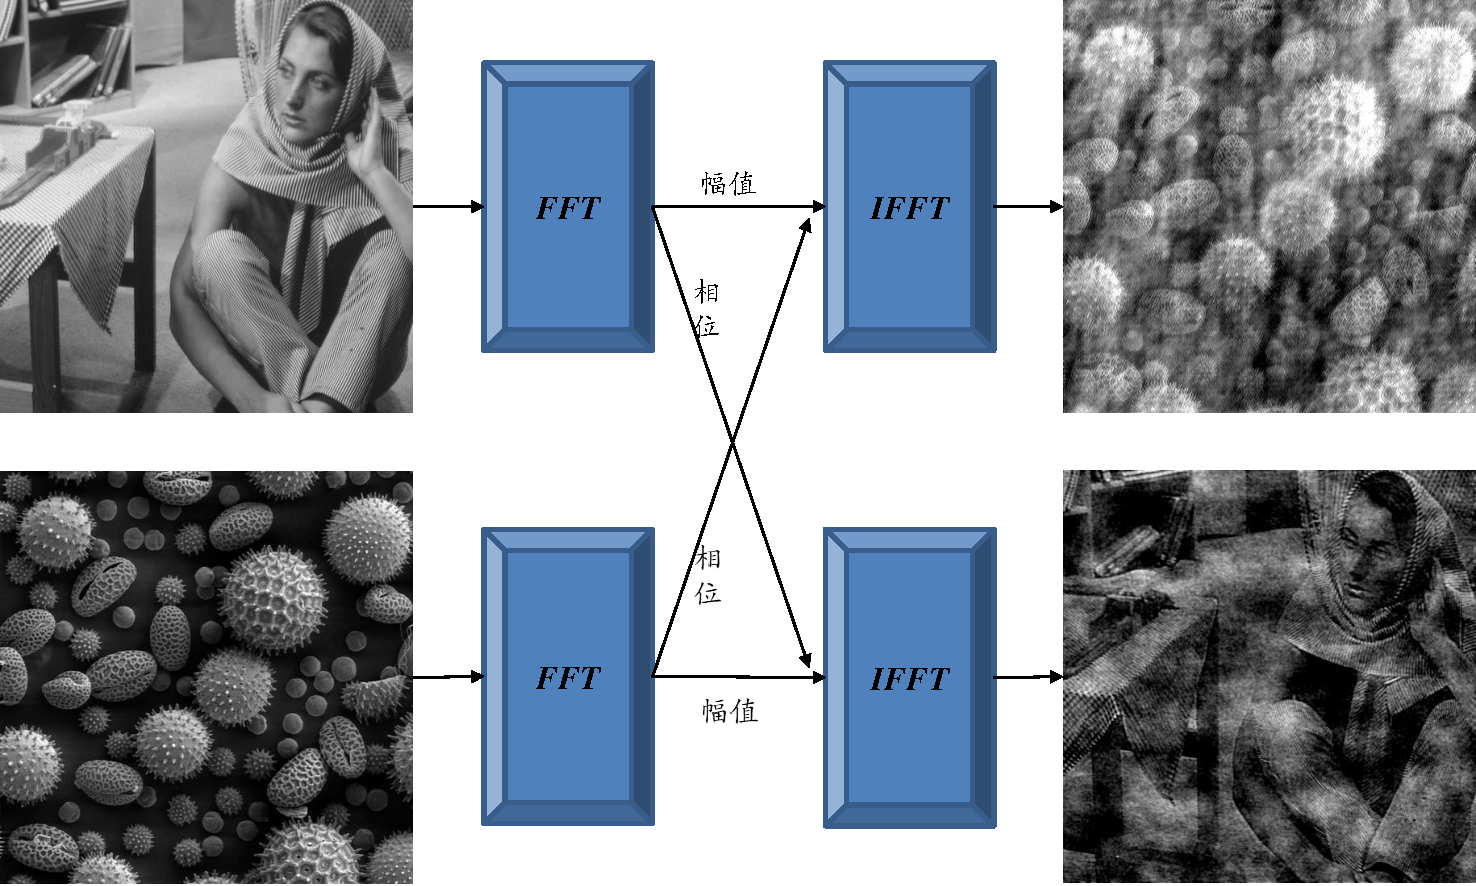
\includegraphics[width=0.8\linewidth]{1-1}
	\caption{Barbara与Pollen交换傅里叶相位后的重构示意图}\label{fig:1-1}
\end{figure}

图\ref{fig:1-1}中FFT表示傅里叶变换,IFFT表示傅里叶逆变换。从图\ref{fig:1-1}可以看出图像傅里叶变换的相位部分表征更多关于图像结构的信息。如何利用缺失相位的观测数据重构原始图像是图像重构领域的一大挑战。

站在优化的视角,相位恢复问题因非线性测量一般为非凸优化问题,其相位信息的缺失致使满足幅值非线性方程得解有无穷多个,即解空间非凸。较之凸优化问题,非凸优化问题在高维向量空间中存在多个局部候选解和鞍点,求解全局最优至少为NP(Non-deterministic Polynomial)难问题。为解决该不适定问题,现有算法通常利用图像的先验知识,包括非负性、非局部自相似性以及稀疏性等约束解空间\supercite{LiYin}。证明相位恢复算法的收敛性和收敛速度是非凸优化领域研究的难题\supercite{Hand,Jagatap,Tobias}。

深度学习在解决线性和非线性图像反问题方面取得了前所未有的成功\supercite{Ulyanov,Ulyanov,Mataev}。在图像去噪、超分辨率、图像修复、压缩感知和相位恢复等图像反问题中,基于深度卷积神经网络(Convolutional Neural Networks, CNN)的方法重构图像的质量和测试速度均优于传统的优化方法。深度生成先验已经替代了传统人工设计的图像先验,比如稀疏性,全变差,块匹配与三维滤波(Block-Matching and 3D Filtering,BM3D)、非局部自相似性等图像先验。然而深度生成先验受限于其对数据的敏感性,在面对无标签、仅有弱标签或者合成的伪标签数据时,深度生成先验的优势难以充分体现。如何将基于无监督学习的深度图像先验应用于相位恢复问题有待进一步研究。

\section{国内外研究现状}

\subsection{国内研究现状}
2012年,上海交通大学的文再文等人利用增广拉格朗日方向交替法(Augmented Lagrangian Alternating Direction Method,ADM)求解经典的图像相位恢复问题,指出了ADM算法与投影算法之间的联系,并与标准的相位恢复算法HIO(Hybrid Input-Output)、HPR(Hybrid Projection Reflection)和RAAR(Relaxed Averaged Alternating Reflection)在多幅测试图像上的性能进行比较,验证了该算法对参数的鲁棒性。

2017年,燕山大学的魏天姣等人将自然图像在梯度域下的稀疏性用于相位恢复。该算法将全变差正则项以目标函数求和的方式融合到基于支撑约束和幅值约束的相位恢复问题中,并利用ADMM算法对所提的非凸优化问题进行求解。

2018年,燕山大学的李颖等人结合图像在小波域的组稀疏性与图像在梯度域的稀疏性,面向编码衍射模型提出一种融合正交小波db10和sym4组稀疏性与全变差正则化的相位恢复算法\supercite{LiYin}。

2018年,燕山大学的石保顺等人提出了一种称为约束相位恢复的统一框架,将交替投影方法和正则化方法结合在一起。所提ConPR(Constrained Phase Retrieval)框架不仅可以从少量衍射图形中恢复高质量的图像,而且还不需要对参数进行微调。该方法将块匹配和三维滤波框架下的稀疏性纳入到所提出的ConPR框架中。优化问题由图像更新子问题和图像去噪子问题组成,之后依据数据保真项的上图概念求解数据保真项对应的优化子问题\supercite{Baoshun}。

2020年,北京理工大学的魏恺轩等人利用强化学习技术进行邻近算法迭代策略的深度展开,提出了一种免调参的即插即用邻近算法。该算法的关键部分是开发一个用于参数自动搜索的策略网络,可以通过混合无模型和基于模型的深度强化学习来有效地学习邻近算法的内部迭代参数,包括惩罚参数,降噪强度和终止时间。该算法用于解决核磁共振成像(Magnetic Resonance Imaging,MRI)和编码衍射成像问题,并且数值实验取得当前最佳(State of the Art,SOTA)的图像重构结果\supercite{Kaixuan}。

\subsection{国外研究现状}
2007年,加利福尼亚大学的Marchesini等人从交替投影策略的观点出发总结了ER、SF、HIO、DM、ASR、HPR、RAAR等算法,并应用最速下降法、共轭梯度法、最大-最小算法(Majorization Minimization,MM)求解关于衍射显微镜成像中的相位恢复问题。

2013年,斯坦福大学的Cand{\`e}s等人首次提出编码衍射模型来解决一维相位恢复问题。 Cand{\`e}s利用凸松弛技术:相位提升进行信号重构。该算法利用矩阵提升技术将相位恢复问题转化为低秩最小化问题。通过理论和实验证明它能从多个随机调制图案中准确地恢复相位信息,这些随机调制图案的采样数量为对数复杂度。但矩阵提升对于二维图像计算过于复杂,致使该算法应用受限\supercite{Candes}。

2015年,斯坦福大学的Cand{\`e}s等人提出了类似于梯度下降的WF(Wirtinger Flow)方法解决非凸形式的相位恢复问题,并以谱方法估计初始值。该算法允许从随机测量值中精确地恢复信号,具有拟线性收敛率。数值实验表明,在无噪情况下,该算法利用多个编码衍射图案能够完全重建原始图像,是近些年比较优秀的算法之一。随后,他们对WF算法进行了改进,提出了针对泊松噪声情况的TWF(Truncated Wirtinger Flow)算法。该算法在梯度计算时引入了截断机制,修正了梯度下降方向\supercite{Gross}。 

2016年,达姆施塔特工业大学的Tillmann等人提出了基于字典学习的相位恢复算法,该算法在字典未知的情况下,将待恢复图像假设为稀疏信号。在这一假设下,该算法联合重建被噪声污染的未知信号同时进行字典更新,使得估计的图像中的每一个图像块都可以被稀疏地表示。在理论上,Tillmann证明了该算法的收敛性\supercite{Tillmann}。

2018年,莱斯大学的Metzler提出prDeep算法用来解决散射介成像和转角成像中的相位恢复问题。该算法将去噪卷积神经网络DnCNN(Feed-forward Denoising Convolutional Neural Networks)嵌入RED正则化框架,利用FASTA(Fast Adaptive Shrinkage/Thresholding)算法进行求解。实验证明,该算法对泊松噪声具有鲁棒性并且能够处理各种测量矩阵模型\supercite{Metzler1}。

2019 年,美国东北大学的Hand提出了基于深度生成生先验的DPR(Deep Phase Retrieval)算法。该算法利用子梯度下降训练自编码神经网络,并依据损失函数的优化视图发现全局极小值的存在\supercite{Hand}。同年,Jagatap等人提出了基于深度图像先验(Deep Image Prior,DIP)的压缩相位恢复算法:Net-GD(Network Gradient Descent)与Net-PGD(Network Projected Gradient Descent)。数值实验结果表明,该算法在较低采样率的情况下重构图像质量优于基于稀疏先验的TVAL3、Lasso等压缩相位恢复算法。另外,在观测矩阵服从高斯分布并且满足RIP(Restricted Isometry Property)的假设下,他们证明了该算法的收敛性与最优采样复杂度的下界\supercite{Jagatap}。

\section{研究内容及结构安排}
上述国内外研究成果表明学者对实际工程应用中相位恢复算法研究的高度重视,并且取得了很多原创性成果,但也存在一些问题需要进一步攻克。本文重点研究该领域两个关键问题:散射介质成像与编码衍射成像中的相位恢复问题。散射介质成像系统如图\ref{fig:1-2}所示,相干光束照射观测目标经过空间光调制器(Spatial Light Modulator,SLM)生成衍射图案\supercite{Metzler0}。
\begin{figure}[!htbp]
	\setlength{\abovecaptionskip}{-0.02\linewidth}   
	\centering
	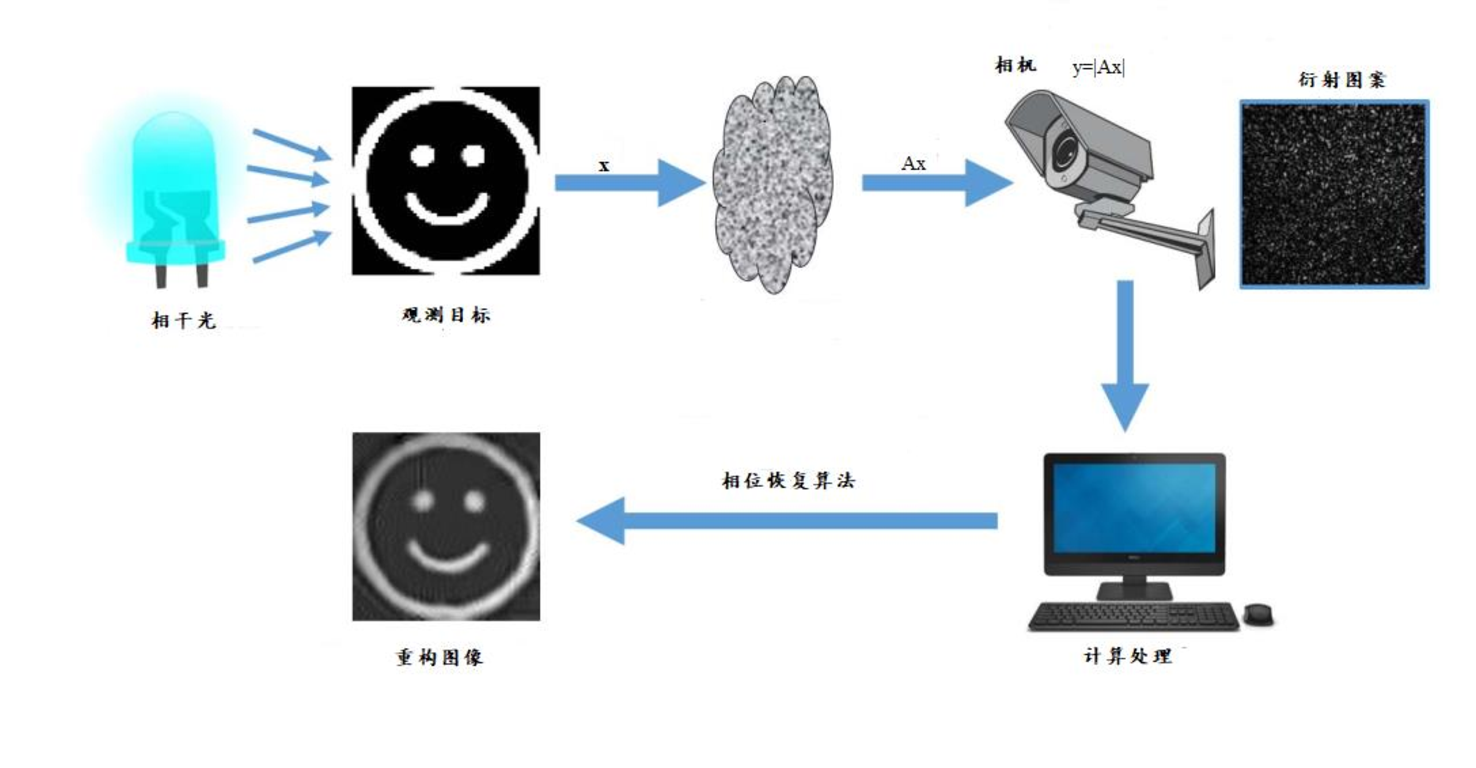
\includegraphics[width=0.8\linewidth]{1-2}
	\caption{散射介质成像装置示意图}\label{fig:1-2}
\end{figure}

编码衍射模型如图\ref{fig:1-3}所示,激光束照射待观测物体穿过相位板生成衍射图案\supercite{Candes}。二者唯一的的区别在于传输矩阵不同。为了解决上述问题,本文深入挖掘基于深度学习的去噪器和去噪正则化等高级图像先验,研究凸优化理论中的共识优化与共识方程、非凸优化理论中的基于梯度的一阶随机优化方法、基于无监督学习的深度图像先验等前沿技术构建了高效的相位恢复算法。本文主要研究内容包括如下几个方面:

(1)在编码衍射模型下,将编码衍射模型数据保真项的近邻算子与图像去噪算子作为共识方程的两个代理,提出了基于共识方程的编码衍射成像算法。在理论层面推广了文献\cite{Xiran}给出的收敛性假设条件。最后本文设计数值实验验证了该算法对含高斯和泊松噪声观测值的鲁棒性;

(2)在编码衍射模型下,依据编码衍射图案的可分离特征,提出了基于一阶随机优化的编码衍射成像算法。最后本文设计数值实验验证该算法在大规模编码衍射图案上的加速效果;

(3)在压缩相位恢复问题中,利用未训练神经网络捕获深度图像模式,并融合RED先验提出了基于深度图像先验融合RED正则项的压缩相位恢复算法。在欠采样的高斯观测矩阵下,本文设计数值实验验证该算法的重构性能以及对噪声的鲁棒性。
\begin{figure}[!hptb]  
	\centering
	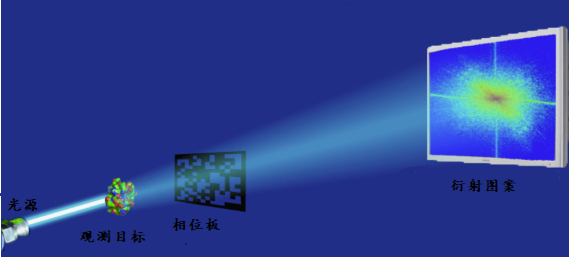
\includegraphics[width=0.6\linewidth]{1-3}
	\caption{编码衍射成像系统示意图}\label{fig:1-3}
\end{figure}

基于上述几节的研究与讨论,本文对基于非凸优化和深度学习的相位恢复算法进行了深入研究,本文的行文结构安排如下:

第\ref{chap:introduction}章,绪论。首先介绍了相位恢复问题的研究背景及其研究意义,其次总结了相位恢复的国内外研究现状,最后明确了本文的研究内容和组织结构。

第\ref{chap:theory}章,非凸优化与深度学习基本理论。首先阐述了非凸优化理论的基本问题和基本算法,其次表述了深度学习领域的基本网络架构和基于深度学习的图像去噪算法DnCNN与IRCNN(Image Restoration Convolutional Neural Networks)。

第\ref{chap:ce}章,基于共识方程的编码衍射成像算法。首先介绍了基于即插即用先验的PnP-ADMM和PnP-FBS算法以及基于RED先验的prDeep算法,其次推导了共识优化到共识方程的演化过程,最后提出了基于共识方程的编码衍射成像算法,在理论层面推广了文献\cite{Xiran}给出的收敛性假设条件。数值实验结果证明了在重构实图像时,该算法能较好的保留图像更多纹理与结构信息,具有明显的优势。

第\ref{chap:stochastic}章,基于一阶随机优化的编码衍射成像算法。首先分析了一阶随机优化算法,然后依据编码衍射图案的可分离结构提出了基于一阶随机优化的编码衍射成像法。数值实验结果表明了在编码衍射模型下,该算法可看作是第三章提出的TACE算法的加速版本,主要用于处理大规模编码衍射图案。

第\ref{chap:dip}章,基于深度图像先验融合RED正则项的压缩相位恢复算法。首先简述了深度图像先验的基本原理,然后提出了基于深度图像先验融合RED正则项的压缩相位恢复算法。该算法将显式的RED先验作为正则项添加到隐式的深度图像先验损失函数中,并利用ADMM算法进行求解。无噪与含高斯、泊松噪声的数值仿真实验证明了DPR-RED算法在欠采样率下完美重建图像的有效性以及对噪声的鲁棒性。

%第\ref{chap:chap-5}章则介绍了在文章内加入计算机程序源代码的方法。

%第\ref{chap:unit}章介绍输入数字和物理量的方法。

最后,对本文的研究工作进行了总结、归纳和分析,并指出了研究过程的不足之处,展望了下一步的研究内容。 
  % !Mode:: "TeX:UTF-8"
\chapter{非凸优化与深度学习基本理论}
\label{chap:theory}

\section{引言}
非凸优化理论在低秩矩阵分解或补全、盲反卷积、字典学习、深度学习和相位恢复领域有着广泛而深刻的应用,是国内外学者研究的热点。相较于凸优化理论中凸问题、输入样本和优化算法的完备性,非凸化理论存在诸多难题未被完美解决。但是某些非凸问题在实践应用中有着高效的求解算法和严格的收敛性分析。在非凸统计模型(包括低秩矩阵补全、盲反卷积与相位恢复)中,因为经验损失一般为非凸函数,有效的求解算法需要正则化保证梯度下降算法快速收敛。一般优化算法例如梯度下降需要合适的学习率避免迭代过程中偏离最优解,但是算法的收敛性却无法保证。非凸统计模型暗含隐式的正则化先验,此时梯度下降算法遵循隐式正则化提供的修正梯度方向收敛到与梯度随机采样机制无关的最优解邻域。神经网络的训练主要通过求解经验损失函数或结构化损失函数来完成,但这是一个困难的非线性优化问题,传统的优化理论难以直接应用。在神经网络和优化的交叉领域,长期以来研究人员积累了大量的理论研究和知识,不过这些研究或过于理论而不被大部分实践者所了解,或过于偏工程而不被理论学者所理解和欣赏。

近年来图像处理领域的研究表明,深度学习技术可以有效解决线性图像反问题,包括图像去噪、核磁共振成像和图像超分辨率。深度残差网络DnCNN与IRCNN模型学习高斯噪声分布,其去噪性能一度超越了传统的BM3D算法。上述监督学习算法需要大量的清晰图像与含噪图像对训练残差网络,基于无监督学习的深度图像先验方法利用解码-编码网络本身暗含的图像先验知识可有效去除噪声。由此表明,深度学习领域的观点和方法可迁移至解决图像处理领域,有关深度图像先验应用于非线性图像反问题中的相位恢复问题有待进学者一步研究。

\section{非凸优化的基本问题与优化算法}
优化领域最大的分野是凸与非凸,并非线性与非线性。凸优化研究在凸集上最小化凸函数的问题,大量关于凸优化的研究已经为许多类凸问题提出了有效的求解算法。因此,凸优化已经广泛地影响了科学和工程的各个学科\supercite{Stephen3}。

近年来,凸优化算法彻底改变了离散和连续优化问题的算法设计。对于子模函数最小化、整数规划和图的最大流等问题,已知的最快算法涉及到对凸优化算法的基本理论的重要应用,如梯度下降法、镜像下降法、内点方法和切割平面方法\supercite{Stephen1,Stephen2,Stephen3,Goldstein,Heide,Thomas,Chambolle1,Martin}。机器学习中的大规模优化问题对凸优化算法的需求也极大地推动了凸优化技术本身的发展。一般的凸优化问题如下所示:
\begin{equation} \label{problem:2-1}
	\begin{aligned}
		&\text{minimize}\quad f_{0}(x) \\
		&\begin{array}{@{}l@{\quad}l@{\quad}l@{}}
			\text{subject\ to}
			&f_{i}(x)\leq 0, &i=1,\ldots,m \\
			&h_{i}(x)=0, &i=1,\ldots,p \\
		\end{array}
	\end{aligned}
\end{equation}
其中$x\in\mathbb{R}^n$表示优化变量,$f_{0}(x)$表示目标函数,$f_{i}(x)\leq{0}$表示不等式约束,$h_{i}=0$表示等式约束。若$f_{0},f_{1},\ldots,f_{m}$为凸函数,$h_{i}=0$为仿射集,则式\eqref{problem:2-1}为标准的凸问题。此外,凸优化问题具有以下方面的优势:(1)凸优化问题的局部最优解就是全局最优解;(2)某些非凸问题可以通过凸松弛技术转化为凸优化问题或者近似为凸优化问题(例如拉格朗日对偶问题);(3)凸优化问题的研究较为成熟,当一个优化问题具体被归纳为一个凸优化问题时,基本可以确定该问题是可被求解的。本章基于Pytorch框架实现了凸优化算法包,其地址见\url{https://github.com/chaidisheng/Convex_Optimization}。

较之于凸优化问题,一般非凸优化问题包括三类:优化变量离散、可行集非凸或代价函数非凸\supercite{Chambolle2,Andreas,Xu,Fengmiao,PanShaohua,SunTao}。非凸优化是机器学习等领域中的基本问题,迭代优化方法缺乏理论支撑\supercite{PanShaohua, SunTao}。基于这个原因,一些学者一直致力于非凸优化理论方面的研究\supercite{SunTao,Chi,Liu,Ruoyu,Cong,Xiangyi,Danilova,Dongruo}。以下将介绍非凸优理论中基本的非凸问题与优化算法。
\subsection{主要概念}
\begin{definition} \label{def:2.1}
	凸函数:一个函数$f$被称为凸函数,如果对任意$x,y$,满足
	\begin{equation} 
		f(y)\geq{f(x)+\left\langle{\nabla f(x), y-x}\right\rangle}.
	\end{equation}
	或者对任意$x,y,0\leq\theta\leq1$,满足
	\begin{equation} 
		f(\theta x + (1-\theta)y)\leq\theta f(x)+(1-\theta)f(y).
	\end{equation}
\end{definition}

\begin{definition} \label{def:2.2}
	强凸性:一个函数$f$被称为$\mu-$强凸函数,如果对任意$x,y$,满足
	\begin{equation}
		f(y) \geq f(x)+\left\langle{\nabla f(x), y-x}\right\rangle +\frac{\mu}{2}\Vert y - x \Vert^{2}.
	\end{equation}
\end{definition}	

\begin{definition} \label{def:2.3}
	利普希茨连续性:一个函数被称为是$L_{f}$-Lipschitz,如果对任意$x,y$,满足
	\begin{equation}
		\Vert f(x) - f(y)\Vert \leq L_{f}\Vert x - y\Vert.
	\end{equation}
	另一个等价的条件为:
	\begin{equation}
		\Vert g \Vert \leq L_{f},\;g\in \partial f(x). 
	\end{equation}
\end{definition}
	
\begin{definition} \label{def:2.4}
	光滑性:一个函数$f$被称为$L_{g}$光滑(梯度是$L_{g}$-Lipschitz),如果对任意$x,y$,满足
	\begin{equation}
			\Vert  \nabla f(x) - \nabla f(y)\Vert \leq L_{g}\Vert x - y\Vert.
	\end{equation}
	或者
	\begin{equation}
		f(y) \leq f(x)+\left\langle{\nabla f(x), y-x}\right\rangle +\frac{L_{g}}{2}\Vert y - x \Vert^{2}.
	\end{equation}
\end{definition}

\begin{definition} \label{def:2.5}
	单调算子:在$\mathbb{R}^n$上的算子$F$称为单调算子,如果对$\forall(x,u),(y,v)\in{F}$,满足
	\begin{equation}
		(u-v)^\top(x-y)\geq{0}.
	\end{equation}
%	若$f(x)$为闭凸函数(Convex Closed Proper,CCP),则$F(x)=\partial{F(x)}$为最大单调算子。
\end{definition}

\subsection{基本的非凸问题}
广泛的科学与工程应用问题其本质在于求解非线性方程组\supercite{Cong}。给定观测数据$y=\left\lbrace y_{j} \right\rbrace_{1\leq j\leq m}$,它对应的非线性系统为
\begin{equation} \label{equation:2-1}
	y_{j}\approx \mathcal{A}_{j}(x),\quad 1\leq j \leq m,
\end{equation}
其中$x\in\mathbb{R}^n$表示系统输入,$\mathcal{A}_{j}$表示非线性映射。如何设计重构$x$的高效优化算法是低秩矩阵补全、相位恢复、神经网络训练等信息与统计科学领域亟待解决的难题\supercite{PanShaohua,Ruoyu,Cong,Danilova}。在合理的高斯噪声容限下,式\eqref{equation:2-1}转化为经验损失最小化问题:
\begin{equation} \label{problem:2-2}
	\mathop{\text{minimize}}\limits_{x\in\mathbb{R}^n}\quad f(x)=\sum_{j=1}^{m}|y_{j}-\mathcal{A}_{j}(x)|^{2}.
\end{equation}
一般地,优化问题\eqref{problem:2-2}非凸且属于NP难问题,难以在多项式时间复杂度内求解。工程应用中,非线性系统优化问题可用式\eqref{problem:2-2}统一表示。以下阐述几个基本的非凸优化问题:

(1)相位恢复问题:假设给定编码衍射模型传输矩阵的$m$个列向量为$\{a_j\}_{1\leq j\leq m}$,则生成编码衍射图案如下所示:
\begin{equation} \label{equation:2-2}
	y_{j}=(a_{j}^\top x)^2,\quad 1\leq  j\leq m,
\end{equation}
在方差有界的高斯噪声污染下,相位恢复对应的优化问题如下所示:
\begin{equation}\label{problem:2-3}
	\mathop{\text{minimize}}\limits_{x\in\mathbb{R}^n}\quad f(x)= \frac{1}{4m}\sum_{j=1}^{m}\big[y_{j}-(a_{j}^\top x)^2\big]^2.
\end{equation}

(2)低秩矩阵补全问题:假设给定推荐系统中对所有条目进行预测的低秩矩阵$M\in\mathbb{R}^{n\times n}$仅有限条目已知,矩阵$M$的秩远小于$n(r\ll{n})$且正定,即$M=XX^\top,X\in\mathbb{R}^{n\times r}$。低秩矩阵$M$已知的条目如下所示:
\begin{equation} \label{equation:2-3}
	Y_{j,k}=M_{j,k}=(XX^\top)_{j,k},\quad (j,k)\in{\Omega},
\end{equation}
其中子集$\Omega$的势为$m$。则$Y_{j,k}$可看作是非线性系统产生的测量值。补全低秩矩阵$M$可转化为求解如下优化问题:
\begin{equation} \label{problem:2-4}
	\mathop{\text{minimize}}\limits_{X\in\mathbb{R}^{n\times r}}\quad f(X)= \frac{n^2}{4m}\sum_{(j,k)\in\Omega}\left( Y_{j,k}-e^\top_jXX^\top e_{k} \right),
\end{equation}
其中$\{e_j\}_{1\leq j\leq m}$代表空间$\mathbb{R}^n$中的基向量。

(3)盲反卷积问题:假设给定两个信号$h,x\in\mathbb{C}^K$,相机系统仅获的$m$个双线性测量值如下所示:
\begin{equation} \label{equation:2-4}
	y_{j}=b^\mathit{H}_jhx^\mathit{H}a_{j},\quad 1\leq j\leq m,
\end{equation}
其中$a_j,b_j\in\mathbb{C}^K$是不同的卷积核,$b_j^{\mathit{H}}$为$b_j$的厄尔米特转置。重构信号$h,x$可表述为如下优化问题:
\begin{equation} \label{problem:2-5}
	\mathop{\text{minimize}}\limits_{h,x\in\mathbb{C}^K}\quad f(h,x)=\sum_{j=1}^{m}\vert y_{j}-b^\mathit{H}_jhx^\mathit{H}a_{j} \vert^2.
\end{equation}

(4)监督机器学习优化问题:假设给定$m$个训练样本$\left( x_{j}, y_{j}\right),j=1,\cdots,m$,其中$x_j\in\mathbb{R}^{dx},y_j\in\mathbb{R}^{dy}$分别代表样本点的特征向量与相应的标签向量。有监督机器学习学习任务通常是利用$x_j$的信息来预测相应的$y_j$。当我们使用一个神经网络
$f(\theta):\mathbb{R}^{dx}\to{\mathbb{R}^{dy}}$来近似$x$到$y$的映射函数时,需要选择神经网络中的参数,使得预测输出$\hat{y}_{j}=F_\theta(x_j)$最接近真实输出$y_j$。这种接近程度可以用某种距离测度进行度量。假设$\ell(\hat{y}_j,y_j)$代表$\hat{y}_j$和$y_j$之间的距离,那么优化问题表述如下所示:
\begin{equation} \label{problem:2-6}
	\mathop{\text{minimize}}\limits_{\theta}\quad f(\theta)= \frac{1}{m}\sum_{j=1}^{m}\ell(y_j,F_\theta(x_j)).
\end{equation}
寻找最优参数旨在求解非凸优化问题\eqref{problem:2-6}。在回归问题中,损失函数通常用欧氏距离的平方$\ell(y,z)=\Vert{y-z}\Vert^2$来表示,而在二分类问题中,经常选择交叉熵$\ell(y,z)=\log(1+e^{yz})$。

\subsection{基本的非凸优化算法}
高效可解释的非凸优化算法一直是学者们关注的热点,利用非凸优化方法来解决统计估计和学习问题的研究工作层出不穷。由于非凸优化算法易受虚假局部极小值的影响,传统工作通常对其持悲观看法,而简单的迭代方法,如梯度下降法,在实践中已经取得了显著的成功。然而,直到最近,这些理论基础在很大程度上一直缺乏。Yuejie Chi和Yuxin Chen等人在非凸估计的基础上开发了一个去偏估计器,使未知矩阵缺失项的置信区间能得到最优构造\supercite{Cong}。所有这些都是通过一个``一留一出”的统计分析框架实现的,该框架在处理和解耦复杂的统计依赖方面非常强大,他们将其应用于如下两个方面:(1)相位恢复问题中的随机初始化非凸方法:即使没有仔细的初始化,像梯度下降这样的简单算法也可以在对数迭代次数内找到全局最优解;(2)非凸低秩矩阵补全中的不确定性量化。本章将从如下两个方面介绍 基本的非凸优化算法。

\subsubsection{基于梯度的一阶优化算法}
梯度下降方法是优化算法中最基本的迭代方法,它用到了目标函数的梯度信息以及函数值信息,属于一阶方法。常见的梯度下降算法及其加速版本如表\ref{tab:2-1}所示。此外,基于梯度的一阶优化算法存在诸多变体,主要包括:(1)加速梯度下降法,例如共轭梯度,动量方法,Nesterov加速法;(2)梯度随机化,即每次迭代对梯度随机抽样,例如随机梯度下降(Stochastic Mini-batch Gradient Descent,SGD)、自适应梯度方法AdaGrad(Adaptive Gradient)、RMSProp(Root Mean Square Prop)、Adam(Adaptive Moment Estimation)。对于无约束优化问题\eqref{problem:2-2},当$f$光滑时,标准梯度下降方法的迭代过程为:
\begin{equation}\label{method:2-1}
	x^{k+1}:=x^k - \eta_k\nabla{f(x^k)},\quad k\geq 0.
\end{equation}
其中$\eta_k$为迭代步长或学习率。当$f$为非光滑时,次梯度的定义如下所示:
\begin{definition} \label{def:2-1}
	次梯度:向量$g$被称为一个函数$f$在$x$处的子梯度,如果对任意$y$,满足
	\begin{equation} 
		f(y) \geq f(x)+g^\top(y-x).
	\end{equation}
\end{definition}
故次梯度下降方法的迭代过程为:%\noindent 
\begin{equation}\label{method:2-2}
	x^{k+1}:=x^k-\eta_{k}g^k,\quad{k\geq{0}}.
\end{equation}
其中$g^k\in\partial{f(x^k)}$表示函数$f$的次梯度。
\begin{table}[!htbp]
	%\renewcommand{\arraystretch}{1.4}
	\def\arraystretch{1.4}\centering\zihao{5}
	\caption{基于梯度的一阶优化算法及其加速版本}\label{tab:2-1}
	\begin{tabular*}{\linewidth}{@{}@{\extracolsep{\fill}}ll@{}}
		\toprule
		算法                     & 迭代公式 \\
		\midrule
		Gradient Descent Method  & $x^{k+1}:=x^k - \eta\nabla{f(x^k)}$ \\
		Heavy-Ball Method        & $x^{k+1}:=x^k - \eta\nabla{f(x^k)} + \beta(x^k - x^{k-1})$ \\
		Nesterov's Accleerated Gradient Descent & $y^k:=x^k+\beta(x^k-x^{k-1});\,x^{k+1}:=y^k-\eta\nabla{f(y^k)}$\\
		\bottomrule
	\end{tabular*}
\end{table}

要证明一个梯度方法是收敛的,一般从以下三个方面:(1)目标函数值收敛到最优值,即$f(x^k)-f^*<\epsilon$;(2)迭代序列收敛到最优解,即$\Vert{x^k-x^*}\Vert<\epsilon$;(3)梯度趋于0,即$\Vert{\nabla{f(x^k)}}\Vert\leq \epsilon$。基于梯度的一阶优化算法及其变体的(次)线性收敛速度定义如下所示:
\begin{definition} \label{def:2-2}
	若$\exists{0 < c \leq 1}$,使迭代序列$\{x^k\}_{k\geq{0}}$满足
	\begin{equation} 
		dist(x^{k+1}, x^*)\leq(1-c){\text{dist}(x^k, x^*)},\quad \forall{k\geq{0}}
	\end{equation}
	那么,$\{x^k\}_{k\geq{0}}$具有(次)线性收敛性,其中$\text{dist}(\cdot,\cdot)$表示度量。
\end{definition}
当目标函数$f$满足不同的假设时,基于梯度的一阶算法收敛速率各不相同。收敛速度的度量如下所示:
\begin{definition} \label{def:2-3}
	若函数值序列$\{f(x^k)\}$满足
	\begin{equation}
		f(x^k)-f^*\leq{\frac{\Vert x^0 - x^* \Vert^2_2}{2\eta{k}}}.
	\end{equation}
	那么,$f(x^k)$以$\mathcal{O}(\frac{1}{k})$的速度收敛到$f^*$。
\end{definition}

定义\ref{def:2-3}的另外一种表述形式为:给定误差限$\epsilon$,令$\frac{\Vert x^0 - x^* \Vert^2_2}{2\eta{k}}\leq{\epsilon}$,则$k\geq\frac{\Vert x^0 - x^* \Vert^2_2}{2\eta{\epsilon}}$是$\mathcal{O}(\frac{1}{\epsilon})$阶的。关于基于梯度下降及其加速算法的收敛速度有如下几个结论:

(1)若$f$是$L$光滑、$\mu-$强凸函数时,当$\eta_k=\frac{1}{L}$,梯度下降法(Gradient Descent)的收敛速度为:
\begin{equation}
	f(x^k)-f^*\leq{\mathcal{O}((1-\frac{\mu}{L})^k)}.
\end{equation}即$\mathcal{O}(\log{\frac{1}{\epsilon}})$阶;
当$\eta=\frac{4}{\sqrt{L}+\sqrt{\mu}}$,$\beta=\frac{(\sqrt{L}-\sqrt{\mu})^2}{(\sqrt{L}+\sqrt{\mu})^2}$时,重球法(Heavy-Ball Method)的收敛速度为:
\begin{equation}
	f(x^k)-f^*\leq{\mathcal{O}((1-\sqrt{\frac{\mu}{L}})^k)}.
\end{equation}即$\mathcal{O}(\log{\frac{1}{\epsilon}})$阶,此时目标函数$f$二次连续可微;
当$\eta=\frac{1}{L}$,$\beta=\frac{\sqrt{L}-\sqrt{\mu}}{\sqrt{L}+\sqrt{\mu}}$时,Nesterov加速算法(Nesterov's Accleerated Gradient Descent)的收敛速度为:
\begin{equation}
	f(x^k)-f^*\leq{\mathcal{O}((1-\sqrt{\frac{\mu}{L}})^k)}.
\end{equation}即$\mathcal{O}(\log{\frac{1}{\epsilon}})$阶,此时目标函数$f$不需要二次连续可微。

(2)若$f$是$L$光滑、凸函数时,当$\eta=\frac{1}{L}$,$\beta_k=\frac{\theta_k(1-\theta_{k-1})}{\theta_{k-1}}$,其中$\theta^2_k=(1-\theta_k)\theta_{k-1}^2$,$\theta_0=1$时,Nesterov加速算法的收敛速度为:
\begin{equation}
	f(x^k)-f^*\leq{\mathcal{O}(\frac{1}{k^2})}.
\end{equation}收敛阶为$\mathcal{O}(\frac{1}{\sqrt{\epsilon}})$。而一般梯度算法的收敛阶为$\mathcal{O}(\frac{1}{\epsilon})$。

在深度学习中,神经网络的训练问题\eqref{problem:2-6}可用重新表述为如下优化问题:
\begin{equation} \label{problem:2-7}
	\mathop{minimize}\limits_{\theta}\quad f(\theta)=\frac{1}{B}\sum_{i=1}^{B}f_i(\theta).
\end{equation}
其中$f_i(\theta)$是训练集中一组小批样本(mini-bach)的损失函数之和,$B$为小批样本的总数($m$为总样本数)。$f_i(\theta)$的具体形式已知,只需计算其梯度即可。随机梯度下降的工作原理如下:在第$k+1$次迭代中,随机选择一组小批样本的梯度进行更新:
\begin{equation} \label{method:2-3}
	\theta^{k+1}:=\theta^k-\eta_k\nabla{f_i(\theta^k)}.
\end{equation}
其中$\theta_k$代表步长(学习率)。学习率的选取有如下策略:(1)步长恒定,这种随机梯度下降法也被称为自然梯度下降(Vanilla SGD);(2)非恒定步长,例如,学习率的热启动技术(在多次迭代中先使用非常小的学习速率,然后增加到常规学习速率)被广泛使用深度学习中;(3)循环学习率,基本思想是让步长在下限和上限之间跳跃。研究理论分析表明,神经网络优化具有特殊的结构,因此经典优化理论可能不适用于神经网络。梯度下降的收敛加速问题也是理论研究的重点。固定学习率与递减学习率的比较与分析一直是SGD的理论分析的重点。相关实验证明,SGD相对于普通梯度下降的收敛速度有所加快,但这种加速效果也取决于许多其他因素。

带动量的SGD算法在第$k+1$次迭代中,随机选取小批样本,并通过以下方式更新动量项和参数:
\begin{equation} \label{method:2-4}
	\begin{aligned}
		m^k&:=\beta{m^{k-1}} + (1-\beta)\nabla{f_i(\theta^k)}\\
		\theta^{k+1}&:=\theta^k-\eta_{k}{m^k}.
	\end{aligned}
\end{equation}
其中$\beta$为动量参数。上述方法广泛应用于机器学习领域,它们在实际应用中的收敛速度比一般的随机梯度法要快,而且在处理凸问题或二次问题中也具有理论上的优势。带动量的SGD的优异表现仅适用于批处理方法。但在具体的实践应用中,该算法的理论分析几乎无法实现。存在两个方案可以加速SGD算法:其一,通过利用诸如方差缩减之类的技巧,更高级的优化方法来实现动量与SGD这一组合在收敛速度上的理论提升。但这些方法有些复杂, 在实践中并不流行。其二,通过考虑问题的更多结构和更简单的SGD变体来实现加速。上述方法仅适用于凸问题,因此不能直接适用于非凸的神经网络问题。最近,方法二有许多理论性新方法的设计,使其收敛速度在一般非凸问题上比一般的随机梯度下降还要快,但这些方法尚待广泛地应用与时间的检验。

第三类流行的方法是如AdaBelief、AdaGrad、RMSProp和Adam的自适应梯度下降\supercite{Liu,Xiangyi}。AdaGrad的描述如下:在第次迭代中,随机选择小批量样本并将参数更新为:
\begin{equation} \label{method:2-5}
	\theta^{k+1}:=\theta^k\eta_k\nu_k^{-1/2}\circ{g^k}.
\end{equation}
其中$g^k=\nabla{f_i(\theta^k)}$,$\nu_k=\sum_{i=1}^{T}g_i\circ{g_i}$,$\circ$表示哈达玛积(Hadamard Product)。AdaGrad的一个缺点是它对所有过去的梯度都一视同仁,因此对过去的梯度使用指数递减权重。$\nu_k$的这一新定义启发了RMSProp和一个更复杂的算法AdaDelta(Adaptive Learning Rate Method)。AdaGrad自适应梯度方法是用来处理稀疏和高度不平衡的数据,也被普遍认为比普通的SGD和带动量的SGD有更快的收敛速度但更差的泛化性。对于生成对抗网络这类的复杂情况,通常默认使用自适应方法,因为其具有稳定性\supercite{Ruoyu,Dongruo,Xiangyi}。

最新提出的AdaBelief(Adapting Stepsizes by the Belief in Observed Gradients)考虑了损失函数的曲率、分母中梯度的符号。在方差较小时,Adam中的更新方向接近于符号下降偏离了真正的梯度方向,符号更新效应可能导致自适应方法和SGD之间的泛化差距\supercite{Dongruo}。但在AdaBelief中,当$g_t$的方差对于所有坐标都相同时,更新方向会与梯度方向匹配。当方差不均匀时,AdaBelief会在方差大时采取小步长。研究者通过实验验证了AdaBelief在图像分类和语言建模方面快速收敛与准确度高的优势。


\subsubsection{凸和非凸ADMM算法}
本节将介绍ADMM、线性ADMM及其相关变体BADMM(Bregman ADMM)算法;(2)最近凸和非凸ADMM算法收敛性分析的最新成果。

一般带有线性约束的复合优化问题在不同的学科和应用中无处不在,例如机器学习与图像反问题中的正则化模型,其优化问题可以写为:
\begin{equation}\label{problem:2-8}
	\begin{aligned}
		&\text{minimize}\quad f(x)+g(z)\\
		&\text{subject\ to}\quad Ax + Bz = c
	\end{aligned}
\end{equation}
其中$f$和$g$是闭函数但可能非凸,并且$x\in\mathbb{R}^n$,$z\in\mathbb{R}^m$,$A\in\mathbb{R}^{pxn}$,$B\in\mathbb{R}^{pxm}$,$c\in\mathbb{R}^p$。解决该问题经典有效的算法是交替方向乘子法。ADMM实际上研究的是问题\eqref{problem:2-8}的增广拉格朗日问题而不是原始问题\eqref{problem:2-8}。其增广拉格朗日问题为:
\begin{equation}\label{equation:2-5}
	L_\rho(x,z,y)=f(x)+g(z)+y^{\top}(Ax+Bz-c)+(\rho/2)\Vert{Ax+Bz-c}\Vert_2^2.
\end{equation}
其中$\rho>0$是惩罚参数。在每次迭代中,ADMM算法以交替的方式运行:每次它仅极小化一个变量并保持其他变量不变;而拉格朗日乘子变量$y$由反馈策略(对偶上升)更新。ADMM的迭代格式可以写为:
\begin{equation}\label{method:2-6}
	\begin{cases}
		x^{k+1}:=\arg\min_{x}{L_{\rho}(x,z^k,y^k)} \\
		z^{k+1}:=\arg\min_{z}{L_{\rho}(x^{k+1},z,y^k)} \\
		y^{k+1}:= y^k+\rho{(Ax^{k+1}+Bz^{k+1}-c)}
	\end{cases}
\end{equation}
令$u=(1/\rho)y$,则式\eqref{method:2-6}可写为:
\begin{equation}\label{method:2-7}
	\begin{cases}
		x^{k+1}:=\arg\min_{x}\left({f(x)+(\rho/2)\Vert{Ax+Bz^k-c+u^k}\Vert^2_2}\right) \\
		z^{k+1}:=\arg\min_{z}\left({g(z)+(\rho/2)\Vert{Ax^{k+1}+Bz-c+u^k}\Vert^2_2}\right) \\
		u^{k+1}:=u^k+(Ax^{k+1}+Bz^{k+1}-c)
	\end{cases}
\end{equation}

\begin{definition}\label{def:2-4}
	函数$f$的近邻算子$\text{prox}_{\lambda{f}}:\mathbb{R}^n\to\mathbb{R}^n$
	\begin{equation}\label{proximal-operator}
		\begin{aligned}
			\text{prox}_{\lambda f}(v)\overset{\underset{\mathrm{def}}{}}{=}\arg\min_{x}\left({\lambda f(x)+\frac{1}{2}||x-v||_2^2}\right).
		\end{aligned}
	\end{equation} 
\end{definition}

\begin{definition} \label{def:2-5}
	函数$f$的广义近邻算子$\text{prox}_{\lambda{f}}:\mathbb{R}^n\to\mathbb{R}^n$
	\begin{equation}\label{generalized-proximal-operator}
		\begin{aligned}
			\text{prox}_{\lambda f}(v,\Gamma)\overset{\underset{\mathrm{def}}{}}{=}\arg\min_{x}\left({\lambda f(x)+\frac{1}{2}||x-v||_{\Gamma^{-1}}^2}\right).
		\end{aligned}
	\end{equation}
	其中$\Gamma$为半定矩阵。
\end{definition}

另外,稀疏性问题极大促进了ADMM的发展。在这些问题中,其中一个目标函数的近端映射很容易计算;而另一个目标函数可以非常快速地更新每次迭代。但是在一般的ADMM中,变量$x$和$y$由矩阵$A$和$B$耦合,这导致当$A$为非单位矩阵或循环矩阵时使用近端映射计算量很大。因此,文章提出线性化的ADMM,其采用线性化技术用于增广拉格朗日函数中的二次项。线性ADMM对应的迭代格式为:
\begin{equation}\label{method:2-8}
	\begin{cases}
		x^{k+1}:=\text{prox}_{\mu{f}}(x^k−(\lambda/\rho)A^\top(Ax^k+Bz^k+u^k-c)) \\
		z^{k+1}:=\text{prox}_{\gamma{g}}(z^k−(\gamma/\rho)B^\top(Ax^k +Bz^k+u^k-c)) \\
		u^{k+1}:=u^k+(Ax^{k+1}+Bz^{k+1}-c)
	\end{cases}
\end{equation}

Bregman距离可以被视为欧氏距离平方的延伸,它广泛应用于图像处理和机器学习中的各种模型和算法,其定义如下:
\begin{definition}\label{def:2-6}
	给定可微函数$\phi,x,y\in{dom(\phi)}$之间的Bregamn距离定义为
	\begin{equation}
		B_{\phi}(x,y)\overset{\underset{\mathrm{def}}{}}{=}\phi(x)-\phi(y)-\left<\nabla\phi(y),x-y\right>,
	\end{equation}
	如果$\phi=x^\top{M}x$,其中$M$半定矩阵,那么$B_\phi(x,y)=\Vert{M^{\frac{1}{2}}(x-y)}\Vert^2_2=(x-y)^\top{M(x-y)}$。
\end{definition}
基于Bregman距离提出更为一般的ADMM,可以表示为:
\begin{equation}\label{method:2-9}
	\begin{cases}
		x^{k+1}:=\arg\min_{x}{L_{\rho}(x,z^k,y^k)+B_\phi(x,x^k)} \\
		z^{k+1}:=\arg\min_{z}{L_{\rho}(x^{k+1},z,y^k)+B_\psi{(z,z^k)}} \\
		y^{k+1}:=y^k+\rho{(Ax^{k+1}+Bz^{k+1}-c)}
	\end{cases}
\end{equation}
其中$B_\psi(y,y^k)$和$B_\phi(x,x^k)$是Bregman距离,可以看到BADMM包含许多正则化和线性化ADMM的算法。在图像反问题与机器学习正则化模型中,若令$A=I_n,B=-I_n,c=\vec{0}$,则线性ADMM方法\eqref{method:2-8}退化为:
\begin{equation}\label{method:2-10}
	\begin{cases}
		x^{k+1}:=\text{prox}_{f/\rho}(z^k − u^k) \\
		z^{k+1}:=\text{prox}_{g/\rho}(x^{k+1} + u^k) \\
		u^{k+1}:=u^k+(x^{k+1}-z^{k+1})
	\end{cases}
\end{equation}

关于ADMM算法的收敛性分析有如下几个结论:(2)凸优化理论的先驱Boyd在$f,g$为闭凸函数(closed,proper,convex)且增广拉格朗日函数$L_0$存在鞍点的情况下,证明了ADMM的收敛性,以及给出了原始与对偶停止迭代误差\supercite{Stephen1};(2)Zheng Xu等人提出了基于自适应松弛技术的ADMM算法(Adaptive Relaxed ADMM,ARADMM),之后在自适应罚参数与松弛因子特定选取下利用变分不等式证明了该算法的收敛性\supercite{Xu};(3)孙涛等人提出了一般的ADMM收敛性分析统一框架。在此框架下,很多现有的ADMM收敛性分析可以归纳进该框架。另外,根据统一框架还能够设计出针对结构非凸优化问题的ADMM算法:一个是针对泛$\ell_q$正则化约束优化问题,另一个是针对$\ell_{1-2}$正则化约束优化,同时孙涛给出了两种非凸ADMM算法的收敛性分析\supercite{SunTao}。

\section{深度学习基本原理与图像去噪应用}
近年来,深度学习技术得到了快速的发展,并广泛应用于图像处理领域。相对于传统图像处理算法,深度学习技术从海量的训练数据中学习到的先验知识具有更强的泛化能力和更复杂的参数化表达,且无需调节算法参数以适应不同的应用场景。如何利用深度学习算法提升图像处理的性能也变成了一个重要的研究方向。

尽管深度学习显著促进了图像处理领域的发展,但是受限于其对训练数据的敏感性,在面对无标签、仅有弱标签或者合成伪标签的数据时,深度学习技术的优势难以充分体现。而基于无监督学习的深度图像先验方法为解决上述难题提供了思路:生成器网络的结构足以在任何学习之前捕获大量的低级图像统计信息。

\subsection{深度卷积神经网络}
深度卷积神经网络(CNN)是一种有效的特殊神经网络,目前在各种竞赛基准上取得了最优结果\supercite{Alex,Simonyan,Kaiming,Ronneberger}。深度卷积神经网络主要通过使用多个非线性特征提取阶段实现超强的学习能力,这些阶段能够从数据中自动地学习分层表示。大量标注数据及GPU硬件结构的改进加速了卷积神经网络的研究,致使新的深度卷积神经网络架构层出 不穷。最近,Kaggle比赛表明,创新的架构理念以及超参数优化可以提高卷积神经网络在各种视觉相关任务上的性能。鉴于此,关于卷积神经网络设计的不同想法被提出,如使用不同的激活函数、损失函数、参数优化、正则化以及重构处理单元。然而,在表征能力方面的主要改进是通过重构处理单元来实现的。尤其是,使用块而不是层作为结构单元的想法获得了极大关注\supercite{GeDaohui}。

经典的卷积神经网络架构通常包含池化层与卷积层的交替,最后一层是全连接层与Softmax层的组合。在特定应用中,全连接层替换为平均池化或最大池化层。除了基本的学习单元外,还结合了其他正则化技术,例如批次归一化或Dropout,以优化深度卷积神经网络的性能。另外,卷积神经网络组件的自动搜索技术(Neural Architecture Search,NAS)在设计新体系架构和获得增强性能方面起着举足轻重的作用。本节简要讨论了这些组件在CNN体系结构中的作用以及经典的深度卷积神经网络架构。
\subsubsection{深度卷积神经网络基本组件}
卷积层通过将图像划分成感受野与一组特定的权重进行卷积(自相关)来工作。卷积运算表示如下:
\begin{equation} \label{conv}
	F_l^k=(I_{x,y}\ast{K_l^{k}}).
\end{equation}
其中$I_{(x,y)}$表示输入图像,$x,y$表示具体位置,$K_l^k$表示第$k$层的第$l$个卷积核。卷积层对输入图像的小部分区域提取局部相关的像素值特征生成特征图。经过卷积层产生的特征图可能出现在图像的不同位置。特征一旦提取后,只要保留相对于其他特征的近似位置,其精确位置就不再重要。利用卷积进行池化或下采样的局部操作,汇集了感受野附近的相似信息,并在该局部区域内输出特征图。池化操作如下表示:
\begin{equation} \label{pool}
	Z_l=f_p({F_{x,y}^l}).
\end{equation}
其中$Z_l$表示第$l$个输出特征图,$F_{x,y}^l$表示第$l$个输入特征图,而$f_p(\cdot)$定义了池化操作的类型。池化操作不仅有助于提取具有平移不变性的组合特征,而且将特征图的尺寸减小至不变的特征集有利于调节网络的复杂性以及减小过拟合的风险。卷积神经网络中使用了不同类型的池化公式,包括最大池化、平均池化、空间金字塔合并等。

激活函数的非线性有助于学习目标的复杂模式,选择适当的激活函数可提升模型的性能。不同类型的激活函数如图\ref{fig:2-1}所示。
\begin{figure}[!htbp]
	\centering
	\subfigure[Sigmod型激活函数]{
		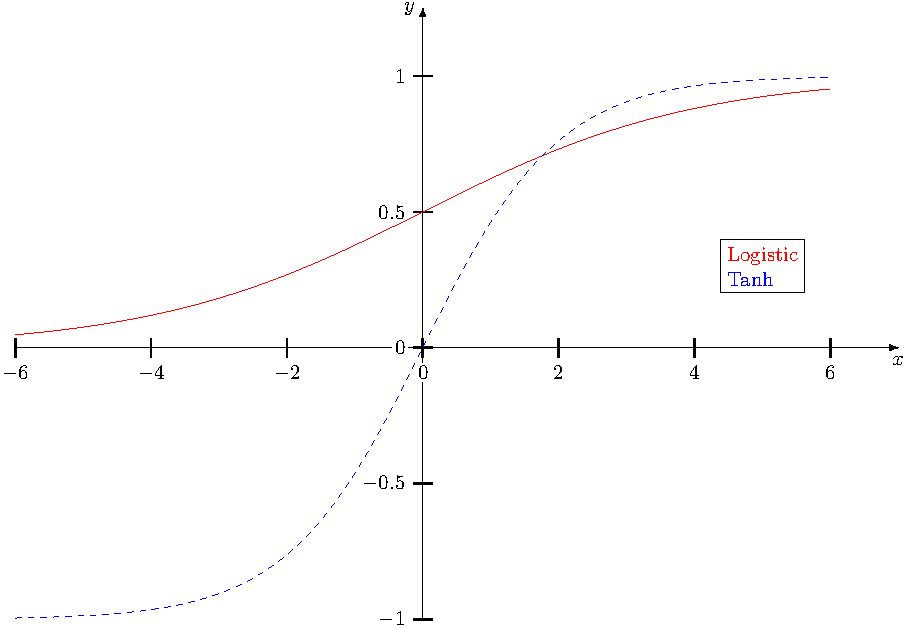
\includegraphics[width=0.4\linewidth]{2-1-1}
	}\hspace{0.1\linewidth}
	\subfigure[ReLU激活函数及其变体]{
		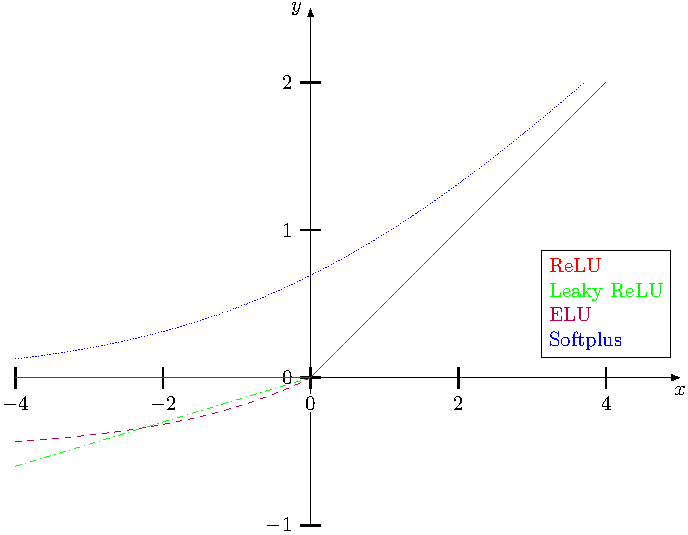
\includegraphics[width=0.4\linewidth]{2-1-2}
	}
	\caption{激活函数示意图} \label{fig:2-1} 
\end{figure}

图\ref{fig:2-1}中激活函数包括sigmoid、tanh、maxout、ReLU及其变体,例如leaky ReLU、ELU和PReLU等。输入卷积特征图的激活函数如下所示:
\begin{equation} \label{activation}
	T_l^k=f_A(F_l^k).
\end{equation}
其中$F_l^k$是卷积运算的输出,它通过激活函数$f_A(\cdot)$返回第$k$层的转换输出$T_l^k$。不同的激活函数用于引入特征的非线性组合。另外,ReLU及其变体的梯度有界,可以克服神经网络训练过程中梯度消失的问题。

批次归一化(Batch Normalization,BN)的提出是为了解决神经网络各层输出特征图内部协方差平移(Internal Covariate Shift,ICS)相关的问题。ICS偏移量导致各层输入分布与输出分布不一致,这会降低模型训练的收敛速度(通过将学习率强制为较小值来解决),并对参数初始化要求高。对变换后的特征图$T_l^k$执行批次归一化如下所示:
\begin{equation} \label{bn}
	N_l^k=\frac{F_l^k-\mu_B}{\sqrt{\sigma_B^2+\epsilon}}.
\end{equation}
其中$N_l^k$表示归一化特征图,$F_l^k$表示输入特征图,$\mu_B$和$\sigma_B^2$分别表示小批次特征图的均值和方差。批次归一化通过将特征图设为零均值和单位方差来统一其分布。此外,批次归一化可以平滑梯度流并充当调节因素,从而提高网络的泛化性。

Dropout引入了网络内部的正则化,在训练过程中它通过以一定概率丢弃神经元的方式提高网络的泛化性。在神经网络中,学习某个非线性组合会相互适应导致其过拟合。某些连接单元的这种随机丢弃会产生几种稀疏的网络体系结构,之后选择一个权重较小的代表性网络,将这种选择的架构视为所有提出网络的近似。

\subsubsection{深度卷积神经网络主要架构}
随着CNN成功应用于图像识别领域,Simonyan等人提出了模块化的分层结构体系VGG-19,如图\ref{fig:2-2}所示。与AlexNet相比,VGG的深度为$19$层,以模拟深度与网络表示能力的关系。VGG用一堆小尺寸的$3x3$卷积层代替了$5\times5$和$11\times11$卷积层,并通过实验证明,同时放置$3x3$卷积核可以达到大尺寸卷积核的效果。小尺寸卷积核的另一个好处是通过减少参数的数量降低了网络的计算复杂性。这些发现为在神经网络中使用较小尺寸的卷积核创造了新的研究趋势。虽然VGG未在2014年的ILSVRC竞赛中名列前茅,但由于其简单、同质的拓扑结构和增加的深度而闻名。VGG的不足之处主要在于计算成本高。即使使用小尺寸的卷积核,仍有约$1.4$亿个参数。
\begin{figure}[!hptb]
	\centering
	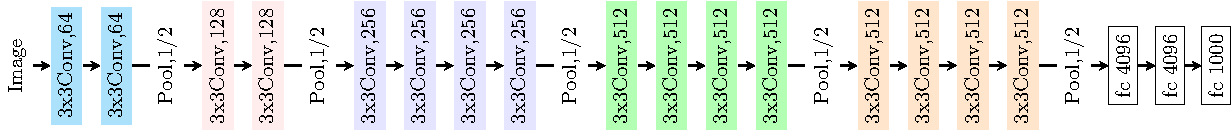
\includegraphics[width=\linewidth]{2-2}
	\caption{VGG16网络架构示意图}\label{fig:2-2}
\end{figure}

GoogleNet赢得了2014年ILSVRC竞赛的冠军,亦称为Inception-V1。GoogleNet体系结构的主要目标是在降低计算成本的同时实现高精度。它在卷积神经网络中引入了inception块的新概念,通过拆分、变换和合并的思想整合了多尺度卷积层。inception块的体系结构如图\ref{fig:2-3}所示。该模块封装了不同大小的卷积核($1\times1$、$3\times3$和$5\times5$),以捕获不同尺度(细粒度和粗粒度)的空间信息。GoogleNet有助于解决学习同一图像类别中存在的各种类型变体有关的问题。除了提高学习能力外,GoogleNet的优点还在于提高了CNN参数的利用率,以及应用批次归一化技术与RMSProp优化器加速其训练的过程。但是,GoogleNet的主要缺点是其异构拓扑结构需要在模块之间进行自定义。此外,GoogleNet的另一个限制是表示瓶颈,它极大地减少了下一层的特征空间,因此有时可能会导致有用信息的丢失。
\begin{figure}[!hptb]
	\centering
	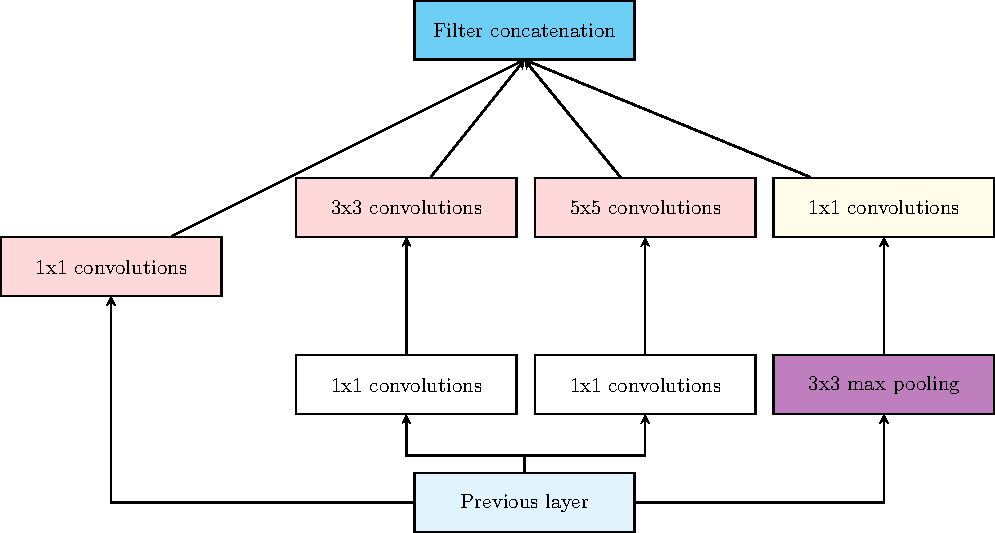
\includegraphics[width={0.8\linewidth}]{2-3}
	\caption{Inception块基本结构示意图}\label{fig:2-3}
\end{figure}

ResNet由He等人提出,被认为是深度网络的延续,其网络架构如图\ref{fig:2-4}所示。ResNet通过在卷积神经网络中引入残差学习的概念彻底改变了卷积神经网络架构,解决了神经网络训练过程中的退化问题。神经网络层数的加深致使神经网络参数空间变得复杂,因此提升了优化的难度。ResNet的残差结构有效降低了学习的难度,解决了深层神经网络的性能退化问题。
\begin{figure}[!hptb]
	\centering
	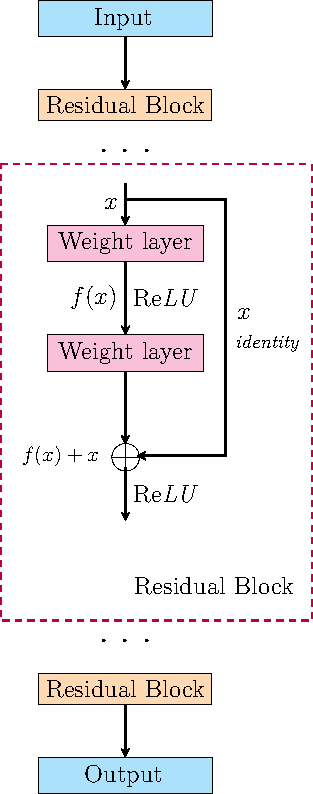
\includegraphics[height={0.6\linewidth}, width={0.3\linewidth}]{2-4}
	\caption{ResNet网络架构示意图}\label{fig:2-4}
\end{figure}

生成对抗网络(Generative Adversarial Networks,GAN)是Goodfellow等人开创性提出的一种生成式模型,其结构如图\ref{fig:2-5}所示。GAN一般由两个网络组成:生成器(Generator)和鉴别器(Discriminator)。其次,GAN是一种以半监督方式训练分类器的方法,用于解决带标签训练集样本少的问题。GAN模型训练时不像VAE一样需要对隐变量做出分布假设,生成器的参数更新不是直接来自数据样本,而是来自判别器提供的梯度信息。GAN本质上用判别器去学习损失函数,而非直接优化生成样本与标签的距离。
\begin{figure}[!htbp]
	\centering
	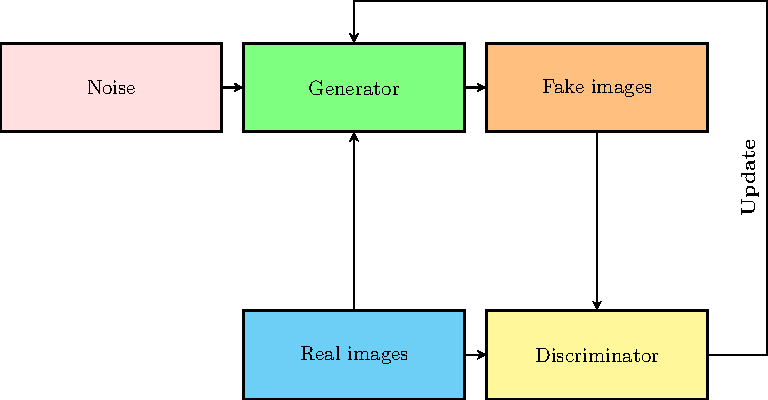
\includegraphics[width={0.8\linewidth}]{2-5}
	\caption{GAN网络架构示意图}\label{fig:2-5}
\end{figure}

GAN的学习优化过程就是一个极小极大博弈(Min-Max Game,MMG)问题,目的是寻找二者之间的一个纳什均衡,使生成器估计数据样本的真实分布。GAN的损失函数如下所示:
\begin{equation} \label{second:GAN}
	\min_{G}\max_{D}\quad V(D,G)=\mathbb{E}_{x\sim{p_{data}(x)}}[\log{D(x)}]+\mathbb{E}_{z\sim{p_{z}(z)}}[\log{(1-D(G(z)))}].
\end{equation}
在生成对抗网络中,如果没有对辨别器进行约束,那么其产生的梯度通常并不具有充分的信息来引导生成器进行更新,最新的解决方案是对判别器利用实谱归一化技术进行利普希茨约束。同时GAN生成的样本虽然具有多样性,但是存在模式崩溃与模式单一的现象。

U-Net由Ronneberger等人在Kaggle挑战赛上提出,它应用于医疗影像分割任务。U-Net是典型的Encoder-Decoder结构,Encoder进行特征提取,Decoder进行解码操作,如图\ref{fig:2-6}所示。
\begin{figure}[!htbp]
	\centering
	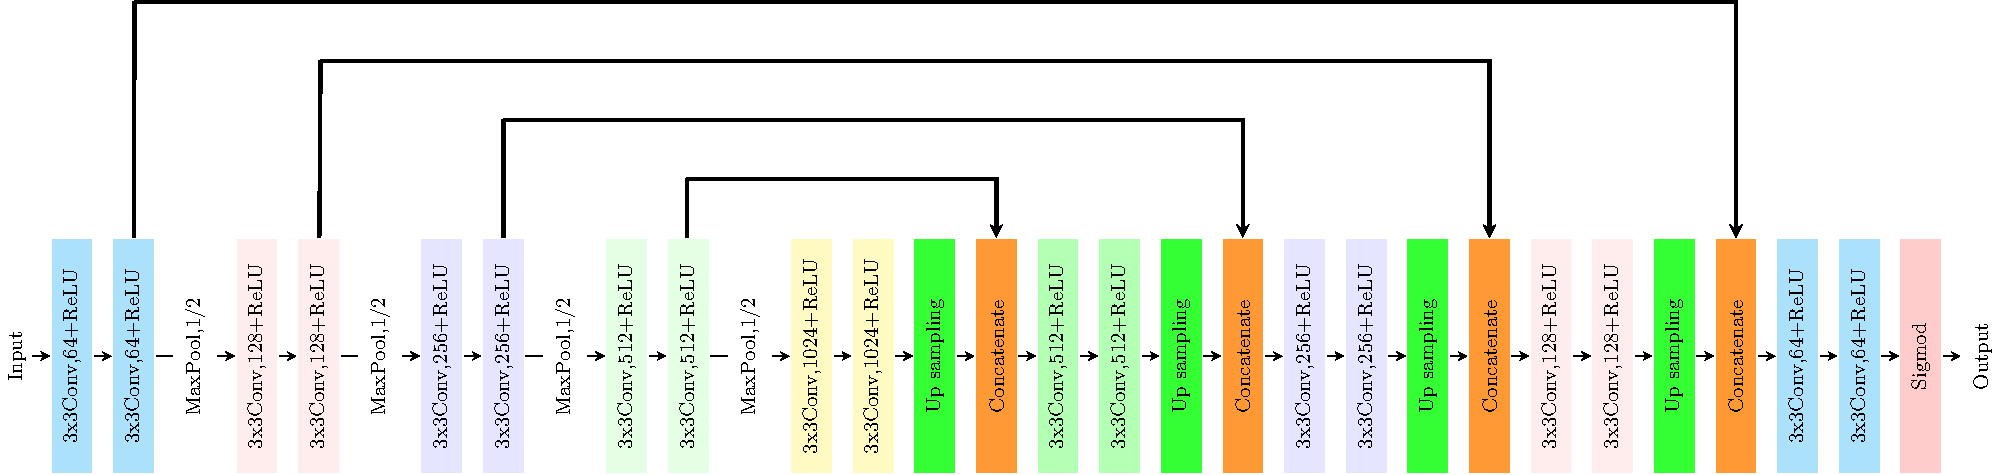
\includegraphics[width={\linewidth}]{2-6}
	\caption{U-net网络架构示意图}\label{fig:2-6}
\end{figure}

U-Net网络架构中一个重要的组成部分是在上采样中拼接了来自编码网络大量的浅层特征图,这些通道允许网络将上下文信息传播到具有更高分辨率的层。因此,拓展路径或多或少地与收缩路径对称,并产生一个U形结构。U-Net可以提取图像不同区域不同尺度的特征,这对像处理来说具有天然的优势。最近,U-Net结合循环神经网络(Recurrent Neural Network,RNN)、残差结构、注意力机制设计出R2U-Net、Deep Residual U-Net、Attention U-Net等语义分割网络,为自动驾驶、自动扣图等领域开辟出新的研究途径。

\subsection{基于深度学习的图像去噪算法}
深度学习技术在图像降噪方面获得了极大的成功。但是,处理不同类型噪声的学习方法存在较大的差异。具体来说,基于深度学习的方法可以有效估计真实的噪声分布\supercite{Chunwei}。但是,迄今为止很少有相关研究来总结用于图像去噪的不同深度学习技术。本节介绍了图像去噪领域内两种典型的深度学习去噪器DnCNN和IRCNN。

图像去噪任务要求在尽可能去除噪声的同时,还应保持图像的边缘、纹理等结构信息。再者,对于普遍存在的图像模糊问题,如何有效估计模糊过程、处理噪声和估计误差等,将对恢复高质量、清晰的图像至关重要。图像去噪任务的观测模型如下所示:
\begin{equation} \label{equation:2-6}
	y = x + v.
\end{equation}
其中$x,y,v$分别代表干净图像、噪声图像和高斯噪声(AWGN)。下面介绍两种经典的深度学习去噪模型:

(1)DnCNN由张凯等人提出,其网络架构如图\ref{fig:2-7}所示\supercite{Kai}。DnCNN采用残差学习训练残差映射$R(y)\approx{v}$,然后得到干净图像$x=y-R(y)$。DnCNN模型有两个主要特征:采用残差学习来学习$R(y)$,并结合BN层来加速训练过程;卷积与ReLU结合,DnCNN通过隐层逐渐将图像结构与噪声干扰分开。这种机制类似于EPLL和WNNM等方法中采用的迭代噪声消除策略,但DnCNN以端到端的方式进行训练。对于某一个特定的噪声水平,DnCNN可以在视觉效果和数值上达到当前SOTA的水平。再者,DnCNN可以扩展通用的降噪任务,即训练一个去盲高斯噪声的DnCNN模型可优于针对某种具体噪声水平的方法。同样的方法可以扩展到一般的降噪任务,例如单幅图像超分率和jpeg去块任务。
\begin{figure}[!htbp]
	\centering
	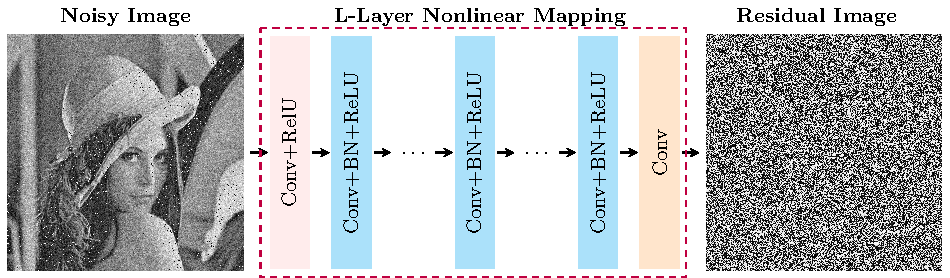
\includegraphics[width=\linewidth]{2-7}
	\caption{DnCNN网络架构示意图}\label{fig:2-7}
\end{figure}

(2)IRCNN同样由张凯等人提出,作为图像先验应用于去模糊、单幅图像超分辨率等图像反问题。其网络架构如图\ref{fig:2-8}所示\supercite{ZhangKai}。IRCNN使用空洞卷积扩大感受野以捕获更多的上下文信息。另外,空洞卷积不仅可以提高性能和效率,还能挖掘更多图像的边缘模式。在图像去噪任务中,背景信息对重构受损像素具有很大的作用。

一般用于扩大卷积神经网络感受野的方法为:一是增大卷积核尺寸;二是加深卷积深度。因此,最佳的设计是在现有卷积神经网络的结构体系之上,使用深度更深的$3\times3$卷积核。另外,扩张卷积以其扩大感受野的能力而闻名,同时保持传统$3\times3$卷积的优点。具有膨胀因子$s$的扩张卷积可简单地解释为大小为$(2s+1)\times(2s+1)$的稀疏滤波器,其中只有$9$个固定位置可以为非零数。因此,IRCNN每层的等效感受野是$3,5,7,9,7,5,3$,此时$L=7$,IRCNN网络的感受野是$33\times33$。如果使用传统的$3\times3$卷积核,网络感受野大小为$15\times15$或者具有相同感受野但深度为$16$。再者,DnCNN与IRCNN的去噪性能相近的情况下,对于不同输入尺寸的图像,使用空洞卷积的IRCNN测试速度优于DnCNN。
\begin{figure}[!htbp]
	\centering
	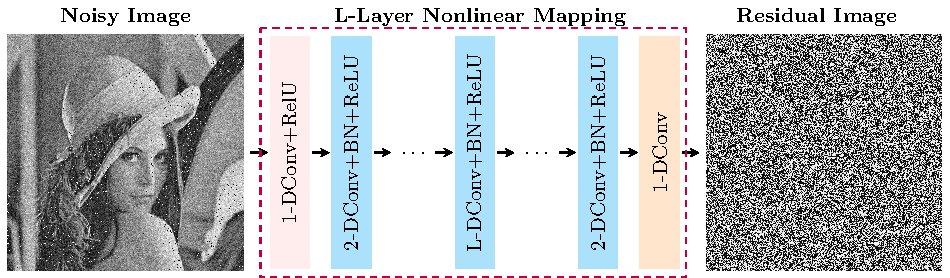
\includegraphics[width=\linewidth]{2-8}
	\caption{IRCNN网络架构示意图}\label{fig:2-8}
\end{figure}

\section{本章小结}
本章首先概述了非凸优化理论的基本问题与基本算法,其次介绍了深度学习领域的深度卷积神经网络结构与基于深度学习的图像去噪算法,最后给出了图像去噪领域中两种典型深度卷积神经网络去噪器DnCNN和IRCNN的网络架构。



  % !Mode:: "TeX:UTF-8"
\chapter{基于共识方程的编码衍射成像算法}
\label{chap:ce}
\section{引言}
病态反问题在计算机视觉任务的建模中随处可见,编码衍射成像系统中的相位恢复作为典型的病态反问题,其求解往往由于模型高度非凸等原因异常困难。最近,随着机器学习中非凸优化理论的蓬勃发展,基于即插即用先验的近邻算法在解决病态反问题中崭露头角。这类方法将基于残差学习的图像去噪算子和数值优化方法相结合,利用学习的深度卷积神经网络代替模型中求解困难或复杂的部分,在底层计算机视觉问题上取得了巨大成功。然而,将学习的深度卷积神经网络嵌入到迭代算法中并非易事,大部分方法都是通过特定问题的优化算法结构进行指导来达到最佳的图像重建效果,而非像数值优化方法那样通过严格的理论分析来保障求解的稳定性与可靠性。因此,对非凸问题而言目前的即插即用算法是否收敛最优解仍无法保证。

为了解决该疑惑,本章试图深入分析可学习迭代方法优越性能表象下的本质,即通过理论分析解释这类方法能够取得成功的根本原因。基于该目标,本章首先利用即插即用ADMM和FBS(Forward-backward Splitting)算法求解编码衍射模型中的相位恢复问题,其次分析了基于RED先验的prDeep算法,最后从共识优化到公式方程,提出了基于Two-agent共识方程的编码衍射相位恢复算法框架,如图\ref{fig:3-1}所示,并给出收敛性分析来表明TACE迭代算法在给定算子非扩张的假设下可以收敛到共识方程的一个不动点。因为TACE的算法中数据保真项的近邻算子与去噪算子相互独立,故该算法可用多线程并行实现。考虑到目前基于深度学习的去噪器与数据保真项的近邻算子在GPU上运行速度相当,而传统的BM3D等算法运行在CPU上,如果将BM3D去噪算子加入共识方程,势必会导致该算法运行时间延长,所以暂不考虑Multi-agent共识方程问题。
\begin{figure}[!hptb]
	\centering
	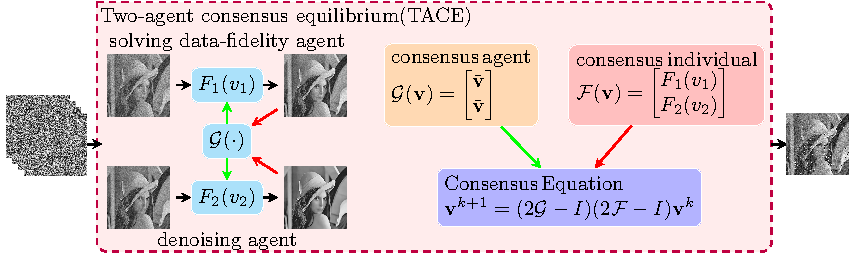
\includegraphics[width=\linewidth]{3-1}
	\caption{TACE算法示意图}\label{fig:3-1}
\end{figure}

\section{图像去噪算法的利普希茨约束}
当前流行的即插即用算法一般为非凸框架,虽然在图像反问题的求解上表现出色,但是算法的收敛性无法保证。为解决上述问题,Liu等人提出了实谱归一化(Real Spectral Normalization,realSN)方法以约束去噪器残差映射的利普希茨常数等于$1$,并给出了即插即用算法的收敛性保证\supercite{Ernest}。压缩映射与非扩张算子的定义如下所示:
\begin{definition} \label{def:3-1}
	算子$T:\mathbb{R}^n\to\mathbb{R}^n$是$L$-Lipschitz连续的,如果它满足
	\begin{equation}
		\Vert{T(x)-T(y)}\Vert_2^2\leq{L}\Vert{x-y}\Vert_2^2,\quad{\forall{x,y\in\mathbb{R}^n}}.
	\end{equation}
	若$L=1$,则$T$为非扩张算子;若$L<1$,则$T$为收缩算子。
\end{definition}

从泛函拟合的角度出发,DnCNN和IRCNN可用$D(y)=y-R(y)$表示,此时残差映射为$R(y)=y-D(y)=(I-D)(y)$。约束去噪器残差映射的利普希茨常数等价于迫使其满足如下假设:
\begin{assumption} \label{assumption:3-1}
	$\exists{\epsilon\ge{0}}$,$D_{\sigma}(x)\colon\mathbb{R}^n\to\mathbb{R}^n$对于$\forall{x,y}\in\mathbb{R}^n$满足:
	\begin{equation} 
		\Vert{(D_\sigma-I)(x)-(D_\sigma-I)(y)}\Vert^2\leq{\epsilon^2\Vert{x-y}\Vert^2}.
	\end{equation}	
\end{assumption}
%\begin{definition} \label{define:spectral-radius}
%	谱半径:$A_{n\times{n}}$的特征值为$\lambda_i$,$1\leq{i}\leq{n}$,那么其谱半径定义为
%	\begin{equation}
%		\rho(A) = \max_{1\leq{i}\leq{n}}\vert{\lambda_i}\vert.
%	\end{equation}
%\end{definition}
%\begin{definition} \label{define:spectral-norm}
%	谱范数:$A_{n\times{n}}$的谱范数定义为
%	\begin{equation}
%		\Vert{A}\Vert=\sup_{\Vert{x}\Vert=1}{\Vert{Ax}\Vert_2}.
%	\end{equation}
%\end{definition}
%bthm
%\begin{theorem} \label{third:com-spectral}
%	对于任意方阵$A_{n\times{n}}$,有
%	\begin{equation}
%		\Vert{A}\Vert=(\rho(A^{\mathit{H}}A))^{\frac{1}{2}}.
%	\end{equation}
%\end{theorem}
%\begin{lemma} \label{}
%	对于任意方阵$A_{n\times{n}}$,有
%	\begin{equation}
%		\Vert{A}\Vert\geq{\rho(A)}.
%	\end{equation}
%\end{lemma}
因DnCNN与IRCNN去噪器由卷积层、BN层、ReLU层复合而成,如图\ref{fig:2-7}和图\ref{fig:2-8}所示。此外ReLU函数的导数为1,故只需对卷积核$\mathcal{K}:\mathbb{R}^{C_{in}\times{h}\times{w}}\to{\mathbb{R}^{C_{out}\times{h}\times{w}}}$执行实谱归一化,其主要步骤如下所示:

(1)对卷积核应用一次幂迭代计算奇异值对应的特征向量:
\begin{equation} \label{equation:3-1}
	\begin{cases}
		V_{l}\leftarrow{\mathcal{K^\mathit{H}}(U_l)/\Vert{\mathcal{K^\mathit{H}}(U_l)}\Vert_2},\\
		U_{l}\leftarrow{\mathcal{K}(V_l)/\Vert{\mathcal{K}(V_l)}\Vert_2}.\\
	\end{cases}
\end{equation}

(2)计算卷积核的谱范数并进行归一化操作:
\begin{equation} \label{equation:3-2}
	\mathcal{K}_l\leftarrow{\mathcal{K}_l/\rho{(\mathcal{K_l})}}.
\end{equation}
其中$U_l\in\mathbb{R}^{C_{out}\times{h}\times{w}}$,$V_l\in\mathbb{R}^{C_{in}\times{h}\times{w}}$,$\rho(\mathcal{K}_l)=\left<{U_l, \mathcal{K}_l(V_l)}\right>$。以$\rho(\mathcal{K_l})/c_l$替代$\rho(\mathcal{K_l})$,此时深度学习去噪器利普希茨常数的上界为$C=\prod_{l=1}^L{c_l}$。关于去噪器有如下引理:
\begin{lemma} \label{lemma:3-1}
	若$D_{\sigma}:\mathbb{R}^n\to\mathbb{R}^n$满足假设\ref{assumption:3-1},当且仅当
	\begin{equation}
		\frac{1}{1+\epsilon}D_{\sigma}.
	\end{equation}
	为$\frac{\epsilon}{1+\epsilon}$-平均算子。更为一般地,$\frac{1}{1+2\epsilon}(2D_{\sigma}-I)$为$\frac{2\epsilon}{1+2\epsilon}$-平均算子。
\end{lemma}
当假设\ref{assumption:3-1}中的$\epsilon=1$时,由引理\ref{lemma:3-1}推的$\frac{1}{2}D_{\sigma}$为$\frac{1}{2}$-平均算子,亦为固定非扩张算子。

\section{基于即插即用先验的编码衍射成像算法}
对偶分解或ADMM等分解方法可以解决与图相关的问题,例如最大后验概率估计(Maximum Posteriori Estimation,MAP)推理和图匹配。其主要思想是将原始复杂图分解为更简单的子图,然后使用不同的机制重新组合这些子图。。大量图像重建任务可以表示为MAP问题\supercite{ZhangKai,Shunsuke,Stanley},其基本框架如下所示:
\begin{equation} \label{problem:3-1}
	\begin{aligned} 
		\hat{x}&=\arg\max_{x}\ p(x\;\vert\;y) \\
			   &=\arg\max_{x}\ -\log{p(y\;\vert\;x)-\log{p(x)}}.
	\end{aligned}
\end{equation}
其中条件概率${p(y\;\vert\;x)}$表示图像反问题的前向模型,$p(x)$表示待恢复图像的先验分布。MAP为基于模型的图像重建方法,其关键在于寻找待恢复图像的有效先验知识。根据帕累托法则,待恢复图像的先验知识起关键性作用。另外,MAP等价于求解如下优化问题:
\begin{equation} \label{problem:3-2}
	\mathop{\text{minimize}}\limits_{x}\quad f(x)+\lambda{g(x)}.
\end{equation}
其中$f(x)\overset{\underset{\mathrm{def}}{}}{=}{-\log{p(y\vert{x})}}$为${p(y\;\vert\;x)}$的负最大似然估计函数,$g(x)\overset{\underset{\mathrm{def}}{}}{=}{-\log{p(x)}}$。问题\eqref{problem:3-2}为标准的无约束优化问题。站在贝叶斯优化的视角,编码衍射成像模型的数据保真项应正比于其条件概率对应的负最大似然函数。一般地,编码衍射成像的观测模型为$y=\vert{Ax}\vert+w$,其中$w\sim{C\mathcal{N}(0,\sigma_w{I})}$,则负的最大似然函数$-\log{p(y\vert{x})}\propto\frac{1}{2}{\Vert{y-\vert{Ax}\vert}\Vert_2^2}$。此时求解编码衍射中的PR问题,只需令$f(x)=\frac{1}{2}{\Vert{y-\vert{Ax}\vert}\Vert_2^2}$即可。另外,图像的先验知识$\log{p(x)}$对非线性图像反问题求解至关重要。人们根据图像的先验分布提出了大量有效的图像去噪算法:基于稀疏表示的K-SVD去噪方法利用图像块的自适应字典学习有效地去除噪声;BM3D综合稀疏性和局部自相似性取得了传统算法中SOTA的结果。

相反地,深度学习技术利用大量数据学习图像先验,基于监督学习的DnCNN和IRCNN从海量的训练数据中学习到的先验知识具有更强的泛化能力和更复杂的参数化表达,且无需调节算法参数以适应不同的应用场景\supercite{Kai,ZhangKai};基于无监督学习的深度图像先验方法利用生成器网络的结构足以在任何学习之前捕获大量的低级图像统计信息进行去噪处理;传统的去噪算法的深度展开(Deep Unrolling)策略也在图像去噪领域取得了一定的进展\supercite{Yan,Chenyang,Hasselt,Schaul,Bellemare,Matteo,Dabney1,Dabney2,Volodymyr}。一般地,图像先验$\log{p(x)}$有明确的数学表达式,这表明优化问题\ref{problem:3-2}是显式地,仍属于优化领域的范畴。但是当图像先验$\log{p(x)}$不能转化为数学表达式,优化问题\eqref{problem:3-2}为隐式地,脱离了优化领域的范畴。如何利用去噪器构造图像或隐式地嵌入到结构化求解算法中需要进一步研究。即插即用ADMM算法是一种强大的图像重建框架,允许高级图像去噪先验集成到物理系统前向模型中生成高质量的图像重构结果。Venkatakrishnan等人首次提出即插即用先验的概念,根据ADMM框架的特殊结构,提出了即插即用先验(Plug-and-Play Priors, $P^3$)算法\supercite{Stanley}。该算法在求解正则化的图像反问题时,将ADMM框架分成数据保真项模型和去噪模型(先验模型),数据保真项模型通过简单的梯度下降法或存在快速求解算法(去模糊中的模糊核为循环矩阵,可用快速傅里叶变换求解),去噪模型利用传统的去噪算法或基于深度学习的去噪算子进行求解。 

由于去噪模型可利用不同的去噪算子进行求解,$P^3$算法能够利用不同的图像先验进行图像重建。Chan等人假设去噪器有界:$\Vert{D_{\sigma}(x)-x}\Vert/n\leq{\sigma^2C}$,而有界去噪器是渐近不变地:$D_{\sigma}\to{0}(\sigma\to{0})$。之后,Chan等人从理论上在$f(x)$的$\mu$-强凸的假设下,证明了即插即用ADMM算法的不动点收敛性\supercite{ZhangKai}。Metzler等人将BM3D去噪算子引入到近似消息传递算法的迭代中,隐式地利用即插即用先验求解压缩相位恢复问题,并且在去噪器满足假设:$\mathbb{E}\left[\Vert{D_{\sigma}(x+\sigma\epsilon)-x}\Vert^2/n\right]\leq{\kappa\sigma^2}$和观测矩阵$\{a_j\overset{\underset{\mathrm{iid}}{}}{\sim}\mathcal{N}(0,I_n)\}_{1\leq {j\leq{m}}}$下,证明了prGAMP算法的收敛性\supercite{Metzler4}。数值实验结果表明prGAMP算法能够从欠采样测量数据中重建高质量图像。

基于隐式先验的图像重建算法具有有效、灵活的特点,该类算法能够利用高级去噪器将图像的先验知识隐式地引入到图像重建中。但是即插即用ADMM算法严重依赖于ADMM算法的结构,并且为非凸框架,收敛性与收敛速度无法保证。为了有效解决该问题,Liu等人提出实谱归一化技术对深度去噪器DnCNN进行利普希茨约束\supercite{Ernest}。令人诟病的是该方法仅限于深度学习去噪器,并未涉及图像反问题中的数据保真项,使得基于即插即用先验的ADMM算法应用范围有限。

鉴于此,Romano等人提出了显式的RED先验,与隐式即插即用先验的不同之处在于其具有明确的数学表达式,因而优化问题\eqref{problem:3-2}明确。此外,Siavash等人构造了另一种显式的自编码先验$\frac{1}{2}\Vert{x-D_{\sigma}(x)}\Vert_2^2$\supercite{Siavash,Yankun,Zhang}。另外,基于即插即用先验的的PR算法能够依据最大似然估计设计针对不同测量系统噪声类型的数据保真项,但Metzler发现泊松噪声可以应用数据保真项$\frac{1}{2}{\Vert{y-\vert{Ax}\vert}\Vert_2^2}$进行求解,打破了依据最大似然估计设计数据保真项的限制。以下介绍两种基于近邻算子的即插即用算法。

\subsection{即插即用ADMM算法}
即插即用算法是将ADMM或其他邻近算法与高级去噪器先验相结合的非凸框架。PR问题中代价函数$f(x)=\frac{1}{2}{\Vert{y-\vert{Ax}\vert}\Vert_2^2}$非凸、非光滑。利用ADMM方法求解优化问题\eqref{problem:3-2},该问题等价于
\begin{equation} \label{problem:3-3}
	\begin{aligned} 
		&\text{minimize}\quad\frac{1}{2}{\Vert{y-\vert{Az}\vert}\Vert_2^2}+\lambda{g(x)} \\
		&\text{subject\ to}\quad x-z=0 \\
	\end{aligned}
\end{equation}
上述优化问题转化为以下增广拉格朗日函数为:
\begin{equation} \label{equation:3-3}
	\begin{aligned}
		L_{\rho}(x,y,z)&=\frac{1}{2}{\Vert{y-\vert{Az}\vert}\Vert_2^2}+\lambda{g(x)}+y^\top(x-z)+\frac{\rho}{2}\Vert{x-z}\Vert_2^2\\
		&=\frac{1}{2}{\Vert{y-\vert{Az}\vert}\Vert_2^2}+\lambda{g(x)}+\frac{\rho}{2}\Vert{x-z+u}\Vert_2^2.
	\end{aligned}
\end{equation}
其中$u=\frac{y}{\rho}$表示尺度对偶变量,ADMM方法通过求解以下子问题(对于第$k+1$次迭代)对上述优化问题进行求解:

(1)图像$x$去噪子问题:固定$z,u$,问题\eqref{equation:3-3}相当于求解以下子问题:
\begin{equation} \label{}
	x^{k+1}=\arg\min_{x}=\lambda{g(x)}+\frac{\rho}{2}\Vert{x-z^k+u^k}\Vert_2^2.
\end{equation}
上述子问题与基于先验的去噪问题相似,故数值解为:
\begin{equation} \label{third:x-step}
	x^{k+1}:=D_{\sigma}(z^k-u^k).
\end{equation}

(2)辅助变量$z$更新子问题:固定$x,u$,问题\eqref{equation:3-3}相当于求解以下子问题:
\begin{equation} \label{equation:3-4}
	z^{k+1}=\arg\min_{z}=\frac{1}{2}{\Vert{y-\vert{Az}\vert}\Vert_2^2}+\frac{\rho}{2}\Vert{x^{k+1}-z+u^k}\Vert_2^2.
\end{equation}
应用不动点迭代,上述问题的数值解为:
\begin{equation} \label{equation:3-5}
	z^{k+1}:=\frac{1}{1+\rho}\left({A^{\mathit{H}}\left(\frac{Az^k}{\vert{Az^k}\vert}\odot{y}\right)}+\rho{(x^{k+1}+u^k)}\right).
\end{equation}

(3)对偶变量$u$更新:
\begin{equation} \label{equation:3-6}
	u^{k+1}:=u^k+x^{k+1}-z^{k+1}.
\end{equation}

(4)最后应用内插技术得到:
\begin{equation} \label{equation:3-7}
	\hat{x}^{k+1} := (1-\alpha)\hat{x}^k+\alpha{x^k}.
\end{equation}
算法的终止条件利用优化变量的相对残差范数(relative residual, res)进行度量,其定义为:
\begin{equation} \label{equation:3-8}
	\text{res}=\frac{\Vert{x^{k+1}-x^k}\Vert_2}{\max\{1, \Vert{x^k}\Vert_2\}}.
\end{equation}
当$\text{res}\leq{\epsilon}$($\epsilon$为相对误差限)或达到最大迭代次数算法终止迭代。算法\ref{algorithm:3-1}总结了即插即用ADMM算法。
\begin{algorithm}[!htbp]
	\setstretch{1.4}\zihao{-4}
	\caption{即插即用ADMM(PnP-ADMM)}
	\label{algorithm:3-1}
	\begin{algorithmic}[1]
		\REQUIRE	观测值$y\in \mathbb{R}^m$; % this command shows "Input"
		\ENSURE		% this command shows "Initialized"
		$\rho > 0, \alpha\in (0,1), \sigma\in[1,50], (x^0,z^0,u^0)$随机; \\
		\WHILE {\emph{not converged}}
		\STATE	$x^{k+1}:=(1-\alpha)x^k + \alpha{D_{\sigma}(z^k-u^k)}$; \\ % line number at left side
		\STATE	$z^{k+1}:=\frac{1}{1+\rho}\left({A^{\mathit{H}}\left(\frac{Az^k}{\vert{Az^k}\vert}\odot{y}\right)}+\rho{(x^{k+1}+u^k)}\right)$; \\	% line number at left side
		\STATE	$u^{k+1}:=u^k+x^{k+1}-z^{k+1}$; \\ % line number at left side
		\ENDWHILE
		\RETURN 重构图像$x^{k+1}$. % this command shows "Output"
	\end{algorithmic}
\end{algorithm}

\subsection{即插即用邻近梯度算法}
利用邻近梯度方法求解优化问题\eqref{problem:3-2},第$k+1$次迭代的公式如下所示:
\begin{equation} \label{equation:3-9}
	x^{k+1}:=D_{\sigma}\left(x^k-\eta_k{A^{\mathit{H}}\left({Ax^k-y\odot{\frac{Ax^k}{\vert{Ax^k}\vert}}}\right)}\right).
\end{equation}
加速近邻梯度法在外推处求代价函数的梯度,可看作是Nerterov's加速算法的推广。其对应的第$k+1$次迭代的公式如下所示:
\begin{equation} \label{equation:3-10}
	\begin{cases}
		v^{k+1}:=x^k+\omega_k(x^k-x^{k-1}), \\
		x^{k+1} := D_{\sigma}\left(v^k-\eta_k{A^{\mathit{H}}\left({Av^k-y\odot{\frac{Av^k}{\vert{Av^k}\vert}}}\right)}\right). \\
	\end{cases}
\end{equation}
其中$\eta_k\in(0,\frac{1}{L})$,$L$为数据保真项梯度的利普希茨常数,而数据保真项非光滑,故数据保真项的梯度不满足利普希茨连续性条件。$\omega_k$的典型值为$\frac{k}{k+3}$。上述算法的迭代终止条件与算法\ref{algorithm:3-1}相同。算法\ref{algorithm:3-2}总结了即插即用邻近梯度算法。
\begin{algorithm}[!htbp]
	\setstretch{1.4}\zihao{-4}
	\caption{即插即用FBS(PnP-FBS)}
	\label{algorithm:3-2}
	\begin{algorithmic}[1]
		\REQUIRE	观测值$y\in \mathbb{R}^m$;	% this command shows "Input"
		\ENSURE		% this command shows "Initialized"
		$\eta_k\in(0,\frac{1}{L}),\sigma\in[1,50],x^0$随机; \\
		\WHILE {\emph{not converged}}
		\STATE $x^{k+1}:=D_{\sigma}\left(x^k-\eta_k{A^{\mathit{H}}\left({Ax^k-y\odot{\frac{Ax^k}{\vert{Ax^k}\vert}}}\right)}\right)$;\\ % line number at left side
		\ENDWHILE
		\RETURN 重构图像$x^{k+1}$. % this command shows "Output"
	\end{algorithmic}
\end{algorithm}

\section{基于去噪正则化先验的编码衍射成像算法}
RED(Regularization by Denoising)最早由Romano等人提出\supercite{Romano,Hong,Zihui},用于解决图像去模糊、单幅图像超分辨率、相位恢复等图像反问题。RED正则项的数学表达式为:
\begin{equation} \label{equation:3-11}
	g(x)=\frac{1}{2}x^\top(x-D_{\sigma}(x)).
\end{equation}
若式\eqref{equation:3-11}满足:

(1)局部齐次性(local homogeneity):$D_{\sigma}(Cx)=CD_{\sigma}(x),\vert{C-1}\vert\leq\epsilon$;

(2)其梯度谱半径小于等于$1$:$\rho(\nabla_{x}D_{\sigma}(x))\leq{1}$;

由(1)(2)可推的$g(x)$为凸函数,并且$\nabla{g(x)}=x-D_{\sigma}(x)$。因为$\rho(\nabla_{x}D_{\sigma})\leq\Vert{D_{\sigma}}\Vert_2$,所以实谱归一化的DnCNN和IRCNN满足条件(2)。图\ref{fig:3-1}为$D_{\sigma}((1+\epsilon)x)$相对于$(1+\epsilon)D_{\sigma}(x)$的散点图,括号中的数字表示两者的方差,实验图像$x$为Lenna,$\sigma=15$。可见DnCNN、IRCNN、Realsn-DnCNN和Realsn-IRCNN均满足条件(1)。
\begin{figure}[!htbp]
	\vspace*{-0.05\linewidth}
	\centering
	\subfigure[DnCNN(3.74e-4)]{
		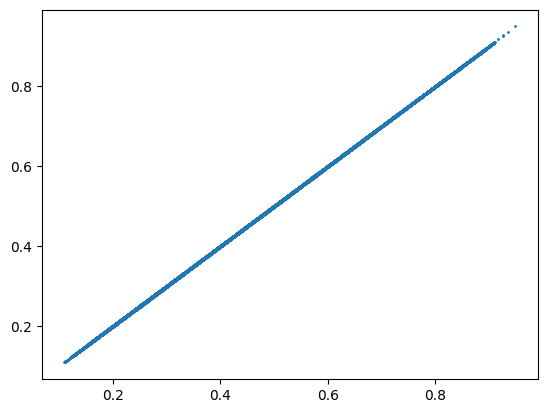
\includegraphics[width=0.4\linewidth]{3-2-1}  
	}
	\subfigure[IRCNN(3.33e-4)]{
		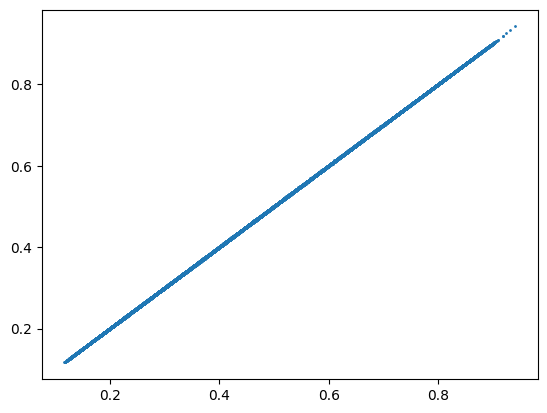
\includegraphics[width=0.4\linewidth]{3-2-2}  
	}
	
	\subfigure[realSN-DnCNN(3.49e-4)]{
		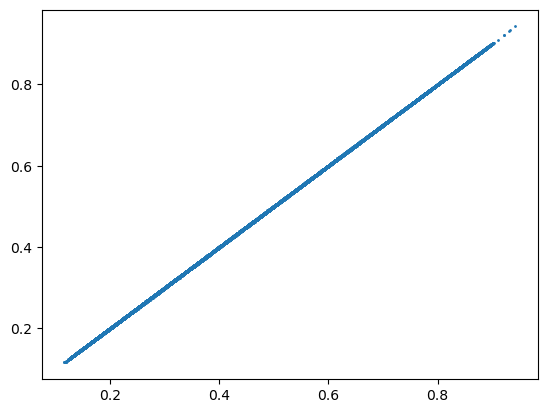
\includegraphics[width=0.4\linewidth]{3-2-3}  
	}
	\subfigure[realSN-IRCNN(3.47e-4)]{
		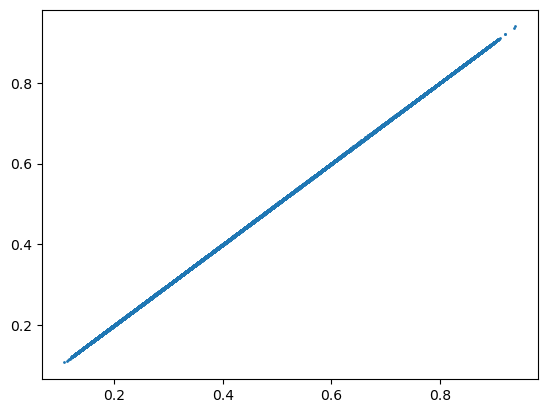
\includegraphics[width=0.4\linewidth]{3-2-4}  
	}
	\caption{去噪器DnCNN与IRCNN的局部齐次性评估散点图} \label{fig:3-2}
\end{figure}

RED正则项可看作是图像$x$与相应残差$x-D_{\sigma}(x)$的非归一化自相关性,当残差趋于零值时,图像$x$应满足$x\approx{D_{\sigma}(x)}$;当图像$x$与其残差图像$x-D_{\sigma}(x)$不相关时,$g(x)$趋向于零值。Metzler等人将RED作为相位恢复的正则项,提出了基于RED先验的prDeep算法\supercite{Metzler1}。prDeep算法用于恢复含泊松噪声的观测值,但其对应的PR问题如下所示:
\begin{equation} \label{problem:3-4}
	\mathop{\text{minimize}}\limits_{x}\quad \frac{1}{2}{\Vert{y-\vert{Ax}\vert}\Vert_2^2} + \frac{\lambda}{2}x^\top(x-D_{\sigma}(x)).
\end{equation}
RED先验对应的proximal算子为:
\begin{equation} \label{equation:3-12}
	\begin{aligned} 
		\text{prox}_{g}(v)&=\arg\min_{x}\frac{\lambda}{2}x^\top(x-D_{\sigma}(x))+\frac{1}{2}\Vert{x-v}\Vert_2^2,\\
		&=u_{\infty},
	\end{aligned}
\end{equation}
其中$u_j=\frac{1}{1+\lambda}(u_{j-1}+\lambda{D_{\sigma}(u_{j-1})})$,$u_0=v$。由于去噪器迭代存在大量计算,故一般取$j=1$。Metzler利用FASTA算法进行求解,与PnP-FBS算法基本相同,但FASTA采取自适应学习率和反向线性搜索技术进行加速,使得重建速度优于PnP-FBS\supercite{Goldstein}。有趣的是,PrDeep作者在实验中选取噪声强度固定的去噪算子,但本章发现选取$\sigma\in[1,50]$的盲去噪器仍可以取得与之相当的重构效果。

\section{从共识优化到共识方程}
图像重构中正则化反问题的方法由于其能够结合复杂的物理传感器模型和有效的正则化特点而得到广泛应用\supercite{Gregery,Joon,Kamilov,Siavash,Yankun,Zhang}。基于即插即用先验的方法提供了一个使用高级去噪算法作为正则化器的框架。然而,将正则化的反问题作为优化问题的解决方案,限制了可能的正则化条件和物理传感器模型的多样性。

在一般的动力系统中,存在多个传感器收集多组数据的情况。其对应的代价函数被分解为多个辅助函数之和的形式:
\begin{equation} \label{problem:3-5}
	\mathop{\text{minimize}}\limits_{x}\quad f(x)=\sum_{i=1}^{N}\mu_{i}f_i(x),
\end{equation} 
其中$x\in\mathbb{R}^n$,$f_i\colon\mathbb{R}^n\to\mathbb{R}\cup\{+\infty\}$,权重$\mu_{i}>0$,$i=1,\ldots,N$并且$\sum_{i=1}^{N}{u_i}=1$。在共识优化中,最小化原始代价函数可重新表述为辅助函数之和的最小化,约束中每个分离的优化变量$x_i$共享同一个$x$:
\begin{equation} \label{problem:3-6}
	\begin{aligned}
		&\text{minimize}\quad\sum_{i=1}^{N}\mu_{i}f_i(x) \\
		&\text{subject\ to}\quad{x_{i} = x,\ i=1,\ldots,N} \\
	\end{aligned}
\end{equation}
其中$x\in\mathbb{R}^n$,$x_{i}\in\mathbb{R}^n$。上述优化问题可用ADMM算法进行求解。正则化的反问题和优化问题得益于广泛的理论和强大的算法,但是,大量有效、简单的去噪算法不能嵌入到优化算法中。即使优化算法(例如ADMM)的结构性允许嵌入,但该算法一般为隐式模型,无法保证去噪迭代对应近邻算子的存在,导致代价函数无法显示地确定。再者,该算法为非凸算法,收敛性无法保证。不过该算法一般收敛到不动点,它对去噪迭代通过迭代控制前向模型的近邻算子中的步长和去噪器的噪声强度鲁棒。以下将从共识优化推到共识方程:

假设$f_i\colon\mathbb{R}^n\to\mathbb{R}\cup\{+\infty\}$为闭凸函数,$F_i$为相应的近邻算子,其由式\eqref{proximal-operator}定义。优化问题\eqref{problem:3-6}对应的拉格朗日函数为
\begin{equation} \label{equation:3-13}
	L(x,(x_i)_{i=1}^N,(\lambda_i)_{i=1}^N)=\sum_{i=1}^{N}(\gamma\mu_{i}f_i(x_i)+\lambda_i^\top(x-x_i)).
\end{equation}
其中$\gamma$为近邻算子$F_i$的尺度因子,$\lambda_i$为朗格朗日乘子向量。如果$f_i$是凸函数和下半连续的,则KKT条件是最优解的充分条件。最优解$(x^*,(x_i^*)_{i=1}^N,(\lambda_i^*)_{i=1}^N)$由式\eqref{equation:3-14}给出:
\begin{equation} \label{equation:3-14}
	\begin{aligned}
 		\nabla_x{L(x^*,(x_i^*)_{i=1}^N,(\lambda_i^*)_{i=1}^N)}&=0, \\
		\partial_{x_i}{L(x^*,(x_i^*)_{i=1}^N,(\lambda_i^*)_{i=1}^N)}&\ni{0},\quad\forall{i=1,\ldots,N}, \\
		x_i^*-x^*&=0,\quad\forall{i=1,\ldots,N}. \\
	\end{aligned}
\end{equation}
其中$\partial_{x_i}$表示子微分。式\eqref{equation:3-14}转化为:
\begin{equation} \label{equation:3-15}
	\begin{aligned}
		\sum_{i=1}^{N}\lambda_i&=0, \\
		\gamma\mu_i\partial{f_i(x_i^*)}&\ni{\lambda_i^*},\quad\forall{i=1,\ldots,N}, \\
		x_i^*&=x^*,\quad\forall{i=1,\ldots,N}. \\
	\end{aligned}
\end{equation}
定义$u_i^*=\lambda_i^*/\mu_i$,将$x_i^*=x^*$代入$\gamma\mu_i\partial{f_i(x_i^*)}\ni{\lambda_i^*}$得到$\gamma\partial{f_i(x^*)}\ni{u_i^*}$。再两边同时加$x^*$得到$x^*+\gamma\partial{f_i(x^*)}\ni{x^*+u_i^*}$。此式等价于
\begin{equation} \label{equation:3-16}
	(I+\gamma\partial{f_i})(x^*)\ni{x^*+u_i^*}.
\end{equation}
由式\eqref{equation:3-16}推的$x^*=(I+\gamma\partial{f_i})^{-1}(x^*+u_i^*)$,此式正是$f_i$的近邻算子$F_i$。由以上可得共识方程为
\begin{equation} \label{equation:ce}
	\begin{aligned}
		F_i(x^*+u_i^*)&=x^*,\quad{i=1,\ldots,N,} \\
		\overline{\mathbf{u}}_\mu^*&=0. \\
	\end{aligned}
\end{equation}
其中$\mathbf{u}\in\mathbb{R}^{nN}$为$u_1,\ldots,u_N$的列向堆叠,$\overline{\mathbf{u}}_\mu$为权重平均$\sum_{i=1}^{N}\mu_i{u_i}$。

\section{基于共识方程的编码衍射成像算法}
共识均衡(Consensus Equilibrium)旨在利用迭代求解算法使得不同算子达到平衡点,类似于博弈论中的纳什均衡(Nash Equilibrium)。共识方程\eqref{equation:ce}脱离了优化算法的范畴,求解目标有着清晰的数学表示,是一个优雅的数学框架。共识方程可将基于优化的算子(近邻算子)或基于非优化的算子(去噪器)嵌入其中,每一个算子代表一个博弈主体,允许多个主体参与非合作式博弈。

Chan等人将CE用于图像盲去噪与非理想背景中前景自动提取\cite{Gregery,Xiran},在噪声未知的情况下取得了SOTA结果\supercite{Gregery,Joon,Xiran}。但对于确定的噪声强度的噪声,去噪性能不如单个DnCNN。基于多代理CE的前景自动提取算法融合TV去噪、背景提取、 Alpha matting等代理,以处理背景不完美的复杂场景。受到Chan等人工作的启发,本节将CE用于编码衍射模型中的相位恢复问题,提出了TACE(Two-agent Consensus Equilibrium)算法,以下为主要求解步骤。

CE方程为无约束的方程组,可用非扩张算子的不动点理论去分析其收敛性。另外,非扩张算子的预处理各向异Mann迭代可用于算法的加速处理。首先,定义如下概念:
\begin{equation} \label{equation:agent}
	\mathbf{F}(\mathbf{v})
	=
	\begin{pmatrix}
		F_1(v_1) \\ F_2(v_2)
	\end{pmatrix} 
	=	
	\begin{pmatrix}
		((1-\theta)I+\theta\text{prox}_{\gamma{f}})(v_1) \\ \frac{1}{2}D_{\sigma}(v_2)
	\end{pmatrix} 
	\quad and \quad
	\mathbf{G}_{\mu}(\mathbf{v})
	=
	\begin{pmatrix}
		\overline{\mathbf{v}}_{\mu} \\ \overline{\mathbf{v}}_{\mu} 
	\end{pmatrix} 
\end{equation}
其中
\begin{equation} \label{equation:3-17}
	\begin{aligned}
		\text{prox}_\gamma{f}(v_1)&=\arg\min_{x}
		\frac{1}{2}{\Vert{y-\vert{Ax}\vert}\Vert_2^2} +\frac{1}{2\gamma}{\Vert{x-v_1}\Vert_2^2}, \\
		&\approx\frac{1}{1+\gamma}\left({\gamma A^{\mathit{H}}\left(\frac{Ax^k}{\vert{Ax^k}\vert}\odot{y}\right)}+v_1^k\right),\; k\geq{0}.
	\end{aligned}
\end{equation}
如果$\mathbf{v}^*=\hat{x}^*+\mathbf{u}^*$,其中$\hat{x}=(x,x)^\top$,满足$\overline{\mathbf{v}}_{\mu}^*=x^*$,并且
\begin{equation} \label{equation:3-18}
	\left({2\mathbf{G}_{\mu}-I}\right)\left({2\mathbf{F}-I}\right)\mathbf{v}^*=\mathbf{v}^*.  
\end{equation}
则$(x^*,\mathbf{u}^*)$为CE方程\ref{equation:ce}当$N=2$时的最优解。定义$\mathbf{T}\overset{\underset{\mathrm{def}}{}}{=}\left({2\mathbf{G}_{\mu}-I}\right)\left({2\mathbf{F}-I}\right)$,应用非扩张算子的Mann迭代可得CE方程的第$k$次迭代为:
\begin{equation} \label{equation:3-19}
	\begin{aligned}
		\mathbf{v}^{k+1}&:=(1-\beta)\mathbf{v}^{k}+\beta\mathbf{T}(\mathbf{v}^{k}),	\\
		x^{k+1}&:=\overline{\mathbf{v}}^{k+1}.
	\end{aligned}
\end{equation}
最后再对优化变量$x$应用内插技术得到以下算法:
\begin{equation} \label{equation:3-20}
	\begin{aligned}
		\mathbf{v}^{k+1}&:=(1-\beta)\mathbf{v}^{k}+\beta\mathbf{T}(\mathbf{v}^{k}),	\\
		x^{k+1}&:=(1-\alpha)x^k + \alpha\overline{\mathbf{v}}^{k+1}.
	\end{aligned}
\end{equation}
算法\ref{algorithm:3-3}总结TACE算法的实现细节。
\begin{algorithm}[!htbp]
	\setstretch{1.4}\zihao{-4}
	\caption{TACE}
	\label{algorithm:3-3}
	\begin{algorithmic}[1]
		\REQUIRE	观测值$y\in \mathbb{R}^m$; % this command shows "Input"
		\ENSURE		% this command shows "Initialized"
		$\alpha,\beta\in (0,1), \theta\in(0,\frac{1}{2}],\gamma{=1}, sigma\in[1,50], \mu_{1}=\mu_{2}=\frac{1}{2},(\mathbf{v}^0,x^0)$随机; \\
		\WHILE {\emph{not converged}}
		\STATE	$\mathbf{v}^{k+1}:=(1-\beta)\mathbf{v}^{k}+\beta\mathbf{T}(\mathbf{v}^{k})$; \\  % line number at left side
		\STATE	$x^{k+1}:=(1-\alpha)x^k + \alpha\overline{\mathbf{v}}_{\mu}^{k+1}$; \\	% line number at left side
		\ENDWHILE
		\RETURN 重构图像$x^{k+1}$.  % this command shows "Output"
	\end{algorithmic}
\end{algorithm}
需要指出的是,当$N=2$时,PnP-ADMM和TACE的最优解等价,均收敛到不动点$(x^*, u^*)$,即满足式\eqref{equation:3-21}:
\begin{equation} \label{equation:3-21}
	\begin{aligned}
		\text{prox}_{\gamma{f}}(x^*-u^*)&=x^*, \\
		D_{\sigma}(x^*+u^*)&=x^*. \\
	\end{aligned}
\end{equation}
不失一般性,TACE算法的推广版本MACE(Multi-Agent Consensus
Equilibrium)算法的第$k+1$次迭代如图\ref{fig:3-3}所示。图\ref{fig:3-3}中$F_{1},\ldots,F_{N}$表示$N$个代理。
\begin{figure}[!hptb]
	\centering
	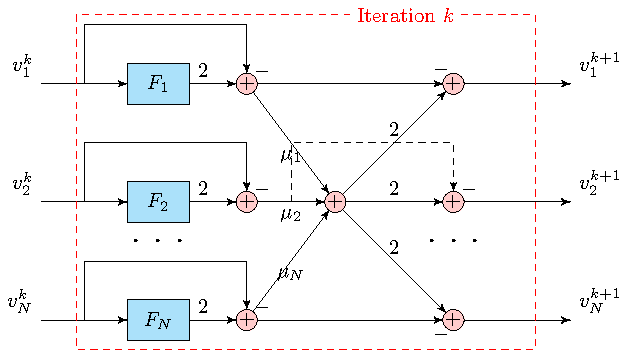
\includegraphics[width=0.8\linewidth]{3-3}
	\caption{MACE算法第$k+1$次迭代示意图}\label{fig:3-3}
\end{figure}

最后,在理论层面当$F^\prime{s}$满足假设\ref{assumption:3-2}时,本章通过严格的数学证明给出了MACE算法的收敛性,此时文献\cite{Xiran}的假设条件可看作是下述结论当$\theta=\frac{1}{2}$时的一个特例。收敛性结论如下所示:
\begin{assumption} \label{assumption:3-2}
	$\exists{\theta\in(0,\frac{1}{2}]}$,$F_{i}\colon\mathbb{R}^{n}\to\mathbb{R}^{n}$满足
	\begin{equation}
		F_i=(1-\theta)I+\theta{R_i},\quad{i=1,\ldots,N},
	\end{equation}
	其中$R_i$为非扩张算子。
\end{assumption}
\begin{lemma}\label{lemma:3-2}
	假设$f$为闭凸函数(Convex Closed Proper,CCP),则其微分算子$\partial{f(x)}$的预解算子(Resolvent Operator)$R=(I+\gamma{\partial{f(x)}})^{-1}$固定非扩张,从而Cayley算子$C=2R-I=2(I+\gamma{\partial{f(x)}})^{-1}-I$非扩张。
\end{lemma}
\begin{proof}
	由于$f$为凸函数,可以得到$(\partial{f(x)}-\partial{f(y)})^\top(x-y)\geq{0}$,
	再令$(x,u),(y,v)\in{R}$,那么有$x\in{u+\gamma\partial{f(u)}}$,$y\in{v+\gamma\partial{f(v)}}$。
	上述两式相减,可得
	\begin{equation} \label{equation:3-24}
		x-y\in{u - v + \gamma(\partial{f(u)}-\partial{f(v)})}.
	\end{equation}
	使用$(u-v)^\top$左乘式\eqref{equation:3-24}并综合$(\partial{f(x)}-\partial{f(x)})\top{x-y}\geq{0}$,可得
	\begin{equation}
		\Vert{u-v}\Vert_2^2\leq(u-v)^\top(x-y).
	\end{equation}
	因此就有
	\begin{equation}
		\begin{aligned}
			\Vert{C(x)-C(y)}\Vert_2^2
			&=4\Vert{u-v}\Vert_2^2-4(u-v)^\top(x-y)+\Vert{x-y}\Vert_2^2 \\
			&\leq{\Vert{x-y}\Vert_2^2}.
		\end{aligned}
	\end{equation}
	令$R=\frac{1}{2}I+\frac{1}{2}(2R-I)$,可得算子$R$固定非扩张。
\end{proof}
\begin{lemma}\label{lemma:3-3}
	若$\tau\in(0,\frac{1}{2})$,$S\colon\mathbb{R}^n\to\mathbb{R}^n$为$\tau$-平均算子则$2S-I$为$2\tau$-平均算子。
\end{lemma}
\begin{proposition}
	令$\mathbf{F}$与$\mathbf{G}_{\mu}$定义为式\eqref{equation:agent},且$\mathbf{T}=\left({2\mathbf{G}_{\mu}-I}\right)\left({2\mathbf{F}-I}\right)$。若$\mathbf{F}$满足假设\ref{assumption:3-2}则$T$为非扩张算子。
\end{proposition}
\begin{proof}令$\mathbf{x}$,$\mathbf{y}\in\mathbb{R}^{nN}$。
	情形--$1$($\theta=\frac{1}{2}$):当$\theta=\frac{1}{2}$时,$F^\prime{s}$均为固定非扩张算子($\frac{1}{2}$-平均算子),那么
	\begin{equation}
		\begin{aligned}
			\Vert{\mathbf{F}(\mathbf{x})-\mathbf{F}(\mathbf{y})}\Vert_2^2
			&=\sum_{i=1}^{N}\left(F_i(x_i)-F_i(y_i)\right)^2 \\
			&\leq\left\langle{\mathbf{x}-\mathbf{y},\mathbf{F}(\mathbf{x})-\mathbf{F}(\mathbf{y})}\right\rangle.
		\end{aligned} 
	\end{equation}
	因此
	\begin{equation}
		\begin{aligned}
			\Vert{(2\mathbf{F}-\mathbf{I})(\mathbf{x})-(2\mathbf{F}-\mathbf{I})(\mathbf{y})}\Vert_2^2 &=4\Vert{\mathbf{F}(\mathbf{x})-\mathbf{F}(\mathbf{y})}\Vert_2^2-4\left\langle{\mathbf{x}-\mathbf{y},\mathbf{F}(\mathbf{x})-\mathbf{F}(\mathbf{y})}\right\rangle+\Vert{\mathbf{x}-\mathbf{y}}\Vert_2^2\\
			&\leq\Vert{\mathbf{x}-\mathbf{y}}\Vert_2^2.
		\end{aligned} 
	\end{equation}
	显然$\mathbf{G}_{\mu}^\top=\mathbf{G}_{\mu}$,从而可以有$(2\mathbf{G}_{\mu}-\mathbf{I})^\top=2\mathbf{G}_{\mu}-\mathbf{I}$,即$\Vert{(2\mathbf{G}_{\mu}-\mathbf{I})\mathbf{x}}\Vert_2^2=\Vert{x}\Vert_2^2$。
	所以
	\begin{equation}
		\begin{aligned}
			\Vert{(2\mathbf{G}_{\mu}-\mathbf{I})[(2\mathbf{F}-\mathbf{I})(\mathbf{x})]-(2\mathbf{G}_{\mu}-\mathbf{I})[(2\mathbf{F}-\mathbf{I})(\mathbf{y})]}\Vert_2^2 
			&=\Vert{(2\mathbf{F}-\mathbf{I})(\mathbf{x})-(2\mathbf{F}-\mathbf{I})(\mathbf{y})}\Vert_2^2\\
			&\leq\Vert{\mathbf{x}-\mathbf{y}}\Vert_2^2.
		\end{aligned}
	\end{equation}
	
	情形--$2$($\theta\in(0,\frac{1}{2})$):当$\theta\in(0,\frac{1}{2})$时,$F^\prime{s}$均为$\theta$-平均算子,那么
	\begin{equation} \label{equation:3-25}
		\begin{aligned}
			\Vert{\mathbf{F}(\mathbf{x})-\mathbf{F}(\mathbf{y})}\Vert_2^2+(1-2\theta)\Vert{\mathbf{x}-\mathbf{y}}\Vert_2^2\leq{2(1-\theta)}\left\langle{\mathbf{x}-\mathbf{y},\mathbf{F}(\mathbf{x})-\mathbf{F}(\mathbf{y})}\right\rangle .
		\end{aligned} 
	\end{equation}
	式\eqref{equation:3-25}结合引理\ref{lemma:3-3}可得$2\mathbf{F}-\mathbf{I}$为$2\theta$-平均算子,所以$\mathbf{T}$为$\frac{1}{2(1-\theta)}$-平均算子,从而$T$为非扩张算子。
\end{proof}

\section{实验结果及分析}
本章的实验分为三部分:(1)实谱归一化深度图像去噪算子DnCNN与IRCNN的有效性验证;(2)TACE算法抗高斯噪声对比实验;(3)TACE算法抗泊松噪声对比实验。本节算法的实验仿真平台为Intel(R) Xeon(R) CPU E5-2650 v4处理器(2.20GHz),252G内存,ubuntu 16.04操作系统, Tesla K80显卡,cuda 10.2,cudnn 7605。

\subsection{实谱归一化有效性验证}
训练数据与测试数据:本节使用上述图像去噪算法来进行噪声去除。训练数据为BSD400,测试数据为Set12。DnCNN和IRCNN的网络结构与超参数与原文保持一致\supercite{Kai}。对比的算法包括BM3D、非盲DnCNN(DnCNN-S)、盲DnCNN(DnCNN-B,$\sigma=1\sim{50}$)、非盲IRCNN(IRCNN-S)、盲IRCNN(IRCNN-B,$\sigma=1\sim{50}$)和实谱归一化的版本(realSN)。表\ref{table:3-1}和表\ref{table:3-2}给出了不同算法的PSNR对比结果。
\begin{table}[!htbp]
	\def\arraystretch{1.4}\centering\zihao{5}
	\caption{不同去噪算法在Set12上获得的平均PSNR(dB)比较}
	\label{table:3-1}
	\begin{tabular*}{\linewidth}{@{}@{\extracolsep{\fill}}cccccc@{}}
		\toprule
		算法				 & BM3D & DnCNN-S & DnCNN-B & IRCNN-S & IRCNN-B  \\
		\midrule
		$\sigma=15$        & 32.40   &\color{red}32.84  & 32.75 & 32.70 & 32.48 \\
		$\sigma=25$        & 29.99   &\color{red}30.40  & 30.37 & 30.25 & 30.14 \\
		$\sigma=50$        & 26.75   &\color{red}27.14  & 27.12 & 27.02 & 26.80 \\
		\bottomrule
	\end{tabular*}
\end{table}
\begin{table}[!htbp]
	\def\arraystretch{1.4}\centering\zihao{5}
	\caption{实谱归一化的不同去噪算法在Set12上获得的平均PSNR(dB)比较} 
	\label{table:3-2}
	\begin{tabular*}{\linewidth}{@{}@{\extracolsep{\fill}}cccccc@{}}
		\toprule
		算法    & BM3D & realSN-DnCNN-S & realSN-DnCNN-B & realSN-IRCNN-S & realSN-IRCNN-B  \\
		\midrule
		$\sigma=15$        & 32.40   &\color{red}32.84  & 32.74 & 32.72 & 32.41 \\
		$\sigma=25$        & 29.99   &\color{red}30.39  & 30.37 & 30.26 & 30.03 \\
		$\sigma=50$        & 26.75   &\color{red}27.11  & 27.06 & 27.02 & 26.69 \\
		\bottomrule
	\end{tabular*}
\end{table}

从表\ref{table:3-1}和表\ref{table:3-2}可以看出基于深度学习的去噪算法在去噪性能优于传统的BM3D算法,但不幸的是实谱归一化技术并未提升盲去噪算法对噪声的泛化能力,原因在于去噪器残差映射利普希茨约束正则化导致训练欠拟合。表\ref{table:3-3}给出了不同去噪算法的测试速度(测试图片为512 x 512 Lenna,256 x 256 Butterfly)。
\begin{table}[!htbp]
	\def\arraystretch{1.4}\centering\zihao{5}
	\caption{不同去噪算法在不同尺寸图片上的GPU运行时间(s)}
	\label{table:3-3}
	\begin{tabular*}{\linewidth}{@{}@{\extracolsep{\fill}}cccccc@{}}
		\toprule
		算法			   & BM3D & DnCNN-S & DnCNN-B & IRCNN-S & IRCNN-B \\
		\midrule
		256 x 256        & 2.89   & 0.0071  & 0.0095 &\color{red}0.0031 & 0.0034 \\
		512 x 512        & 11.36   & 0.0120  & 0.0072 &\color{red}0.0061 & 0.0109 \\
		Device	         & CPU   & GPU  & GPU & GPU & GPU \\
		\bottomrule
	\end{tabular*}
\end{table}

从表\ref{table:3-3}可以看出基于深度学习的图像去噪因GPU的并行优势使其测试速度远高于传统的BM3D算法,IRCNN因使用膨胀卷积速度比DnCNN快大约3倍。

图\ref{fig:2-9}与图\ref{fig:2-10}给出了不同去噪算法在$sigma=25$时的去噪效果图及其部分细节。
\begin{figure}[!htbp]
	\centering
	\subfigure[original image]{
		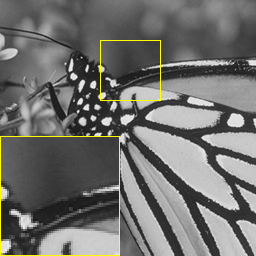
\includegraphics[width=0.18\linewidth]{2-9-1}  
	}\hspace{-0.02\linewidth}
	\subfigure[noisy image/20.17dB]{   
		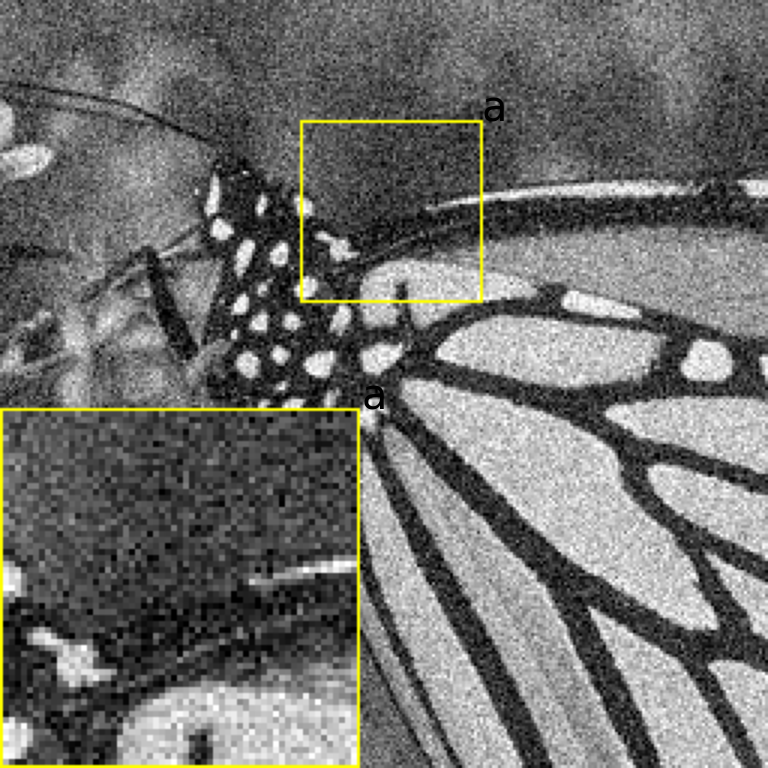
\includegraphics[width=0.18\linewidth]{2-9-2}  
	}\hspace{-0.02\linewidth}
	\subfigure[BM3D/29.39dB]{   
		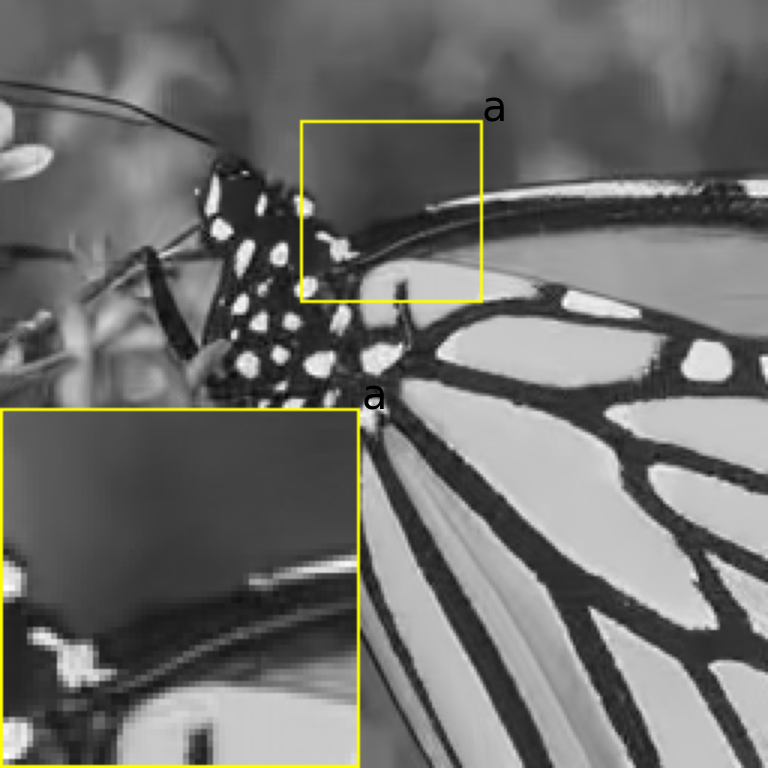
\includegraphics[width=0.18\linewidth]{2-9-3}  
	} 
	\\
	\subfigure[DnCNN-S/\color{red}30.39dB]{   
		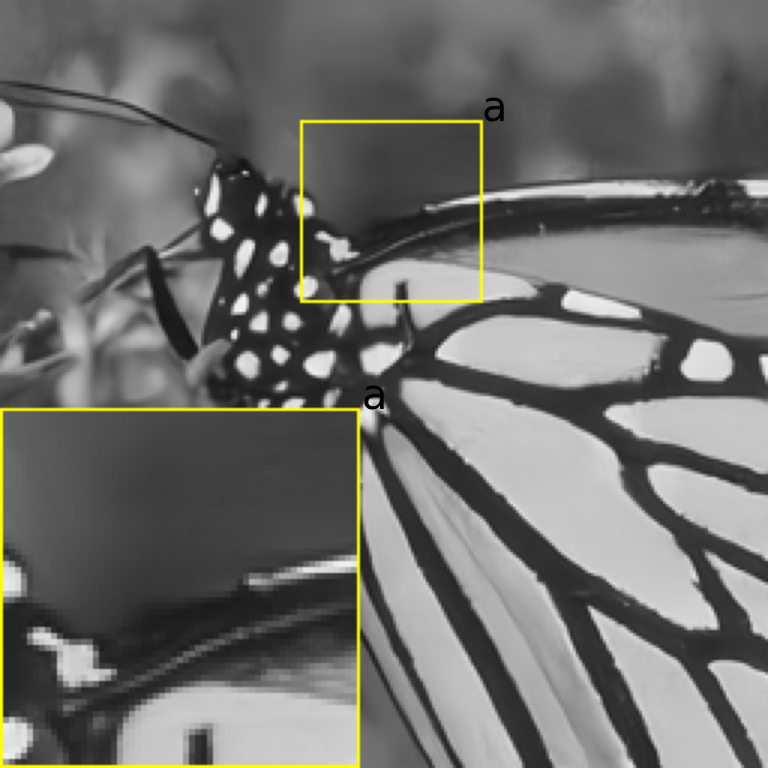
\includegraphics[width=0.18\linewidth]{2-9-4}  
	}\hspace{-0.02\linewidth}
	\subfigure[DnCNN-B/30.38dB]{   
		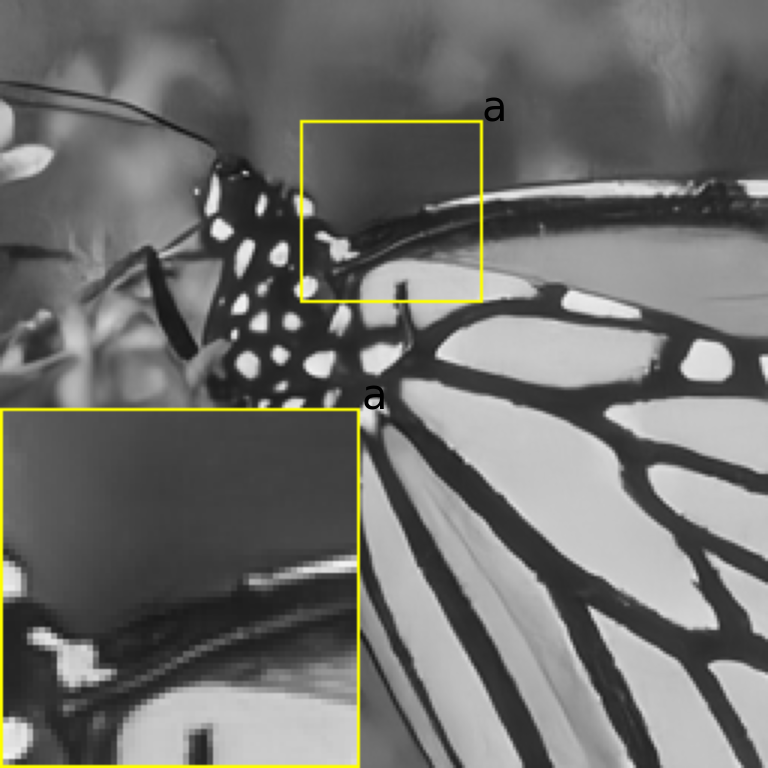
\includegraphics[width=0.18\linewidth]{2-9-5}  
	}\hspace{-0.02\linewidth}
	\subfigure[IRCNN-S/30.26dB]{   
		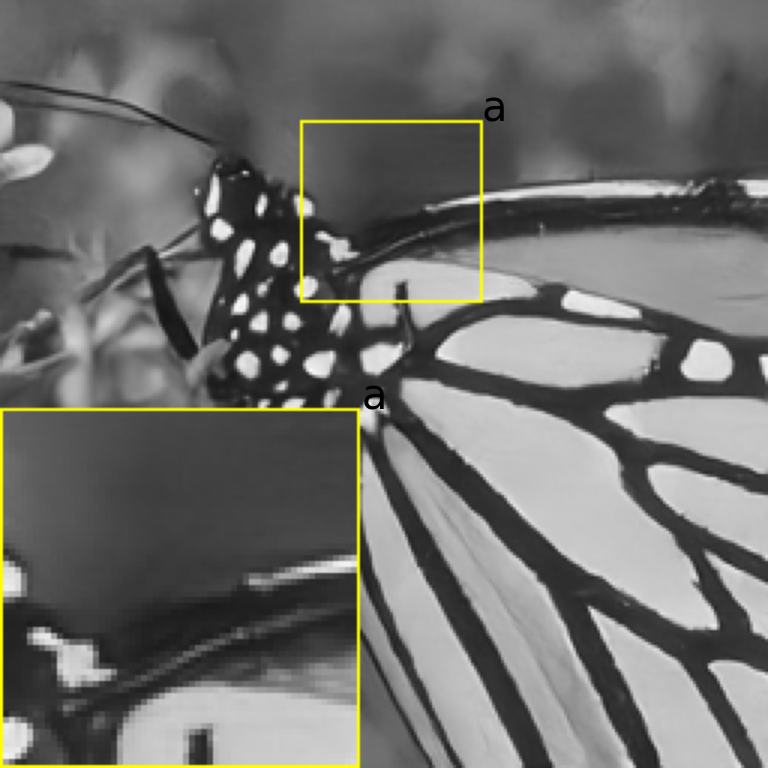
\includegraphics[width=0.18\linewidth]{2-9-6}  
	}\hspace{-0.02\linewidth}
	\subfigure[IRCNN-B/30.11dB]{   
		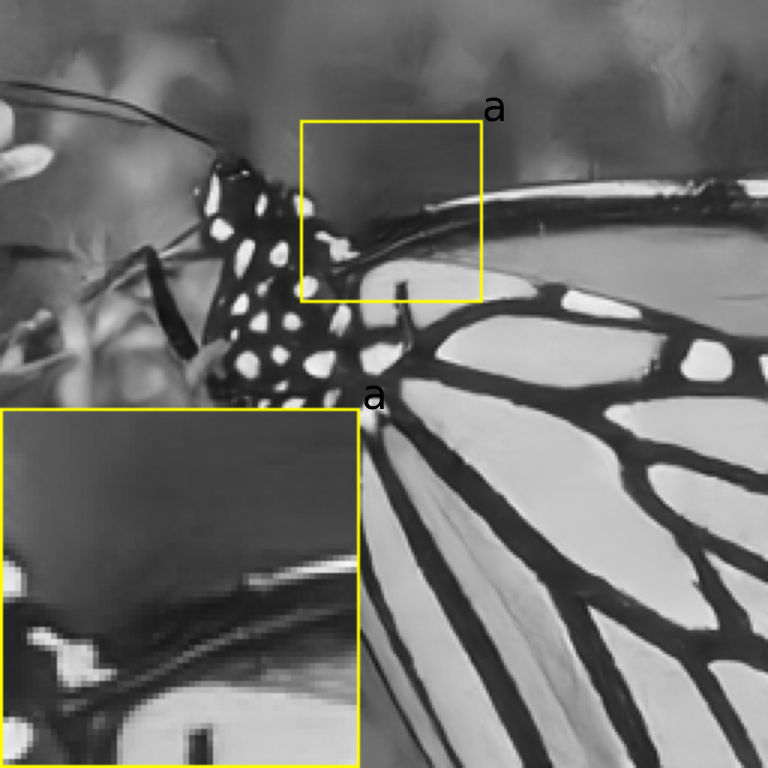
\includegraphics[width=0.18\linewidth]{2-9-7}  
	} 
	\caption{不同去噪算法的去噪效果图($\sigma=25$)} 
	\label{fig:2-9} 
\end{figure}
\begin{figure}[!htbp]
	\centering 
	\subfigure[original image]{
		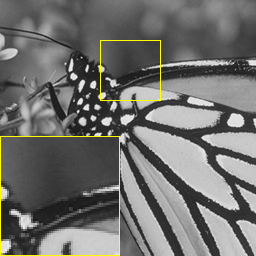
\includegraphics[width=0.18\linewidth]{2-10-1}  
	}\hspace{-0.02\linewidth}
	\subfigure[noisy image/20.17dB]{   
		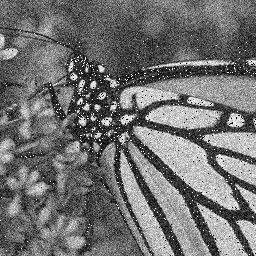
\includegraphics[width=0.18\linewidth]{2-10-2}  
	}\hspace{-0.02\linewidth}
	\subfigure[BM3D/29.39dB]{   
		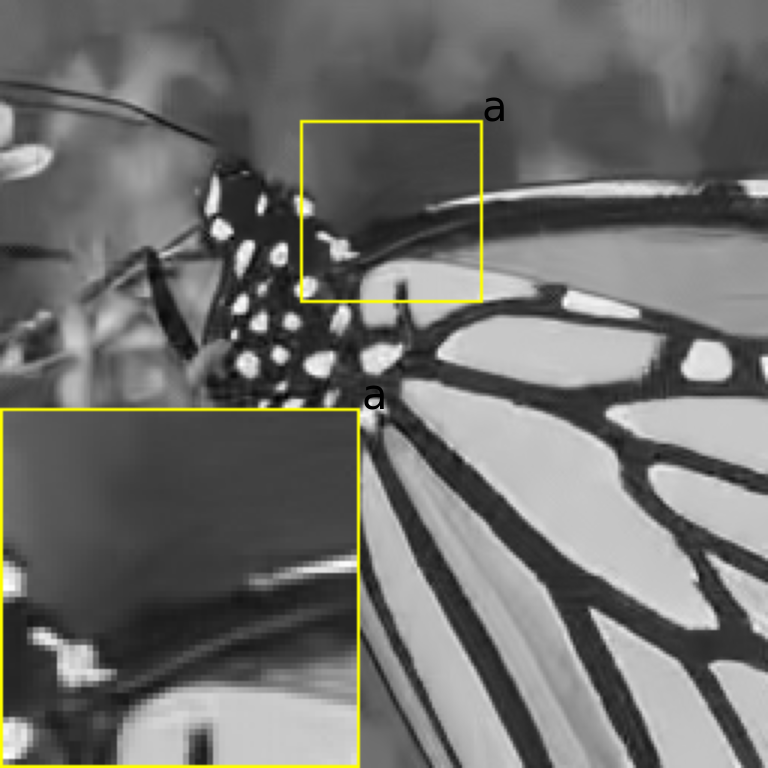
\includegraphics[width=0.18\linewidth]{2-10-3}  
	} 
	\\
	\subfigure[\tiny{realSN-DnCNN-S/30.37dB}]{   
		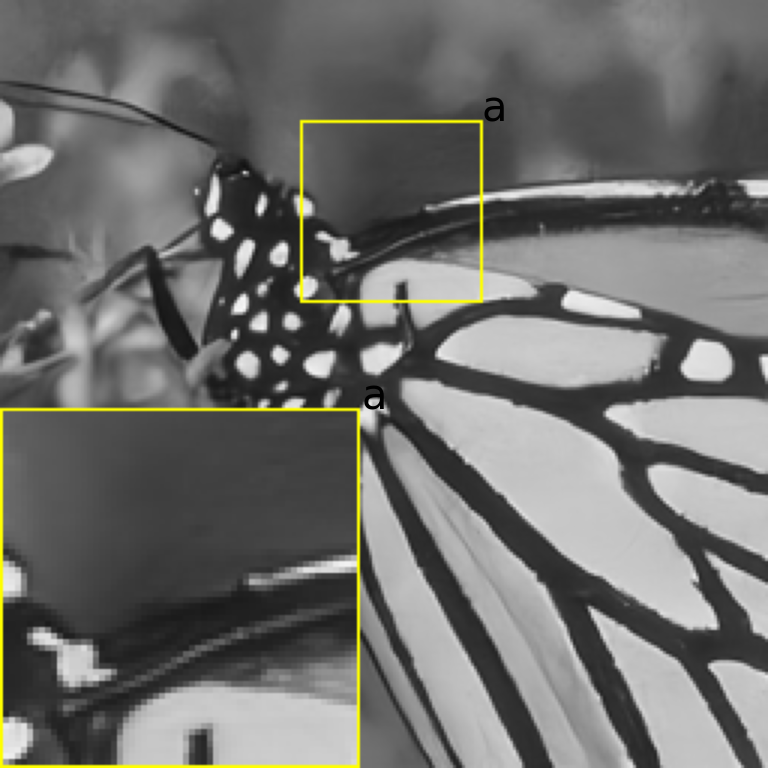
\includegraphics[width=0.18\linewidth]{2-10-4}  
	}\hspace{-0.02\linewidth}			
	\subfigure[\tiny{realSN-DnCNN-B/\color{red}30.38dB}]{   
		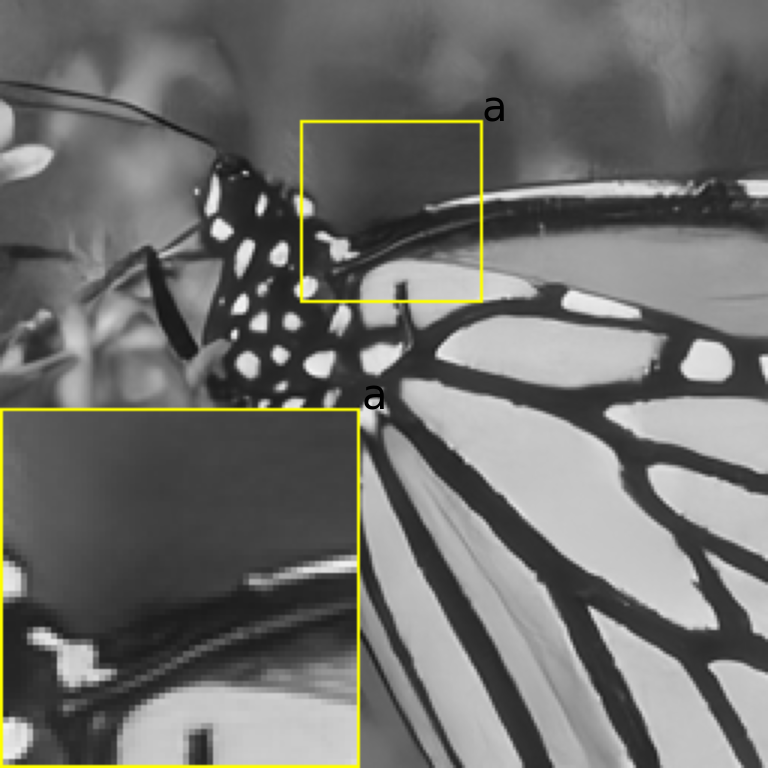
\includegraphics[width=0.18\linewidth]{2-10-5}  
	}\hspace{-0.02\linewidth}			
	\subfigure[\tiny{realSN-IRCNN-S/30.29dB}]{   
		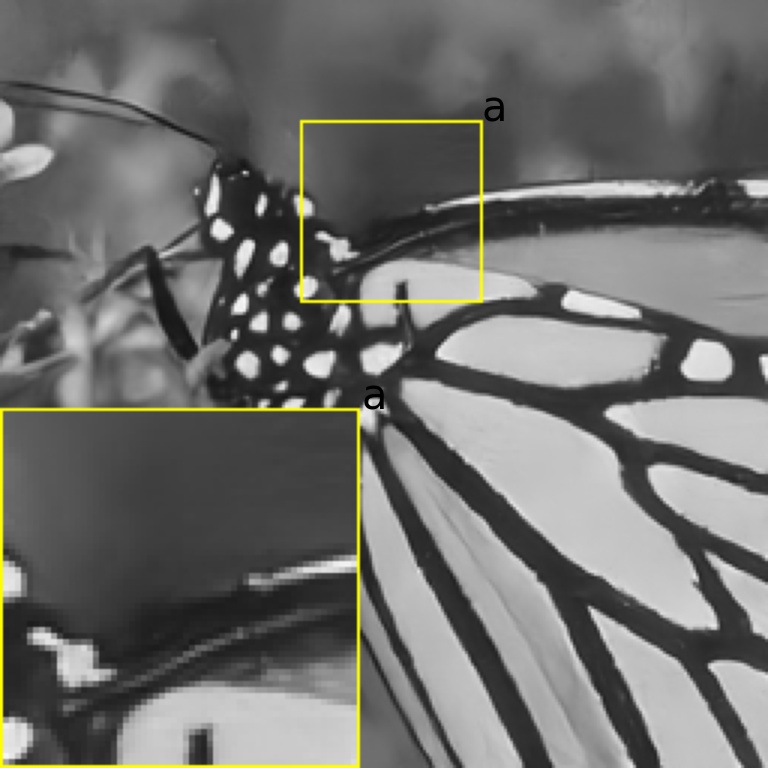
\includegraphics[width=0.18\linewidth]{2-10-6}  
	}\hspace{-0.02\linewidth}			
	\subfigure[\tiny{realSN-IRCNN-B/30.07dB}]{   
		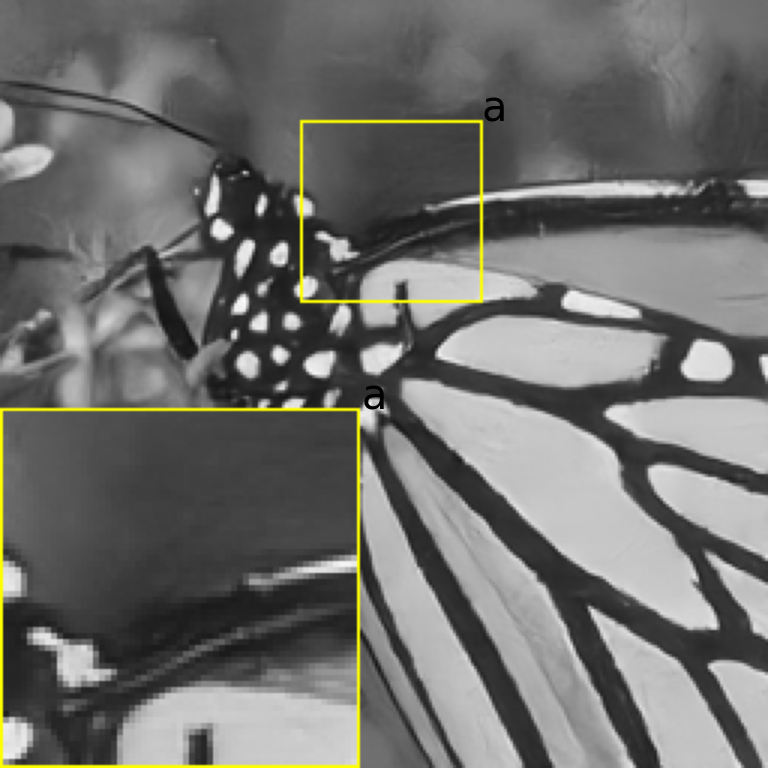
\includegraphics[width=0.18\linewidth]{2-10-7}
	}
	\caption{实谱归一化不同去噪算法的去噪效果图($\sigma=25$)}
	\label{fig:2-10}  
\end{figure}

从图\ref{fig:2-9}与图\ref{fig:2-10}可以出:(1)横向对比,从主观视觉的角度已无法区分各去噪图像的优劣,但基于深度学习的去噪算法在PSNR/SSIM上高于传统的BM3D算法,表明深度学习技术对于图像去噪任务的潜在优势,利用深度神经网络构造的去噪器取得当前SOTA结果;(2)纵向对比,基于实谱归一化的深度学习去噪器并未增强对盲高斯噪声的泛化能力,去噪效果与未加实谱归一化的原始去噪算法相当,引起这一现象原因为利普希茨约束导致欠拟合。因为神经网络利普希茨常数的估计较为复杂,现存的方法存在缺乏准确性或可伸缩性差等缺点,无法有效接近真实的全局利普希茨常数,只能在局部进行估计\supercite{Fazlyab}。故暂时无法确定实谱归一化是否真的起到了限制深度神经网络利普希茨常数的作用,留作日后研究。
%\begin{figure}[!hptb]
%	\centering
%	\begin{minipage}[t]{0.5\linewidth}
%		\centering
%		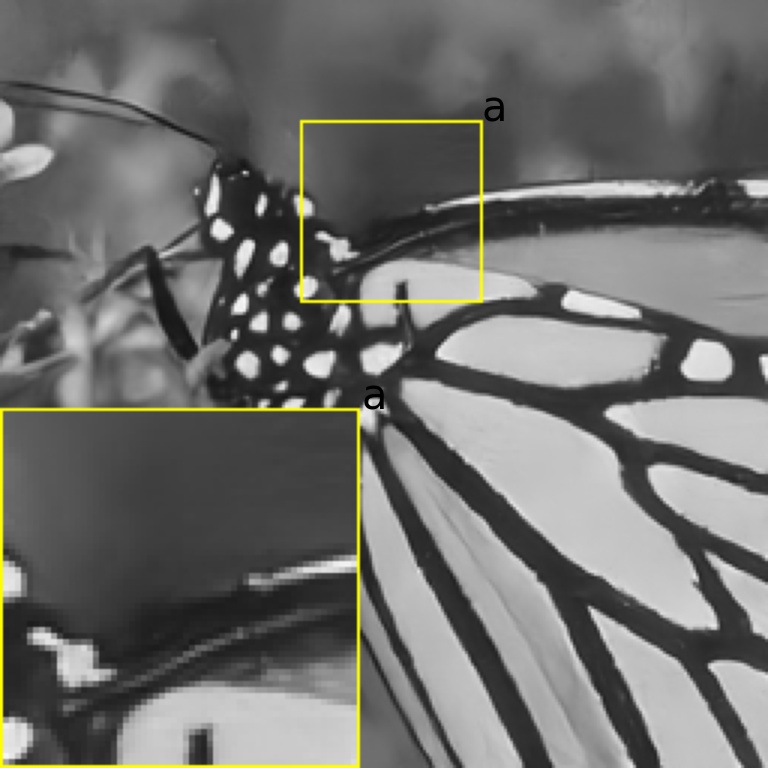
\includegraphics[width=\textwidth]{2-10-6}
%		\caption{text}
%	\end{minipage}%
%	\begin{minipage}[t]{0.5\textwidth}
%		\centering
%		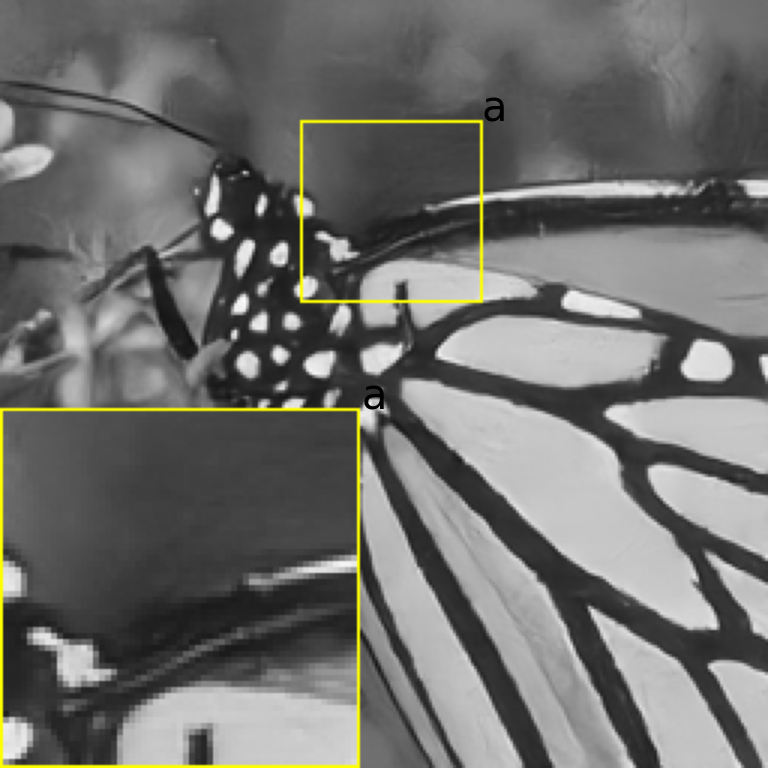
\includegraphics[width=\textwidth]{2-10-7}
%	\end{minipage}
%	\caption{两个并排图形}\label{fig-dbfig}
%\end{figure}

\subsection{TACE及其对比算法参数设置}
本章采用的测试数据集TestImages来自文献[10],共包含六张自然图像与六张非自然图像。在编码衍射系统设置中,本章采用随机空间光调制掩膜$M_i$,即复平面单位圆的随机均匀抽样,其如图\ref{fig:3-4}所示。此时它对应的观测矩阵为$A_{i}=FM_i,i\in[1,2,3,4]$,其中$F$表示二维快速傅里叶变换。故编码衍射模型表示为:
\begin{equation} \label{equation:3-22}
	y=\vert{Ax}\vert+\omega.
\end{equation}
其中$\omega$表示随机噪声。
\begin{figure}[!htbp]
	\centering
	\subfigure[$M_1$]{
		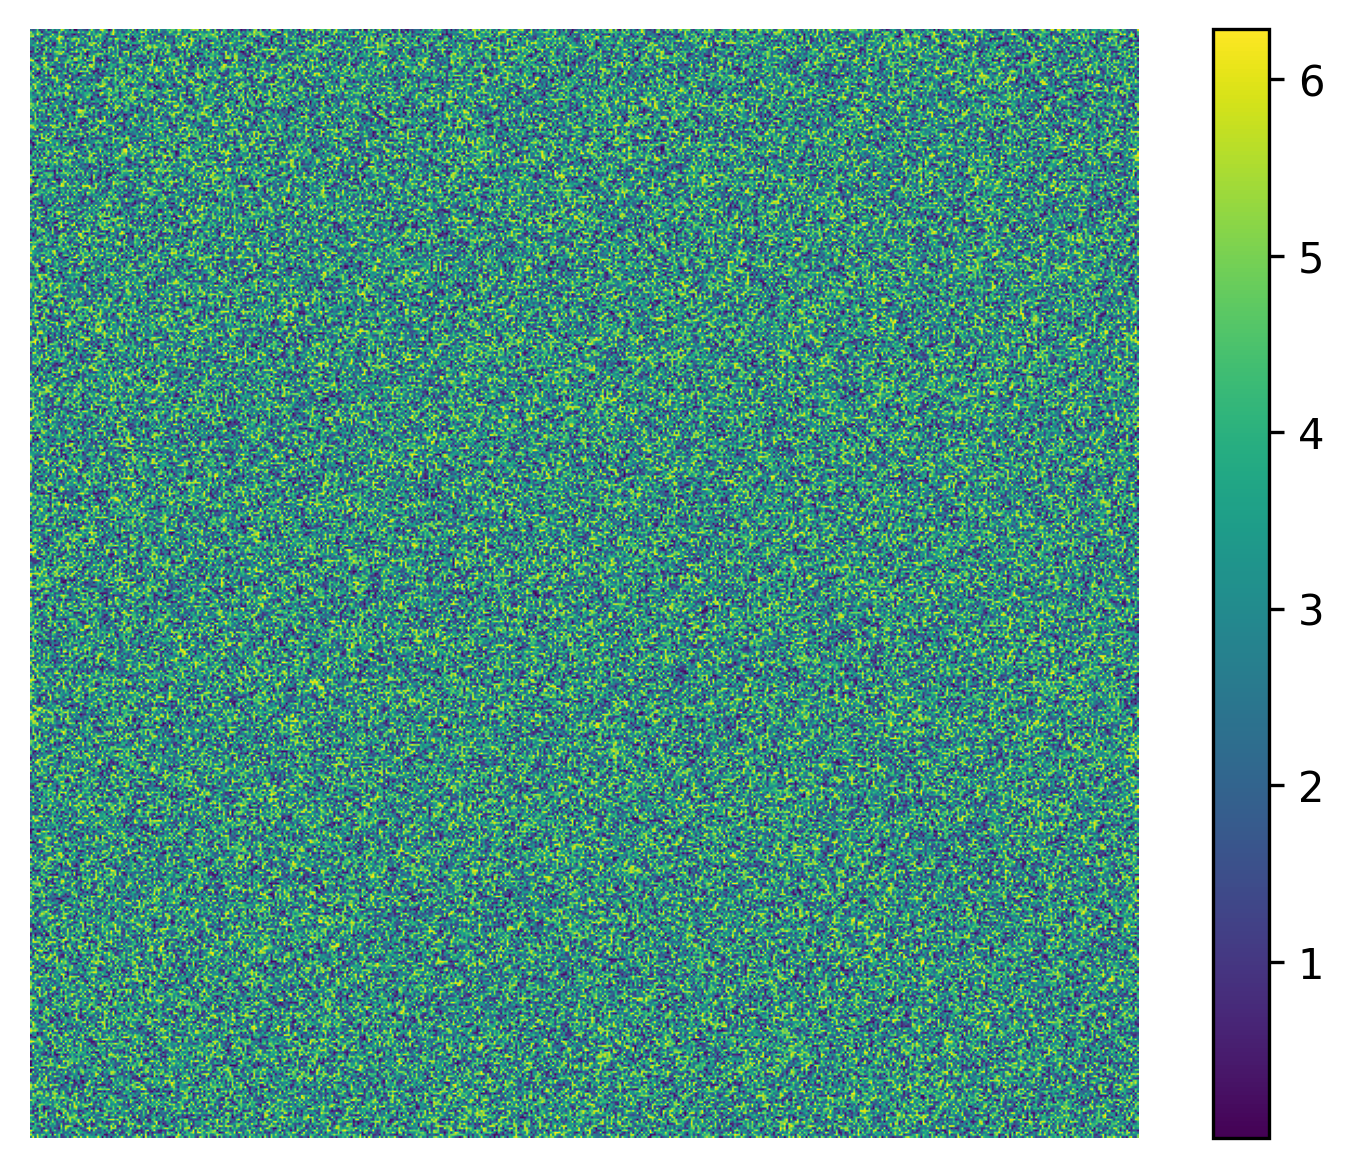
\includegraphics[width=0.2\linewidth]{barbara_slm_1}
	}\hspace{-0.0\linewidth}
	\subfigure[$M_2$]{
		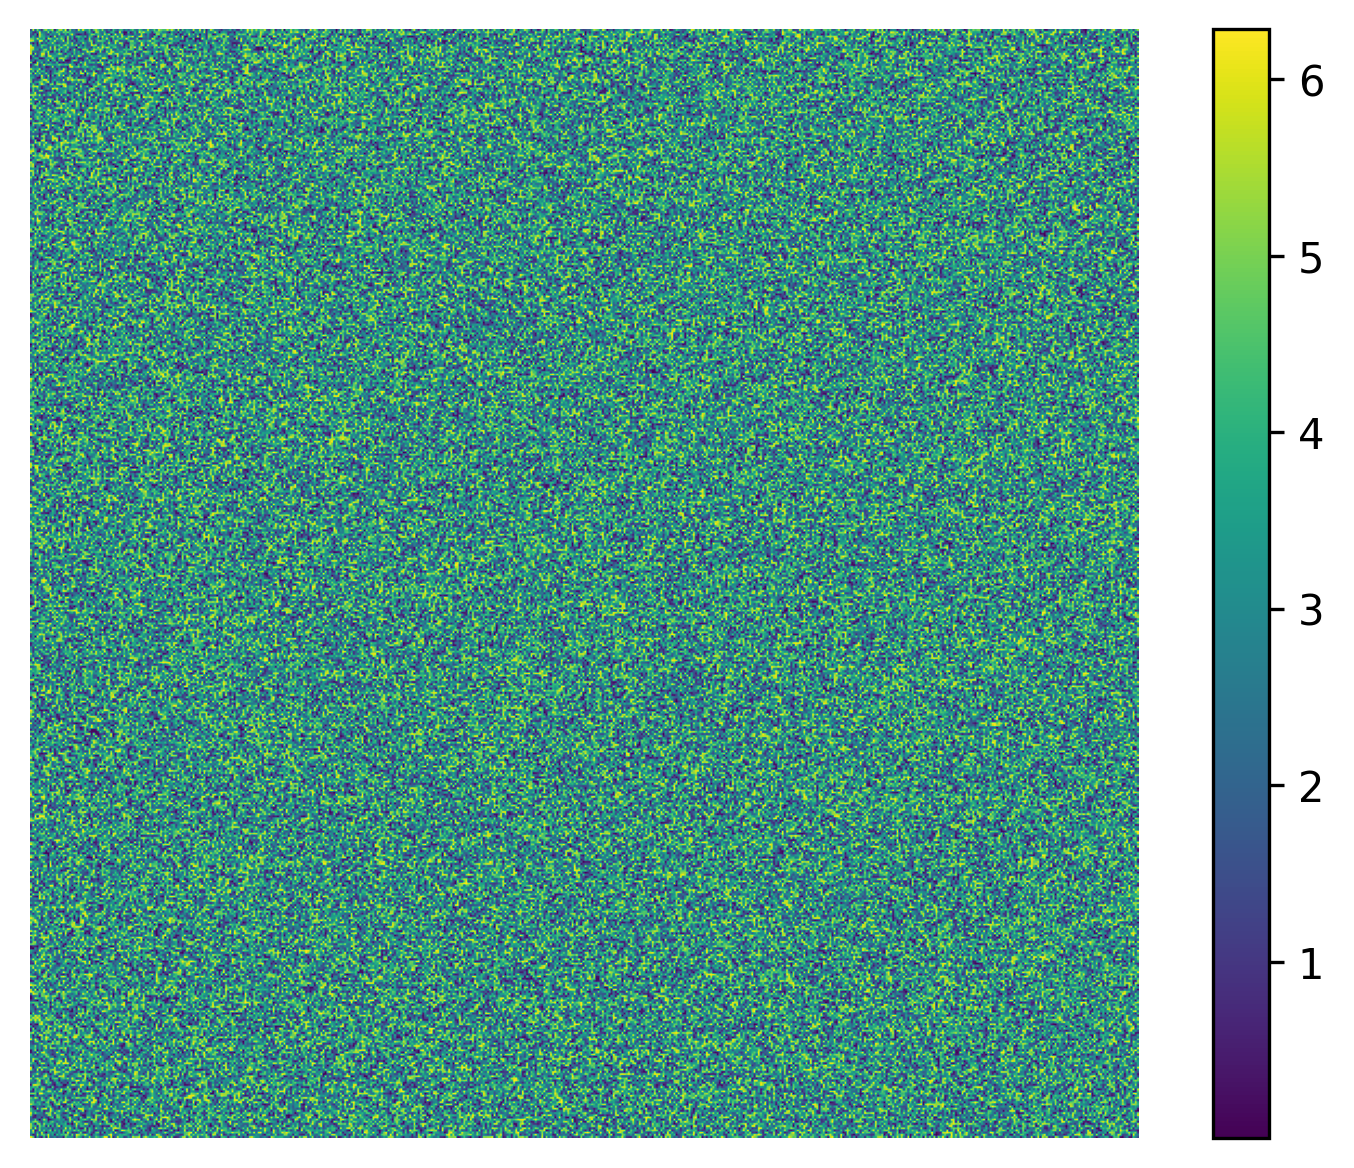
\includegraphics[width=0.2\linewidth]{barbara_slm_2}
	}\hspace{-0.0\linewidth}
	\subfigure[$M_3$]{
		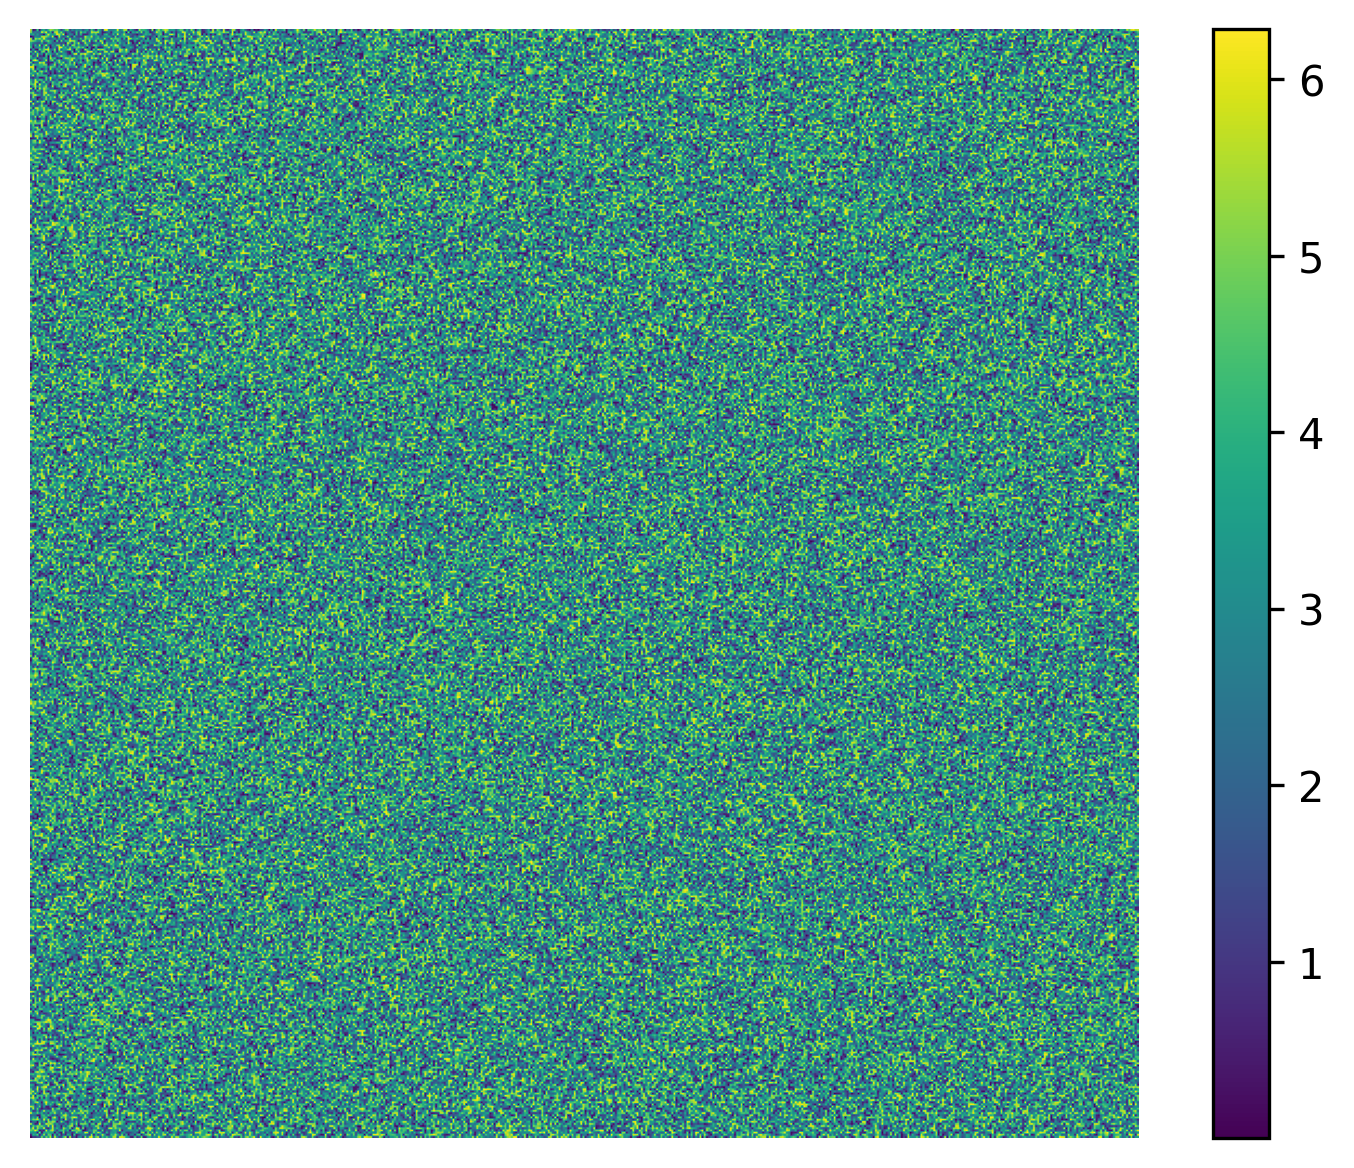
\includegraphics[width=0.2\linewidth]{barbara_slm_3}
	}\hspace{-0.0\linewidth}
	\subfigure[$M_4$]{
		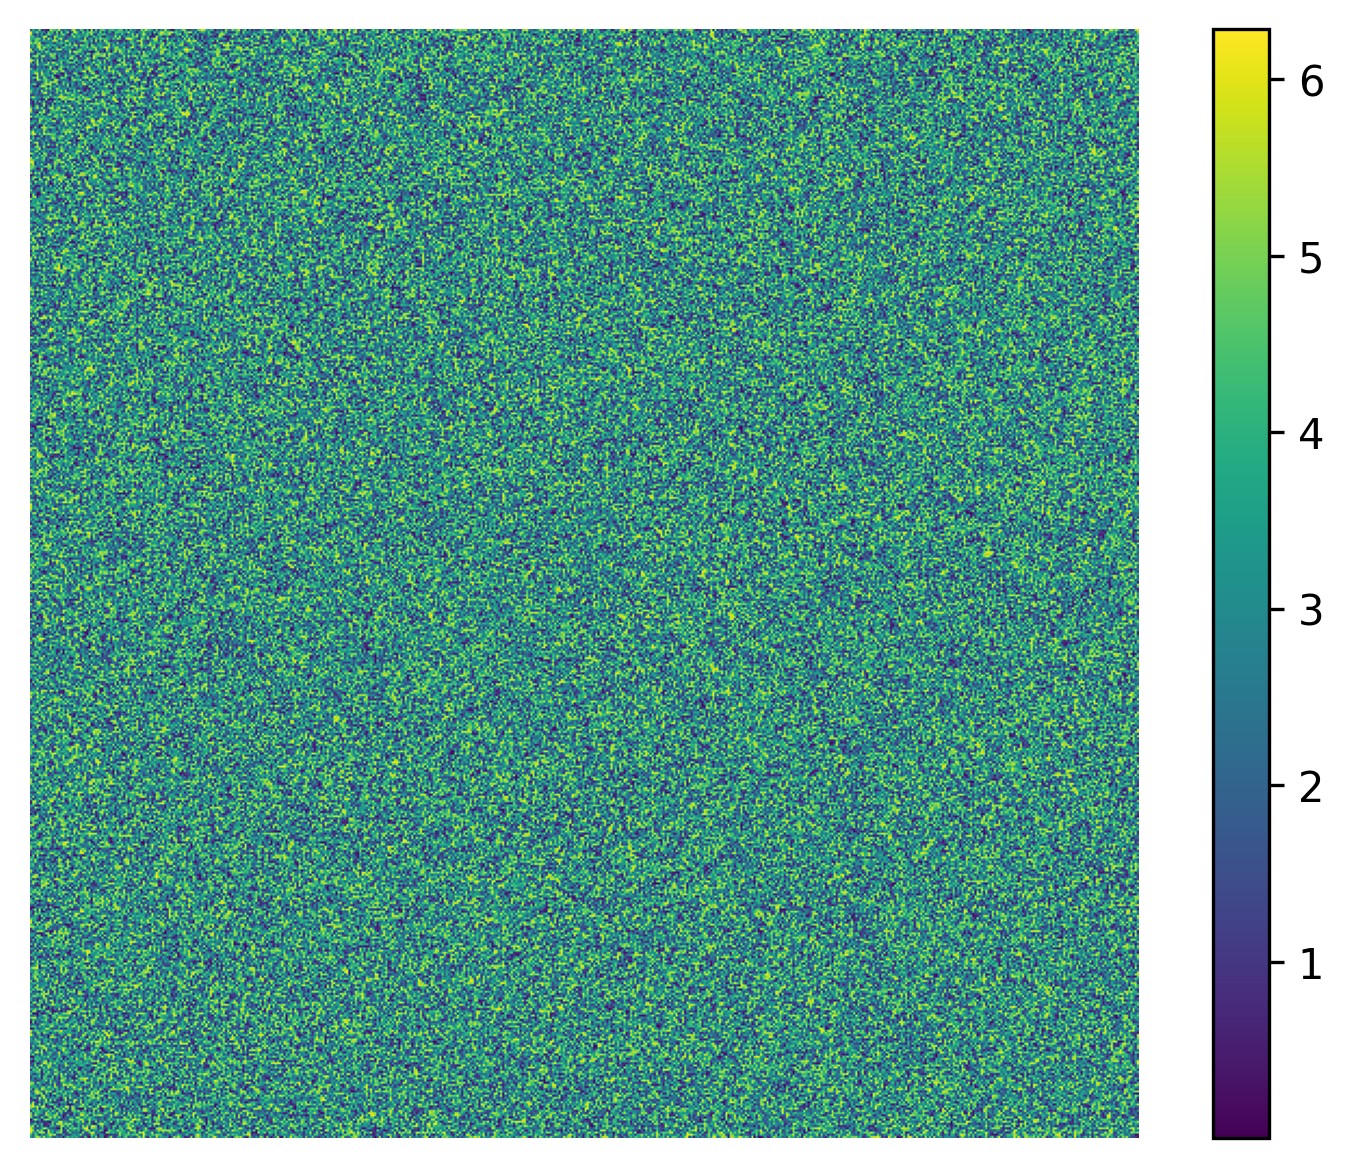
\includegraphics[width=0.2\linewidth]{barbara_slm_4}
	}
	\caption{Phase-only SLM示意图}
	\label{fig:3-4}
\end{figure}

在以下所有仿真实验中,随机SLM均设置相同的随机种子,以保证输入测试用例一致。此外,为了验证本文算法的有效性,本章针对不同噪声类型与噪声水平的观测值进行相位恢复仿真实验,并且从PSNR、SSIM和主观视觉角度对所提算法及其对比算法进行客观评价。

为了保证对比的公平性,算法\ref{algorithm:3-1}、\ref{algorithm:3-2}、\ref{algorithm:3-3}与peDeep均采用同一盲去噪器($\sigma=1\sim{50}$)。算法\ref{algorithm:3-1}、\ref{algorithm:3-2}、\ref{algorithm:3-3}根据默认值设置参数,prDeep利用FASTA的默认设置。另外,所有算法的初始值服从均匀分布。

\subsection{抗高斯噪声模型}
当式\eqref{equation:3-22}中的$\omega\sim{\mathcal{N}(0,\sigma^2\mathbf{I})}$时,观测值受高斯噪声的污染。相应的信噪比(SNR)定义为:
\begin{equation} \label{equation:3-23}
	\text{SNR}(\hat{y},y)=20\log_{10}{\frac{\Vert{y}\Vert_2}{\Vert{y-\hat{y}}\Vert_2}}.
\end{equation}
其中$\hat{y}$表示含噪观测值,$y$表示真实图像。表\ref{table:3-4}与表\ref{table:3-5}给出了不同噪声强度、不同去噪算子下四种算法重构原始图像的PSNR/SSIM结果。
\begin{table}[!htbp]
	\def\arraystretch{1.4}\centering\zihao{5}
	\caption{不同算法在DnCNN下获得平均PSNR(dB)/SSIM比较}
	\label{table:3-4}
	\begin{tabular*}{\linewidth}{@{}@{\extracolsep{\fill}}ccccc@{}}
		\toprule	%\multirow{2}*{算法}
		算法	& prDeep & PnP-ADMM & PnP-FBS & TACE \\
		%\cmidrule(r){2-5}
		\midrule
		$\text{SNR}=15$        & 32.37/0.8426   & 34.29/0.9003  & {\color{red}34.40}/0.8939 & 34.31/{\color{red}0.9005}  \\
		$\text{SNR}=20$        & 33.39/0.8387   &37.00/{\color{red}0.9392}  &{\color{red}37.11}/0.9345 & 36.98/0.9383  \\
		$\text{SNR}=25$        & 36.00/0.8907   & 39.60/{\color{red}0.9588}  & {\color{red}39.70}/0.9581 & 39.55/0.9567  \\
		\bottomrule
	\end{tabular*}
\end{table}
\begin{table}[!htbp]
	\def\arraystretch{1.4}\centering\zihao{5}
	\caption{不同算法在IRCNN下获得平均PSNR(dB)/SSIM比较}
	\label{table:3-5}
	\begin{tabular*}{\linewidth}{@{}@{\extracolsep{\fill}}ccccc@{}}
		\toprule
		算法	& prDeep & PnP-ADMM & PnP-FBS & TACE \\ %\cmidrule(r){2-5}
		\midrule
		$\text{SNR}=15$        & 32.25/0.8504   & 33.93/0.9050  & {\color{red}34.10}/{\color{red}0.9065} & 33.93/0.9035  \\
		$\text{SNR}=20$        & 33.20/0.8380   & 36.50/0.9364  & {\color{red}36.70}/{\color{red}0.9374} & 36.47/0.9347  \\
		$\text{SNR}=25$        & 35.99/0.8906   & 39.00/0.9562  & {\color{red}39.22}/{\color{red}0.9563} & 38.92/0.9531  \\
		\bottomrule
	\end{tabular*}
\end{table}

从表\ref{table:3-4}与表\ref{table:3-5}可以看出,TACE算法的重构图像质量优于prDeep算法,并且与PnP-ADMM算法结果接近,验证了PnP-ADMM与TACE收敛到相同的不动点。由于PnP-FBS使用了自适应迭代步长技术,使得该算法为SOTA结果。再者TACE算法有着明确的优化方程,故在理论上可以分析其收敛性与收敛速度。而PnP-ADMM和PnP-FBS没有明确的优化问题,为非凸框架,分析收敛性依赖于对去噪算子的假设。

为衡量算法的计算复杂度,表\ref{table:3-6}给出了四种算法在同一测试集上的GPU平均运行时间。从表\ref{table:3-6}可以看出TACE算法的运行时间与即插即用算法比较接近,并没有出现过大的数量级差距。并且这是算法的绝对运行时间,可比较性存在争议。
\begin{table}[!htbp]
	\def\arraystretch{1.4}\centering\zihao{5}
	\caption{不同算法不同去噪器在Barbara上的运行时间(s)(SNR=25dB)}
	\label{table:3-6}
	\begin{tabular*}{\linewidth}{@{}@{\extracolsep{\fill}}ccccc@{}}
		\toprule
		算法	& prDeep & PnP-ADMM & PnP-FBS & TACE \\ %\cmidrule(r){2-5}
		\midrule
	    512x512 & 27.92/{\color{blue}8.70}   & {\color{blue}25.74}/9.64  & 28.43/9.46 & 30.56/10.58 \\
	    Device	         & GPU   & GPU  & GPU	& GPU \\
		\bottomrule
	\end{tabular*}
\end{table}

图\ref{fig:3-6}与图\ref{fig:3-7}给出了不同算法在DnCNN和IRCNN去噪算子下当SNR=15dB时Barbara与Pollen的重构结果。从图\ref{fig:3-6}与图\ref{fig:3-7}可以看出TACE算法与对比算法已经无法从主观视觉上区别重构图像的优劣。但在PSNR的角度,两阶段TACE算法并没有取得SOTA的结果,这是因为TACE算法与PnP-ADMM算法不动点的等价性。
\begin{figure}[!htbp]
	\centering
	\subfigure[Original]{
		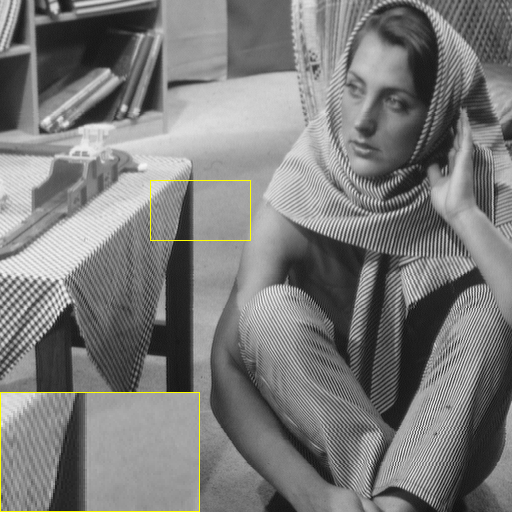
\includegraphics[width=0.18\linewidth]{3-6-1}
	}\hspace{-0.01\linewidth}
	\subfigure[prDeep/31.10]{
		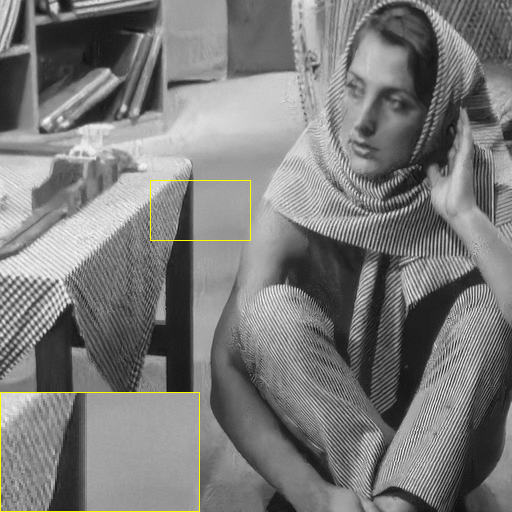
\includegraphics[width=0.18\linewidth]{3-6-2}
	}\hspace{-0.01\linewidth}
	\subfigure[PnP-ADMM/31.36]{
		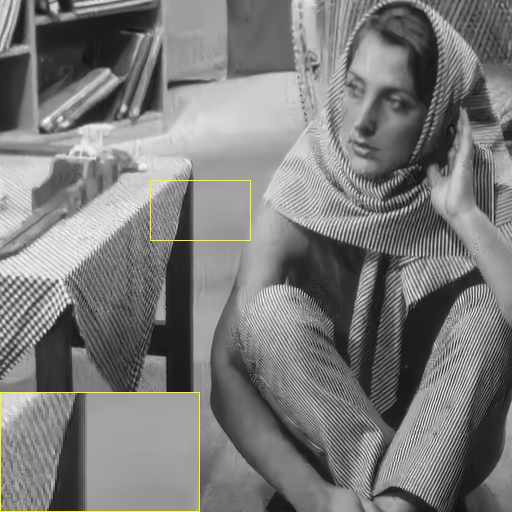
\includegraphics[width=0.18\linewidth]{3-6-3}
	}\hspace{-0.01\linewidth}
	\subfigure[PnP-FBS/{\color{red}31.51}]{
		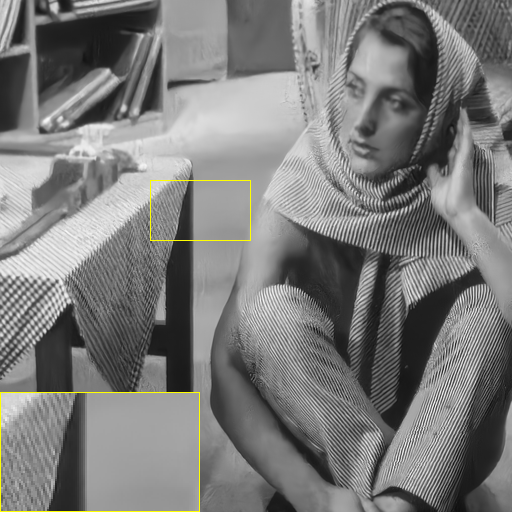
\includegraphics[width=0.18\linewidth]{3-6-4}
	}\hspace{-0.01\linewidth}
	\subfigure[TACE/31.43]{
		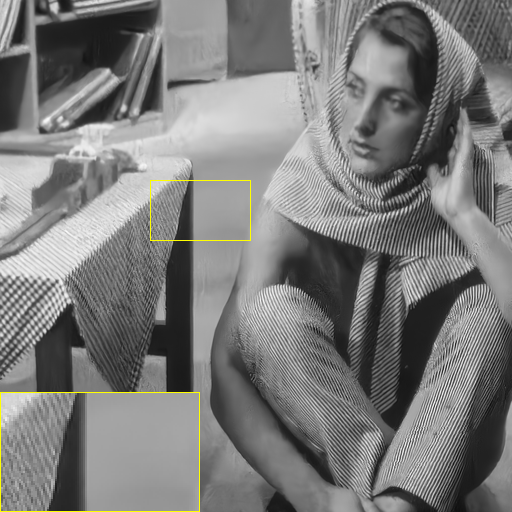
\includegraphics[width=0.18\linewidth]{3-6-5}
	}
	
	\subfigure[Original]{
		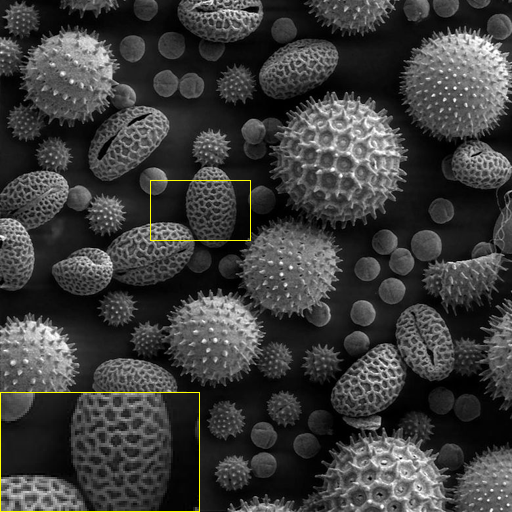
\includegraphics[width=0.18\linewidth]{3-6-6}
	}\hspace{-0.01\linewidth}
	\subfigure[prDeep/31.24]{
		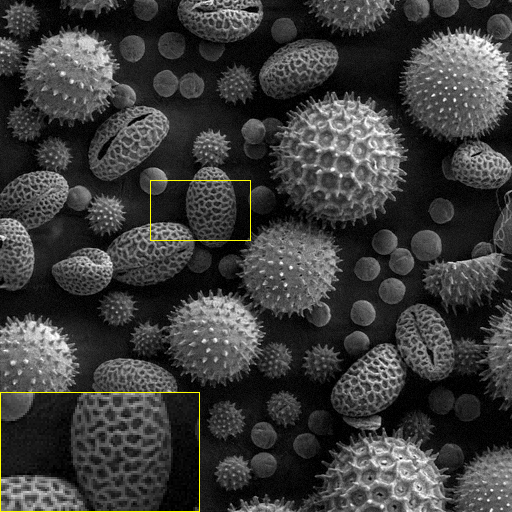
\includegraphics[width=0.18\linewidth]{3-6-7}
	}\hspace{-0.01\linewidth}
	\subfigure[PnP-ADMM/32.90]{
		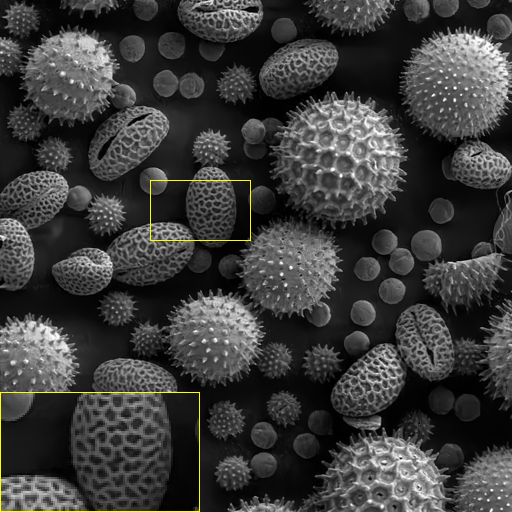
\includegraphics[width=0.18\linewidth]{3-6-8}
	}\hspace{-0.01\linewidth}
	\subfigure[PnP-FBS/{\color{red}33.01}]{
		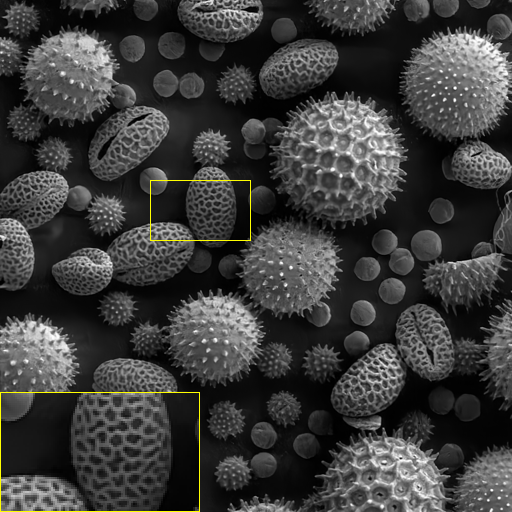
\includegraphics[width=0.18\linewidth]{3-6-9}
	}\hspace{-0.01\linewidth}
	\subfigure[TACE/32.92]{
		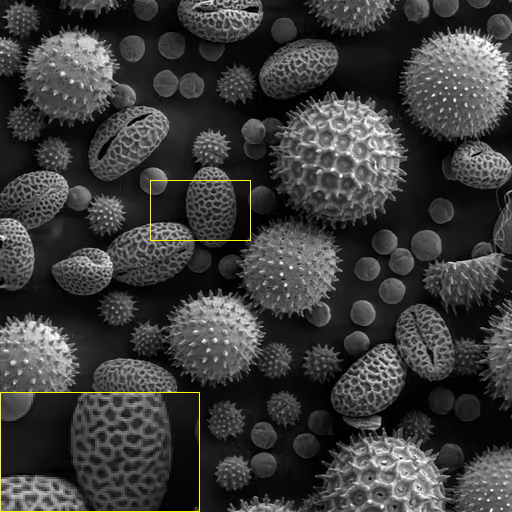
\includegraphics[width=0.18\linewidth]{3-6-10}
	}
	\caption{Barbara与Pollen重构结果(SNR=15dB,DnCNN)} 
	\label{fig:3-6}
\end{figure}
\begin{figure}[!htbp]
	\centering
	\subfigure[Original]{
		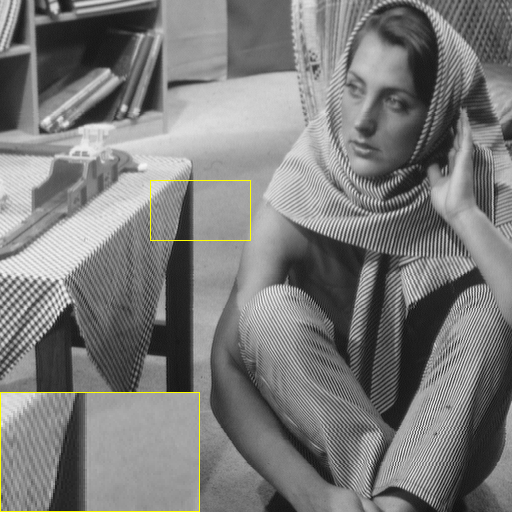
\includegraphics[width=0.18\linewidth]{3-7-1}
	}\hspace{-0.01\linewidth}
	\subfigure[prDeep/30.38]{
		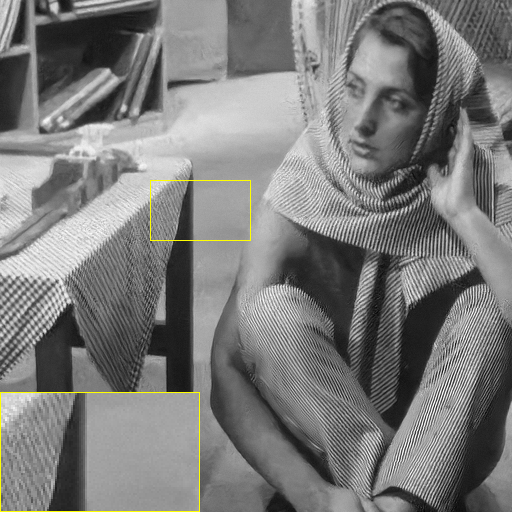
\includegraphics[width=0.18\linewidth]{3-7-2}
	}\hspace{-0.01\linewidth}
	\subfigure[PnP-ADMM/30.55]{
		\includegraphics[width=0.18\linewidth]{3-7-3}
	}\hspace{-0.01\linewidth}
	\subfigure[PnP-FBS/{\color{red}31.00}]{
		\includegraphics[width=0.18\linewidth]{3-7-4}
	}\hspace{-0.01\linewidth}
	\subfigure[TACE/30.60]{
		\includegraphics[width=0.18\linewidth]{3-7-5}
	}
	
	\subfigure[Original]{
		\includegraphics[width=0.18\linewidth]{3-7-6}
	}\hspace{-0.01\linewidth}
	\subfigure[prDeep/30.96]{
		\includegraphics[width=0.18\linewidth]{3-7-7}
	}\hspace{-0.01\linewidth}
	\subfigure[PnP-ADMM/32.56]{
		\includegraphics[width=0.18\linewidth]{3-7-8}
	}\hspace{-0.01\linewidth}
	\subfigure[PnP-FBS/{\color{red}32.72}]{
		\includegraphics[width=0.18\linewidth]{3-7-9}
	}\hspace{-0.01\linewidth}
	\subfigure[TACE/32.58]{
		\includegraphics[width=0.18\linewidth]{3-7-10}
	}
	\caption{Barbara与Pollen重构结果(SNR=15dB,IRCNN)}
	\label{fig:3-7}
\end{figure}

为验证假设\ref{assumption:3-2},图\ref{fig:3-8}给出了PnP-ADMM与TACE算法各个代理在迭代过程中的利普希茨常数分布直方图,测试图像为Barbara,SNR=15dB,各个代理迭代过程中的利普希茨常数由定义\ref{def:3-1}计算。
\begin{figure}[!htbp]
	\centering
	\subfigure[\scriptsize PnP-ADMM(DnCNN)]{
		\label{subfigure:3-1-1}
		\begin{minipage}[b]{0.18\linewidth}
			\centering
			\includegraphics[width=\linewidth]{3-8-1}\\
			\includegraphics[width=\linewidth]{3-8-2}
			%\caption{fig}
		\end{minipage}
	}
	\subfigure[\scriptsize TACE(DnCNN)]{
		\label{subfigure:3-1-2}
		\begin{minipage}[b]{0.18\linewidth}
			\centering
			\includegraphics[width=\linewidth]{3-8-3}\\
			\includegraphics[width=\linewidth]{3-8-4}
			%\caption{fig}
		\end{minipage}
	}
	\subfigure[\scriptsize PnP-ADMM(IRCNN)]{
		\label{subfigure:3-1-3}
		\begin{minipage}[b]{0.18\linewidth}
			\centering
			\includegraphics[width=\linewidth]{3-8-5}\\
			\includegraphics[width=\linewidth]{3-8-6}
			%\caption{fig}
		\end{minipage}
	}
	\subfigure[\scriptsize TACE(IRCNN)]{
		\label{subfigure:3-1-4}
		\begin{minipage}[b]{0.18\linewidth}
			\centering
			\includegraphics[width=\linewidth]{3-8-7}\\
			\includegraphics[width=\linewidth]{3-8-8}
			%\caption{fig}
		\end{minipage}
	}
	\subfigure[\scriptsize PnP-FBS]{
		\label{subfigure:3-1-5}
		\begin{minipage}[b]{0.18\linewidth}
			\centering
			\includegraphics[width=\linewidth]{3-8-9}\\
			\includegraphics[width=\linewidth]{3-8-10}
			%\caption{fig}
		\end{minipage}
	}
	\caption{PnP-ADMM与TACE算法在迭代过程中的利普希茨常数分布直方图}
	\label{fig:3-8}
\end{figure}

图\ref{fig:3-8}中的\subref{subfigure:3-1-1}、\subref{subfigure:3-1-2}分别表示PnP-ADMM算法、TACE算法中数据保真项近邻算子与DnCNN去噪器在迭代过程中的利普希茨常数统计直方图;\subref{subfigure:3-1-3}、\subref{subfigure:3-1-4}分别表示PnP-ADMM算法、TACE算法中数据保真项近邻算子与IRCNN去噪器在迭代过程中的利普希茨常数统计直方图;\subref{subfigure:3-1-5}表示PnP-FBS在迭代过程中的利普希茨常数统计直方图,上层为DnCNN,下层为IRCNN;除\subref{subfigure:3-1-5}外上层代表数据保真项的近邻算子,下层代表图像去噪算子。从图\ref{fig:3-8}可以看出,在迭代过程中,盲DnCNN和IRCNN去噪算子满足利普希茨约束假设,而编码衍射模型的非凸数据保真项的近邻算子却不是非扩张算子,不满足假设\ref{assumption:3-2}。故该算法无法保证收敛到不动点,关于数据保真项的求解算法有待进一步研究。

\subsection{抗泊松噪声模型}
当式\eqref{equation:3-20}中的$\omega\sim{\mathcal{N}(0,\alpha\vert{Ax}\vert)}$时,观测值受泊松噪声的污染。表\ref{table:3-7}与表\ref{table:3-8}给出了不同噪声强度不同去噪算子下四种算法重构原始图像的PSNR/SSIM结果。
\begin{table}[!htbp]
	\def\arraystretch{1.4}\centering\zihao{5}
	\caption{不同算法在DnCNN下获得平均PSNR(dB)/SSIM比较}
	\label{table:3-7}
	\begin{tabular*}{\linewidth}{@{}@{\extracolsep{\fill}}cccccc@{}}
		\toprule
		算法 & prDeep & PnP-ADMM & PnP-FBS & TACE & 文献\cite{Kaixuan}\\ %\cmidrule(r){2-6}
		\midrule
		$\alpha=9$        & 37.35/0.9188   & 40.27/{\color{red}0.9638}  & {\color{red}40.33}/0.9635 & 40.20/0.9607 & {\color{red}40.33}/-  \\
		$\alpha=27$        & 32.53/0.8296   & 34.95/{\color{red}0.9210}  & {\color{red}35.02}/0.9096 & 34.95/0.9206  & 33.90/-	\\
		$\alpha=81$        & 28.51/0.8100   & 28.23/0.8052  & {\color{red}28.54}/{\color{red}0.8121} & 28.29/0.8073  & 27.23/-	\\
		\bottomrule
	\end{tabular*}
\end{table}
\begin{table}[!htbp]
	\def\arraystretch{1.4}\centering\zihao{5}
	\caption{不同算法在IRCNN下获得平均PSNR(dB)/SSIM比较}
	\label{table:3-8}
	\begin{tabular*}{\linewidth}{@{}@{\extracolsep{\fill}}ccccc@{}}
		\toprule
		算法     & prDeep & PnP-ADMM & PnP-FBS & TACE\\ %\cmidrule(r){2-5}
		\midrule
		$\alpha=9$         & 37.34/0.9188   & 39.63/{\color{red}0.9619}  & {\color{red}39.78}/0.9613 & 39.55/0.9587\\
		$\alpha=27$        & 32.43/0.8325   & 34.64/0.9209  & {\color{red}34.83}/{\color{red}0.9220} & 34.63/0.9200\\
		$\alpha=81$        & 28.45/0.8214   & 28.32/0.8230  & {\color{red}28.49}/{\color{red}0.8245} & 28.23/0.8220\\
		\bottomrule
	\end{tabular*}
\end{table}

从表\ref{table:3-7}与表\ref{table:3-8}可以看出,TACE算法的重构图像质量高于peDeep算法,并且与PnP-ADMM算法结果接近,验证了PnP-ADMM与TACE收敛到相同的不动点。由于PnP-FBS使用了自适应迭代步长技术,使得该算法为SOTA结果。但是TACE算法在不同尺度泊松噪声下,对比文献\cite{Kaixuan}提出的基于强化学习的深度展开即插即用算法,PSNR的差值按泊松噪声污染强度由小到大依次为-0.13dB、1.05dB、1.06dB(TACE算法减去文献\cite{Kaixuan}所提的算法)。需要注意的是二者的观测矩阵不同。但通过二者较大的数值差距,可以看出TACE算法在泊松噪声强度较大的情况下优于文献\cite{Kaixuan}所提的算法。

为衡量算法的计算复杂度,本小节给出了算法的平均运行时间。表\ref{table:3-9}给出了四种算法在不同去噪算子下的GPU运行时间,关于平均运行时间的结论与上节高斯噪声的相同。
\begin{table}[!htbp]
	\def\arraystretch{1.4}\centering\zihao{5}
	\caption{不同算法不同去噪器在Barbara上的运行时间(s)($\alpha=81$)}
	\label{table:3-9}
	\begin{tabular*}{\linewidth}{@{}@{\extracolsep{\fill}}ccccc@{}}
		\toprule
		算法 & prDeep & PnP-ADMM & PnP-FBS & TACE	\\ %\cmidrule(r){2-5}
		\midrule
		512 x 512        & {\color{blue}27.78}/{\color{blue}9.15}   & 28.41/9.79  & 28.43/9.47 & 30.83/11.26\\
		Device	         & GPU   & GPU  & GPU 	& GPU \\
		\bottomrule
	\end{tabular*}
\end{table}

图\ref{fig:3-9}与图\ref{fig:3-10}给出了不同算法在DnCNN和IRCNN去噪算子下$\alpha=81$时Barbara与Pollen的重构结果,主观视觉结论与上节相同。
\begin{figure}[!htbp]
	\centering
	\subfigure[\scriptsize Original]{
		\includegraphics[width=0.18\linewidth]{3-9-1}
	}\hspace{-0.01\linewidth}
	\subfigure[\scriptsize prDeep/27.25]{
		\includegraphics[width=0.18\linewidth]{3-9-2}
	}\hspace{-0.01\linewidth}
	\subfigure[\scriptsize PnP-ADMM/26.80]{
		\includegraphics[width=0.18\linewidth]{3-9-3}
	}\hspace{-0.01\linewidth}
	\subfigure[\scriptsize PnP-FBS/{\color{red}27.26}]{
		\includegraphics[width=0.18\linewidth]{3-9-4}
	}\hspace{-0.01\linewidth}
	\subfigure[\scriptsize TACE/26.89]{
		\includegraphics[width=0.18\linewidth]{3-9-5}
	}

	\subfigure[\scriptsize Original]{
		\includegraphics[width=0.18\linewidth]{3-9-6}
	}\hspace{-0.01\linewidth}
	\subfigure[\scriptsize prDeep/25.80]{
		\includegraphics[width=0.18\linewidth]{3-9-7}
	}\hspace{-0.01\linewidth}
	\subfigure[\scriptsize PnP-ADMM/25.45]{
		\includegraphics[width=0.18\linewidth]{3-9-8}
	}\hspace{-0.01\linewidth}
	\subfigure[\scriptsize PnP-FBS/{\color{red}25.82}]{
		\includegraphics[width=0.18\linewidth]{3-9-9}
	}\hspace{-0.01\linewidth}
	\subfigure[\scriptsize TACE/25.55]{
		\includegraphics[width=0.18\linewidth]{3-9-10}
	}
	\caption{Barbara与Pollen重构结果($\alpha=81$,DnCNN)} 
	\label{fig:3-9}
\end{figure}
\begin{figure}[!htbp]
	\setlength{\belowcaptionskip}{-0.01\linewidth}
	\centering
	\subfigure[\scriptsize Original]{
		\includegraphics[width=0.18\linewidth]{3-10-1}
	}\hspace{-0.01\linewidth}
	\subfigure[\scriptsize prDeep/26.86]{
		\includegraphics[width=0.18\linewidth]{3-10-2}
	}\hspace{-0.01\linewidth}
	\subfigure[\scriptsize PnP-ADMM/26.54]{
		\includegraphics[width=0.18\linewidth]{3-10-3}
	}\hspace{-0.01\linewidth}
	\subfigure[\scriptsize PnP-FBS/{\color{red}26.88}]{
		\includegraphics[width=0.18\linewidth]{3-10-4}
	}\hspace{-0.01\linewidth}
	\subfigure[\scriptsize TACE/26.57]{
		\includegraphics[width=0.18\linewidth]{3-10-5}
	}

	\subfigure[\scriptsize Original]{
		\includegraphics[width=0.18\linewidth]{3-10-6}
	}\hspace{-0.01\linewidth}
	\subfigure[\scriptsize prDeep/25.80]{
		\includegraphics[width=0.18\linewidth]{3-10-7}
	}\hspace{-0.01\linewidth}
	\subfigure[\scriptsize PnP-ADMM/25.53]{
		\includegraphics[width=0.18\linewidth]{3-10-8}
	}\hspace{-0.01\linewidth}
	\subfigure[\scriptsize PnP-FBS/{\color{red}25.81}]{
		\includegraphics[width=0.18\linewidth]{3-10-9}
	}\hspace{-0.01\linewidth}
	\subfigure[\scriptsize TACE/25.61]{
		\includegraphics[width=0.18\linewidth]{3-10-10}
	}
	\caption{Barbara与Pollen重构结果($\alpha=81$,IRCNN)} 
	\label{fig:3-10}
\end{figure}

图\ref{fig:3-11}给出了PnP-ADMM与TACE算法中各个代理在迭代过程中的利普希茨常数统计直方图,测试图像为Barbara,$\alpha=81$。图\ref{fig:3-11}中的\subref{subfigure:3-2-1}、\subref{subfigure:3-2-2}分别表示PnP-ADMM算法、TACE算法中数据保真项近邻算子与DnCNN去噪器在迭代过程中的利普希茨常数统计直方图;\subref{subfigure:3-2-3}、\subref{subfigure:3-2-4}表示PnP-ADMM算法、TACE算法中数据保真项近邻算子与IRCNN去噪器在迭代过程中的利普希茨常数统计直方图;\subref{subfigure:3-2-5}表示PnP-FBS在迭代过程中的利普希茨常数统计直方图,上层为DnCNN,下层为IRCNN;除\subref{subfigure:3-2-5}外上层代表数据保真项的近邻算子,下层代表图像去噪算子。关于TACE算法两个代理利普希茨常数的结论与上节高斯噪声的结论相同。
\begin{figure}[!htbp]
	\centering
	\subfigure[\scriptsize PnP-ADMM(DnCNN)]{
		\label{subfigure:3-2-1}
		\begin{minipage}[b]{0.18\linewidth}
			\centering
			\includegraphics[width=\linewidth]{3-11-1}\\
			\includegraphics[width=\linewidth]{3-11-2}
			%\caption{fig}
		\end{minipage}
	}
	\subfigure[\scriptsize TACE(DnCNN)]{
		\label{subfigure:3-2-2}
		\begin{minipage}[b]{0.18\linewidth}
			\centering
			\includegraphics[width=\linewidth]{3-11-3}\\
			\includegraphics[width=\linewidth]{3-11-4}
			%\caption{fig}
		\end{minipage}
	}
	\subfigure[\scriptsize PnP-ADMM(IRCNN)]{
		\label{subfigure:3-2-3}
		\begin{minipage}[b]{0.18\linewidth}
			\centering
			\includegraphics[width=\linewidth]{3-11-5}\\
			\includegraphics[width=\linewidth]{3-11-6}
			%\caption{fig}
		\end{minipage}
	}
	\subfigure[\scriptsize TACE(IRCNN)]{
		\label{subfigure:3-2-4}
		\begin{minipage}[b]{0.18\linewidth}
			\centering
			\includegraphics[width=\linewidth]{3-11-7}\\
			\includegraphics[width=\linewidth]{3-11-8}
			%\caption{fig}
		\end{minipage}
	}
	\subfigure[\scriptsize PnP-FBS]{
		\label{subfigure:3-2-5}
		\begin{minipage}[b]{0.18\linewidth}
			\centering
			\includegraphics[width=\linewidth]{3-11-9}\\
			\includegraphics[width=\linewidth]{3-11-10}
			%\caption{fig}
		\end{minipage}
	}
	\caption{PnP-ADMM与TACE算法在迭代过程中的利普希茨常数分布直方图}
	\label{fig:3-11}
\end{figure}

\section{本章小结}
本章首先介绍了基于即插即用先验的PnP-ADMM和PnP-FBS算法与基于RED先验的prDeep算法,其次推导了共识优化到共识方程的推演过程,最后提出了基于共识方程的编码衍射成像算法,并在数据保真项近邻算子和去噪算子非扩张的假设下,该算法收敛到全局的不动点。实验结果证明了在重构实图像时,该算法的重构性能与即插即用ADMM算法相当,且略低于即插即用邻近梯度算法;其次,通过数据保真项近邻算子和去噪算子在迭代过程中的利普希茨常数统计直方图验证了该算法的收敛性。
%本章提出了针对非凸反问题的具有收敛性保证的可学习迭代方法框架,并提供了显式动量和隐式动量两种情况下的收敛性分析。该框架具有极高的灵活性,可以把大部分现有的可学习优化方法囊括进来并进行带有收敛性分析的改进。同时,该框架的理论结果也解释了可学习的深度网络能够学习到某一指定函数的下降方向,为网络的可解释性提供了一些可能性。在视觉问题上的实验也验证了本文方法的有效性。


  % !Mode:: "TeX:UTF-8"
\chapter{基于一阶随机优化的编码衍射成像算法}
\label{chap:stochastic}
\section{引言}
当前,优化算法不断向着一阶、随机和非凸的趋势发展。一阶优化算法成为当今机器学习算法的主要原因是数据规模的不断增大。二阶或者更高阶算法由于需要计算或估计 Hessian 矩阵,这使得当问题规模很大时,数据的存储和读取往往困难或者难以实现。问题的规模庞大性也催化了随机算法的发展。在大规模情况下,数据的读取和存储代价高昂。随机算法正是为了克服这一缺点。在每次迭代中,随机地选取一部分样本用于梯度的计算,然后进进行随机梯度下降迭代。虽然随机梯度和目标函数在该次迭代的真实梯度有很大差距,但是在期望的角度,这种随机地选取往往都能够达到无偏统计以保证算法的收敛性。

非凸算法的发展则是由于近年来大量非凸问题的涌现,例如,深度学习问题往往都是非凸的。在工业应用中(如计算机视觉,人脸识别等),一阶随机非凸优化算取得了令人瞩目的成就。然而在传统的相位恢复的问题中,一阶随机非凸优化算法应用十分困难,主要原因在于相位恢复优化问题的耦合结构。为解决上述问题,Wu等人基于编码衍射模型中观测值可分离的特征提出了加速的On-RED(Online RED)算法。这是一阶随机优化算法首次应用于编码衍射成像领域。受到上述观点启发,本章提出了基于一阶随机优化的加速SOCE算法,如图\ref{fig:4-1}所示。
\begin{figure}[!hptb]
	\centering
	\includegraphics[height=0.5\linewidth, width=\linewidth]{4-1}
	\caption{SOCE算法结构示意图}\label{fig:4-1}
\end{figure}

\section{基于梯度的一阶随机优化算法}
经典的随机优化算法通常假设数据及代价函数各种属性的未知值(例如利普希茨常数、光滑性、强凸性常数或到最优点的距离)\supercite{Sun1,Sun2,Dongruo,Danilova,Chambolle2}。不幸的是,这些未知的属性值必须经过长时间的反复试验之后才能找到最优参数。为了有效解决这一问题,近年来许多无参数算法已经被开发用于在线优化和在线学习等任务。无参数算法对数据以及代价函数的性质不作任何假设,可能代价函数具体形式未知,但收敛速度与一般的最优化算法一样快。

在编码衍射成像中,基于即插即用的和RED先验的优化算法多数输入为为全部样本,算法每次迭代处理整个观测样本集合。对于大规模优化问题(数据集包含海量数据),基于随机优化的在线学习策略比整个样本集合处理的算法更加高效、灵活。%Metzler等人证实了使用DnCNN去噪器构造的RED先验在相位恢复中的取得SOTA(state-of-the-art)的结果,但是该算法在大规模编码衍射图案下运行速度较低。为了解决该问题,
鉴于此,Wu等人提出的On-RED算法的出现填补了随机优化在相位恢复领域的空白\supercite{Zihui}。On-RED算法的优化目标为问题\eqref{problem:3-4}。On-RED便是计算优化目标函数对输入数据集合的一个随机子集的梯度进行梯度下降,该算法在时间效率上优于一般的梯度下将算法\supercite{Zihui,Hong},并在目标函数为凸、去噪器为非扩张算子时,收敛速率为$O(\frac{1}{\sqrt{k}})$。编码衍射模型可用式子表示。对于优化目标问题\eqref{problem:3-4}的普通梯度下降算法为
\begin{equation} \label{method:4-1}
	x^{k+1}:=x^k-\eta(\nabla{f(x^k)}+\lambda{(x-D_{\sigma}(x^k))})
\end{equation}
其中$\eta>0$为迭代步长。现在对式\eqref{method:4-1}引入在线处理策略,这种机制受到数据保真项结构的限制。而编码衍射模型为多次可重复观测值,这决定了可对其随机子集进行梯度计算。对于数据保真项重新表示如下
\begin{equation} \label{method:4-2}
	f(x)=\mathbb{E}[f_i(x)]=\frac{1}{m}\sum_{i=1}^{m}f_i(x),
\end{equation}
其中$m$表示掩膜(mask)的数量,计算式\eqref{method:4-2}的梯度如下所示
\begin{equation} \label{equation:4-1}
	\nabla{f(x)}=\mathbb{E}[\nabla{f_i(x)}]=\frac{1}{m}\sum_{i=1}^{m}\nabla{f_i(x)},
\end{equation}
式\eqref{equation:4-1}正比于掩膜数量$m$。假设服从均匀随机分布的随机变量$i\in\{1,\ldots,m\}$,On-RED的关键在于每次迭代近似计算$B\ll{m}$个掩膜的平均梯度:
\begin{equation} \label{equation:4-2}
	\hat{\nabla}f(x)=\frac{1}{B}\sum_{b=1}^{B}\nabla{f_{i_{b}}(x)},
\end{equation}
其中$i_1,\ldots,i_B$为独立同分布于均匀分布的随机子集。小批样本数量$B\geq{1}$控制每次迭代计算近似梯度所需的样本数量。算法\ref{algorithm:4-1}总结了On-RED算法的实现细节,第二步采取深度学习中小批样本的方式计算随机选取的$B$个样本计算近似梯度。
\begin{algorithm}[!htbp]
	\setstretch{1.4}\zihao{-4}
	\caption{On-RED}
	\label{algorithm:4-1}
	\begin{algorithmic}[1]
		\REQUIRE	观测值$y\in \mathbb{R}^m$; % this command shows "Input"
		\ENSURE		% this command shows "Initialized"
		$\eta>0, \lambda>0, \sigma>0, B>0, x^0$随机; \\
		\WHILE {\emph{not converged}}
		\STATE	$\hat{\nabla}f(x)=\frac{1}{B}\sum_{b=1}^{B}\nabla{f_{i_{b}}(x)}$; \\  % line number at left side
		\STATE	$x^{k+1}=x^k-\eta{(\hat{\nabla}f(x) + \lambda(x^k-D_{\sigma}(x^k)))}$; \\	% line number at left side
		\ENDWHILE
		\RETURN 重构图像$x^{k+1}$.  % this command shows "Output"
	\end{algorithmic}
\end{algorithm}
\section{基于一阶随机优化的编码衍射成像算法}
受到On-RED算法的启发,本节将mini-batch随机计算梯度的方式应用于第三章提出的TACE算法数据保真项的近邻算子,提出了基于一阶随机优化的加速算法(SOCE)解决编码衍射成像中大规模编码衍射图案的相位恢复问题。SOCE的关键思想在于对数据保真项的近邻算子求解的随机化,其对应的优化问题为:
\begin{equation} \label{equation:4-3}
	\begin{aligned}
		\text{prox}_{\gamma{f}}(v)&=\arg\min_{x} \frac{1}{2}{\Vert{y-\vert{Ax}\vert}\Vert_2^2} + \frac{1}{2\gamma}{\Vert{x-v}\Vert_2^2},	\\
		&=\frac{1}{2m}\sum_{j=1}^{m}\big[y_{j}-\vert{a_{j}^\top x}\vert\big]^2+ \frac{1}{2\gamma}{\Vert{x-v}\Vert_2^2}.	\\
	\end{aligned}
\end{equation}
选取$B$个观测样本,应用mini-batch个样本计算上述优化问题的近似梯度,不动点$x^*$满足式\eqref{equation:4-4}:
\begin{equation} \label{equation:4-4}
	\frac{1}{B}\sum_{b=1}^{B}a_{j_b}^\mathit{T}\left({a_{j_b}^\top{x^*}-y\odot\frac{a_{j_b}^\top{x^*}}{\vert{a_{j_b}^\top{x^*}}\vert}}\right) + \frac{1}{\gamma}(x^*-v)=0,
\end{equation}
当$B=1$,优化问题\eqref{equation:4-3}可用随机不动点算法求解:
\begin{equation} \label{method:4-3}
	x^{k+1}:=\frac{1}{1+\gamma}\left(a_{j_b}^\mathit{T}\left({y\odot\frac{a_{j_b}^\top{x^k}}{\vert{a_{j_b}^\top{x^k}}\vert}}\right) + v\right).
\end{equation}
式\eqref{method:4-3}可推广至任意$B\ll{m}$,即如下所示:
\begin{equation} \label{method:4-4}
	x^{k+1}:=\frac{1}{1+\gamma}\left(\frac{1}{B}\sum_{b=1}^{B}a_{j_b}^\mathit{T}\left({y\odot\frac{a_{j_b}^\top{x^k}}{\vert{a_{j_b}^\top{x^k}}\vert}}\right) + v\right).
\end{equation}
其中$j_1,\ldots,j_B$为独立同分布于$\{1,\ldots,m\}$之上的均匀分布的子集。此时式\eqref{method:4-4}不再与$prox_{\gamma{f}}(v)$严格相等。所以将式\eqref{method:4-4}记作$prox_{\gamma{\hat{f}}}(v)$。为了与TACE算法的式\eqref{equation:agent}有所区别,于是令$\mathbf{\hat{F}}(\mathbf{v})=(prox_{\gamma{\hat{f}}}(v_1),D_{\sigma}(v_2))^\top$。相应地,定义$\hat{T}=(2G_{\mu}-I)(2\hat{F}-I)$。算法\ref{algorithm:4-2}总结了SOCE算法的实现细节。
\begin{algorithm}[!htbp]
	\setstretch{1.4}\zihao{-4}
	\caption{SOCE}
	\label{algorithm:4-2}
	\begin{algorithmic}[1]
		\REQUIRE	观测值$y\in \mathbb{R}^m$; % this command shows "Input"
		\ENSURE		% this command shows "Initialized"
		$\alpha,\beta\in(0,1),\gamma{=1},sigma\in[1,50],B>0,(\mathbf{v}^0,x^0)$随机; \\
		\WHILE {\emph{not converged}}
		\STATE	$\mathbf{v}^{k+1}:=(1-\beta)\mathbf{v}^{k}+\beta\hat{\mathbf{T}}(\mathbf{v}^{k})$;	\\  % line number at left side
		\STATE	$x^{k+1}:=(1-\alpha)x^k + \alpha\overline{\mathbf{v}}^{k+1}$; \\	% line number at left side
		\ENDWHILE
		\RETURN 重构图像$x^{k+1}$. % this command shows "Output"
	\end{algorithmic}
\end{algorithm}

\section{实验结果及分析}
本章所提的SOCE算法采用与第三章相同的内部参数设置,并将$B=1$作为SOCE算法的mini-batch。对比算法为固定一个(fix 1)与四个(fix 4)随机掩膜的TACE算法。由于On-RED算法为numpy实现,其运行在CPU上,而SOCE运行在GPU上,故暂不做为对比选项。实验仿真平台为:Intel(R) Xeon(R) CPU E5-2650 v4处理器(2.20GHz),252G内存,ubuntu 16.04操作系统, Tesla K80显卡,cuda 10.2,cudnn 7605。

\subsection{抗高斯噪声模型}
本节给出了观测值高斯噪声占比SNR=15dB时SOCE算法的图像质量评价指标(PSNR/SSIM)与平均运行时间(Averaged Run-Time)。注意去噪算子对比顺序为DnCNN/IRCNN。SOCE算法的PSNR、SSIM、平均运行时间如表\ref{table:4-1}所示。
\begin{table}[!htbp]
	\def\arraystretch{1.4}\centering\zihao{5}
	\caption{不同mini-batch不同去噪器下获得平均PSNR(dB)/SSIM/Run-Time(s)比较}
	\label{table:4-1}
	\begin{tabular*}{\linewidth}{@{}@{\extracolsep{\fill}}cccc@{}}
		\toprule
		mini-batch	& fixed 1 & B=1 & fixed 4\\ %\cmidrule(r){2-4}
		\midrule
		Avg PSNR        & 30.82/30.63   & 33.34/33.06  & {\color{red}34.31}/{\color{red}33.93} \\
		Avg SSIM        & 0.8209/0.8319   & 0.8584/0.8659  & {\color{red}0.9005}/{\color{red}0.9035} \\
		Avg Run-Time    & {\color{blue}30.68}/12.03   & 49.93/15.95  & 30.81/{\color{blue}11.62} \\
		\bottomrule
	\end{tabular*}
\end{table}

表\ref{table:4-1}表明,在高斯噪声强度占比SNR=15dB下,SOCE算法当mibi-batch为$B=1$时,其PSNR比单个固定的TACE算法高2.54dB,但比四个观测值得TACE算法低0.97dB。从两者的差值可以看出SOCE算法对高斯噪声的泛化能力,这得益于SOCE算法每次迭代随机从衍射图案集合抽取$B$个元素的子集。但是平均运行时间却出乎预料:SOCE算法的运行时间高于四个衍射图案的TACE算法。其原因在于SOCE算法随机选取衍射图案使用CPU消耗一定的时间并且本实验仅有四个掩膜,未达到百万量级,SOCE算法的加速性能无法体现。限于计算资源的有限,这个疑问作为以后研究验证。

为了从主观视觉上比较SOCE算法重构效果,本节给出了不同mini-batch下重构Barbara与Pollen图像的自对比结果,如图\ref{fig:4-2}、图\ref{fig:4-3}所示。
\begin{figure}[!htbp]
	\centering
	\subfigure[Original]{
		\includegraphics[width=0.2\linewidth]{4-2-1}
	}\hspace{-0.01\linewidth}
	\subfigure[fix 1/27.61]{
		\includegraphics[width=0.2\linewidth]{4-2-3}
	}\hspace{-0.01\linewidth}
	\subfigure[B=1/30.64]{
		\includegraphics[width=0.2\linewidth]{4-2-5}
	}\hspace{-0.01\linewidth}
	\subfigure[fix 4/{\color{red}34.31}]{
		\includegraphics[width=0.2\linewidth]{4-2-7}
	}
	
	\subfigure[Original]{
		\includegraphics[width=0.2\linewidth]{4-2-2}
	}\hspace{-0.01\linewidth}
	\subfigure[fix 1/28.44]{
		\includegraphics[width=0.2\linewidth]{4-2-4}
	}\hspace{-0.01\linewidth}
	\subfigure[B=1/32.50]{
		\includegraphics[width=0.2\linewidth]{4-2-6}
	}\hspace{-0.01\linewidth}
	\subfigure[fix 4/{\color{red}32.92}]{
		\includegraphics[width=0.2\linewidth]{4-2-8}
	}
	\caption{SOCE算法在DnCNN下不同mini-batch的重构结果} 
	\label{fig:4-2} 
\end{figure}
\begin{figure}[!htbp]
	\centering
	\subfigure[Original]{
		\includegraphics[width=0.2\linewidth]{4-3-1}
	}\hspace{-0.01\linewidth}
	\subfigure[fix 1/27.26]{
		\includegraphics[width=0.2\linewidth]{4-3-3}
	}\hspace{-0.01\linewidth}
	\subfigure[B=1/29.87]{
		\includegraphics[width=0.2\linewidth]{4-3-5}
	}\hspace{-0.01\linewidth}
	\subfigure[fix 4/{\color{red}32.58}]{
		\includegraphics[width=0.2\linewidth]{4-3-7}
	}
	
	\subfigure[Original]{
		\includegraphics[width=0.2\linewidth]{4-3-2}
	}\hspace{-0.01\linewidth}
	\subfigure[fix 1/28.34]{
		\includegraphics[width=0.2\linewidth]{4-3-4}
	}\hspace{-0.01\linewidth}
	\subfigure[B=1/{\color{red}32.34}]{
		\includegraphics[width=0.2\linewidth]{4-3-6}
	}\hspace{-0.01\linewidth}
	\subfigure[fix 4/30.60]{
		\includegraphics[width=0.2\linewidth]{4-3-8}
	}
	\caption{SOCE算法在IRCNN下不同mini-batch的重构结果}
	\label{fig:4-3}
\end{figure}

从图\ref{fig:4-2}与图\ref{fig:4-3}可以看出,SOCE算法重构图像质量优于单个固定掩膜的TACE算法,其重构图像的细节、纹理等信息更加丰富。

因SOCE算法引入了随机性,在特定假设下证明该算法的收敛性困难较大,故定性地利用数据保真项的近邻算子与DnCNN去噪算子在算法迭代过程中的局部利普希茨常数统计直方图来验证SOCE算法的收敛性,重构Barbara迭代过程中利普希茨常数的统计直方图如图\ref{fig:4-4}所示。图\ref{fig:4-4}中的\subref{subfigure:4-1-1}为单个衍射图案时TACE算法数据保真项近邻算子与去噪器在迭代过程中的利普希茨常数统计直方图,\subref{subfigure:4-1-2}为$B=1$时SOCE算法数据保真项近邻算子与去噪器在迭代过程中的利普希茨常数统计直方图,\subref{subfigure:4-1-3}为四个衍射图案时TACE算法数据保真项近邻算子与去噪器在迭代过程中的利普希茨常数统计直方图。上层代表数据保真项的近邻算子,下层代表DnCNN去噪算子。从中可以看出,利普希茨常数统计直方图近似服从高斯分布,故SOCE算法对噪声更具泛化性。
\begin{figure}[!htbp]
	\centering
	\subfigure[fix 1]{
		\label{subfigure:4-1-1}
		\begin{minipage}[t]{0.2\linewidth}
			\centering
			\includegraphics[width=\linewidth]{4-4-1}\\
			\includegraphics[width=\linewidth]{4-4-2}
			%\caption{fig}
		\end{minipage}
	}
	\subfigure[B=1]{
		\label{subfigure:4-1-2}
		\begin{minipage}[t]{0.2\linewidth}
			\centering
			\includegraphics[width=\linewidth]{4-4-3}\\
			\includegraphics[width=\linewidth]{4-4-4}
			%\caption{fig}
		\end{minipage}
	}
	\subfigure[fix 4]{
		\label{subfigure:4-1-3}
		\begin{minipage}[t]{0.2\linewidth}
			\centering
			\includegraphics[width=\linewidth]{4-4-5}\\
			\includegraphics[width=\linewidth]{4-4-6}
			%\caption{fig}
		\end{minipage}
	}
	\caption{SOCE算法在迭代过程中的利普希茨常数统计直方图(DnCNN)} 
	\label{fig:4-4}
\end{figure}

\subsection{抗泊松噪声模型}
本节给出了泊松噪声强度$\alpha=81$时SOCE算法重构图像的评价指标与平均运行时间。SOCE算法的PSNR、SSIM、平均运行时间如表\ref{table:4-2}所示。
\begin{table}[!htbp]
	\def\arraystretch{1.4}\centering\zihao{5}
	\caption{不同mini-batch在不同去噪器下获得平均PSNR(dB)/SSIM/Run-Time(s) 比较}
	\label{table:4-2}
	\begin{tabular*}{\linewidth}{@{}@{\extracolsep{\fill}}cccc@{}}
		\toprule
		mini-batch	& fixed 1 & B=1 & fixed 4\\ %\cmidrule(r){2-4}
		\midrule
		Avg PSNR        & 25.56/25.56   & 27.10/27.18  & {\color{red}28.29}/{\color{red}28.32} \\
		Avg SSIM        & 0.6835/0.6862   & 0.6702/0.6935  & {\color{red}0.8073}/{\color{red}0.8220} \\
		Avg Run-Time    & {\color{blue}33.74}/{\color{blue}12.17}   & 44.15/14.06  &46.88/12.85 \\
		\bottomrule
	\end{tabular*}
\end{table}

表\ref{table:4-2}表明:在泊松噪声强度$\alpha=81$、不同去噪器下,SOCE算法当mibi-batch为$B=1$时,其平均PSNR比单个固定的TACE算法高1.54dB/1.62dB,但比四个观测值得TACE算法低1.19dB/1.14dB;SOCE算法的平均SSIM比单个固定的TACE算法高-0.0133/0.0073,但比四个观测值得TACE算法低0.1371/0.1285。值得注意的是SSIM在DnCNN去噪算子下SOCE算法出现了反例。不过从两者其他的差值可以看出同上节抗高斯噪声的结论相同,平均运行时间的结论亦相同。

为了从主观视觉上比较SOCE算法重构效果,本节展示了不同mini-batch下重构Barbara与Pollen图像的自对比结果,如图\ref{fig:4-5}、图\ref{fig:4-6}所示。从图\ref{fig:4-5}与图\ref{fig:4-6}的黄色框中的放大细节可以明显看出,SOCE算法重构的纹理与细节多于单个衍射图案的TACE算法。但与使用四个掩膜的TACE算法相差1.19dB,这表明SOCE算法仍有改进的潜力。
\begin{figure}[!htbp]
	\centering
	\subfigure[Original]{
		\includegraphics[width=0.2\linewidth]{4-5-1}
	}\hspace{-0.01\linewidth}
	\subfigure[fix 1/24.20]{
		\includegraphics[width=0.2\linewidth]{4-5-3}
	}\hspace{-0.01\linewidth}
	\subfigure[B=1/26.64]{
		\includegraphics[width=0.2\linewidth]{4-5-5}
	}\hspace{-0.01\linewidth}
	\subfigure[fix 4/{\color{red}26.89}]{
		\includegraphics[width=0.2\linewidth]{4-5-7}
	}
	
	\subfigure[Original]{
		\includegraphics[width=0.2\linewidth]{4-5-2}
	}\hspace{-0.01\linewidth}
	\subfigure[fix 1/22.39]{
		\includegraphics[width=0.2\linewidth]{4-5-4}
	}\hspace{-0.01\linewidth}
	\subfigure[B=1/25.49]{
		\includegraphics[width=0.2\linewidth]{4-5-6}
	}\hspace{-0.01\linewidth}
	\subfigure[fix 4/{\color{red}25.55}]{
		\includegraphics[width=0.2\linewidth]{4-5-8}
	}
	\caption{SOCE算法在DnCNN下不同mini-batch的重构结果}
	\label{fig:4-5} 
\end{figure}
\begin{figure}[!htbp]
	\centering
	\subfigure[Original]{
		\includegraphics[width=0.2\linewidth]{4-6-1}
	}\hspace{-0.01\linewidth}
	\subfigure[fix 1/23.92]{
		\includegraphics[width=0.2\linewidth]{4-6-3}
	}\hspace{-0.01\linewidth}
	\subfigure[B=1/26.42]{
		\includegraphics[width=0.2\linewidth]{4-6-5}
	}\hspace{-0.01\linewidth}
	\subfigure[fix 4/{\color{red}26.57}]{
		\includegraphics[width=0.2\linewidth]{4-6-7}
	}
	\\
	\subfigure[Original]{
		\includegraphics[width=0.2\linewidth]{4-6-2}
	}\hspace{-0.01\linewidth}
	\subfigure[fix 1/22.58]{
		\includegraphics[width=0.2\linewidth]{4-6-4}
	}\hspace{-0.01\linewidth}
	\subfigure[B=1/25.09]{
		\includegraphics[width=0.2\linewidth]{4-6-6}
	}\hspace{-0.01\linewidth}
	\subfigure[fix 4/{\color{red}25.61}]{
		\includegraphics[width=0.2\linewidth]{4-6-8}
	}
	\caption{SOCE算法在IRCNN下不同mini-batch的重构结果}
	\label{fig:4-6}  
\end{figure}

为进一步验证SOCE算法的收敛性,本节给出了当去噪算子为IRCNN时,重构Barbara迭代过程中各个代理的利普希茨常数统计直方图,如图\ref{fig:4-7}所示。图\ref{fig:4-7}中的\subref{subfigure:4-2-1}为单个衍射图案时TACE算法数据保真项近邻算子与去噪器在迭代过程中的利普希茨常数统计直方图,\subref{subfigure:4-2-2}为$B=1$时SOCE算法数据保真项近邻算子与去噪器在迭代过程中的利普希茨常数统计直方图,\subref{subfigure:4-2-3}为四个衍射图案时TACE算法数据保真项近邻算子与去噪器在迭代过程中的利普希茨常数统计直方图。上层代表数据保真项的近邻算子,下层代表IRCNN去噪算子。在抗泊松噪声模型下,根据图\ref{fig:4-7}得出的SOCE算法收敛性结论与上节图\ref{fig:4-5}相同。
\begin{figure}[!htbp]
	\centering
	\subfigure[fix 1]{
		\label{subfigure:4-2-1}
		\begin{minipage}[t]{0.2\linewidth}
			\centering
			\includegraphics[width=\linewidth]{4-7-1}\\
			\includegraphics[width=\linewidth]{4-7-2}
			%\caption{fig}
		\end{minipage}
	}
	\subfigure[B=1]{
		\label{subfigure:4-2-2}
		\begin{minipage}[t]{0.2\linewidth}
			\centering
			\includegraphics[width=\linewidth]{4-7-3}\\
			\includegraphics[width=\linewidth]{4-7-4}
			%\caption{fig}
		\end{minipage}
	}
	\subfigure[fix 4]{
		\label{subfigure:4-2-3}
		\begin{minipage}[t]{0.2\linewidth}
			\centering
			\includegraphics[width=\linewidth]{4-7-5}\\
			\includegraphics[width=\linewidth]{4-7-6}
			%\caption{fig}
		\end{minipage}
	}
	\caption{SOCE算法在迭代过程中的利普希茨常数统计直方图(IRCNN)} 
	\label{fig:4-7}  
\end{figure}

\section{本章小结}
首先分析了一阶随机优化算法的基本特性,然后提出了基于一阶随机优化的编码衍射成像法,并通过大量实验证明了该算法的有效性。实验结果表明了在编码衍射模型下,该算法可看作为TACE算法的加速版本,对处理大规模编码衍射图案有着较大的优势。
  % !Mode:: "TeX:UTF-8"
\chapter{基于深度图像先验的压缩相位恢复算法}
\label{chap:dip}

\section{引言}
基于全监督学习的图像处理算法,尤其是利用深度卷积神经网络的方法已取得了优异的性能,主要表现在精度和速度的巨大提升,研究表明深度神经网络的强大表征能力在图像处理方向上有着不可估量的潜力。但是随之而来的问题是这些全监督学习的方法要想获得良好的学习效果,往往需要海量的标注数据进行充分训练,否则就会因欠拟合而导致学习性能下降或无法学习到深层次的图像模式。因此,随着计算机视觉与自然语言处理任务数据规模与复杂度呈指数式的增加,这些方法对人工标注数据的需求已经无法得到满足。为了缓解上述这些方法出现的问题,利用无标签或合成标签的深度无监督学习算法逐渐进入研究者的视野。

在压缩相位恢复领域,基于深度无监督学习的算法并不多见。Hand等人提出基于学习深度生成先验(Deep Generative Prior,DGP)的压缩相位恢复算法,学习的深度生成先验可与非凸优化问题的本征结构自洽,在非线性测量最优欠采样复杂度下,也能够获得高质量的重构图像。相反地,Jagatap等人提出基于非学习深度图像先验的压缩相位恢复算法:Net-GD与Net-PGD,在相同欠采样率下,基于非学习的深度图像先验重构图像质量优于基于图像稀疏性的相关算法。不过,上述两种方法均未利用图像本身固有的先验知识,例如局部自相似性\supercite{Buades}、梯度域稀疏性等,所以本章在Hand和Jagatap的工作基础之上附加RED先验正则项构成压缩相位恢复的优化问题,其中RED先验利用传统的去噪方法或基于深度学习的去噪算法,例如,快速非局部平均去噪、BM3D、DNCNN与IRCNN。本章利用ADMM算法对提出的优化问题进行求解,提出了DPR-RED(Deep Phase Retrieval with RED)算法,如图\ref{fig:5-1}所示。
\begin{figure}[!htbp]
	\centering
	\includegraphics[width=\linewidth]{5-1}
	\caption{DPR-RED算法结构示意图}\label{fig:5-1}
\end{figure}

\section{深度图像先验}
随着深度神经网络的出现与发展,基于全监督学习的图像重建算法逐渐得到了广泛而深刻的应用,这些图像重建任务包括图像修复、去马赛克、去反光、去雾雪等\supercite{FanQingnan}。

虽然监督学习取得了巨大的成功,但其背后存在如下的问题:(1) 在图像去噪任务中,现有的全监督降噪网络,例如DnCNN、IRCNN、FFDNet、CBDNet等,它们往往需要在庞大的Noisy-Clean配对图像构成的数据集上训练,噪声图像人为的添加高斯噪声形成,其与真实图像的噪声存在较大的差异。因而在真实数据上的泛化性能往往十分糟糕;(2) 全监督学习取得高质量图像去噪性能取决于深度学习技术从海量的训练数据中学习到的先验知识具有更强的泛化能力和更复杂的参数化表达得到多数研究者的认可,这种观点仍存在不小的争议;(3) 全监督学习受限于训练集标签的数量与质量,在面对无标签、合成伪标签或者仅有弱标签的数据时,全监督学习的优势难以充分体现。

为了解决上述问题,研究者们提出了一系列具有开创性的工作。Ulyanovd等人另辟蹊径提出以未学习的深度神经网络U-Net作为图像先验引入图像去噪、单幅图像超分辨率、图像修复等基本问题,其性能已经超越人工创造的手工先验,如非局部相似性、稀疏性\supercite{Ulyanov,Mahendran,Tobias}等。不同于学习的深度生成先验,它不需要在海量数据集上进行任何训练,属于深度无监督学习的范畴。深度图像先验的核心思想在于生成器网络的结构足以在任何学习之前捕获图像的低频统计信息,从而实现类似HOG这样人为设计的特征提取。深度图像先验唯一的先验信息来自网络结构本身,而非通过神经网络学习获得的先验知识。深度图像先验的基本思想如下:

深度卷积神经网络可表示为含参的函数$x=T_{\Theta}(z)$,其中$z$表示来自编码分布空间的潜变量,例如生成对抗网络中的生成器从高斯分布采样以生成真实分布。一般线性图像反问题根据最大后验估计得到损失函数如下所示
\begin{equation} \label{problem:5-1}
	x^*=\arg\min_{x}E(x;y) + R(x).
\end{equation}
其中$E(x;y)=\frac{1}{2}\Vert{Hx-y}\Vert_2^2$表示退化模型的数据保真项,$R(x)$代表图像固有的先验知识。深度图像先验隐式地将$R(x)$嵌入到退化模型的数据保真项中,其数学表示如下
\begin{equation} \label{problem:5-2}
	\Theta^*=\arg\min_{\Theta}E(T_{\Theta}(z);y), 
\end{equation}
上述优化问题利用SGD或Adam优化器求得局部最优解$\Theta^*$,则重构图像由$x^*=T_{\Theta^*}(z)$生成。

\section{基于深度图像先验融合RED正则项的压缩相位恢复算法}
压缩感知的研究进展提供了线性测量最优采样复杂度下稀疏信号的重建算法,但这种方法对于非线性的反问题,已经遇到了潜在的基本采样复杂度瓶颈问题,即最优采样复杂度下界问题。在压缩相位恢复应用中,现有的基于稀疏表示的压缩相位恢复算法不能在最优非线性采样复杂度下重构原始信号。为了解决上述问题,学者们基于深度学习技术提出了不同的压缩相位恢复算法。最近的研究成果如下:

(1)Hand等人提出了基于深度生成先验的压缩相位恢复算法应用于欠采样的观测值\supercite{Hand}。给定预训练的生成器$G$,则压缩相位恢复问题相应的非凸优化问题为:
\begin{equation} \label{problem:5-3}
	z^*=\arg\min_{x}\frac{1}{2}\Vert{y-\vert{AG(z)}\vert}\Vert_2^2.
\end{equation}
上述优化问题的数值解严重依赖于潜变量$z$的初始化,并且在梯度下降迭代陷入局部最优无法逃离。式\eqref{problem:5-3}求得局部最优解之后,通过\eqref{equation:5-1}估计重构图像:
\begin{equation} \label{equation:5-1}
	\hat{x}=G(z^*).
\end{equation}

(2)Jagatap等人提出了基于深度图像先验DPG的压缩相位恢复算法:Net-GD与Net-PGD\supercite{Jagatap}。其相应的优化问题为:
\begin{equation} \label{problem:5-4}
	\min_{w}\quad \frac{1}{2}\Vert{y-\vert{Ax}\vert}\Vert_2^2\quad s.t.\quad x=G(w,z).
\end{equation}
该算法在较低采样率的情况下重构图像质量优于基于稀疏先验的压缩相位恢复算法(TVAL3、lasso)。在观测矩阵服从高斯分布并且满足RIP(Restricted Isometry Property)假设下,证明该算法收敛性与最优采样复杂度的下界。

本章受到Mataev等人DeepRED工作的启发\supercite{Mataev},本章提出了DPR-RED算法。该算法将RED先验作为正则项融入到深度图像先验损失函数中,其对应的优化问题为
\begin{equation} \label{problem:5-5}
	\begin{aligned} 
		\mathop{\text{minimize}}\limits_{x,\Theta}\quad&\frac{1}{2}\Vert{\vert{AT_{\Theta}(z)}\vert-y}\Vert_2^2+\frac{\lambda}{2}x^\top(x-D_{\sigma}(x)) \\
		\text{subject\ to}\quad &x=T_{\Theta}(z). \\
	\end{aligned}
\end{equation}
利用ADMM算法对问题\eqref{problem:5-5}进行求解,式\eqref{problem:5-5}对应的增广拉格朗日函数为:
\begin{equation} \label{equation:5-2}
	L_{\rho}(x,u,\Theta)=\frac{1}{2}\Vert{\vert{AT_{\Theta}(z)}\vert-y}\Vert_2^2+\frac{\lambda}{2}x^\top(x-D_{\sigma}(x))+\frac{\rho}{2}\Vert{x-T_{\Theta}(z)}\Vert_2^2-\rho{u^\top(x-T_{\Theta}(z))}.
\end{equation}
其中$u$为朗格朗日乘子向量,$\rho$为惩罚参数,对式\ref{equation:5-2}进行配方得到
\begin{equation} \label{equation:5-3}
	L_{\rho}(x,u,\Theta)=\frac{1}{2}\Vert{\vert{AT_{\Theta}(z)}\vert-y}\Vert_2^2+\frac{\lambda}{2}x^\top(x-D_{\sigma}(x))+\frac{\rho}{2}\Vert{x-T_{\Theta}(z)-u}\Vert_2^2.
\end{equation}
具体地,ADMM方法通过求解以下子问题(对于第$k+1$次迭代)对上述优化问题进行求解:

(1)更新网络参数$\Theta$:固定$x,u$,问题\eqref{equation:5-3}相当于求解以下子问题:
\begin{equation} \label{equation:5-4}
	\Theta^*=\arg\min_{\Theta}\frac{1}{2}\Vert{\vert{AT_{\Theta}(z)}\vert-y}\Vert_2^2+\frac{\rho}{2}\Vert{x-T_{\Theta}(z)-u}\Vert_2^2.
\end{equation}
式\eqref{equation:5-4}作为神经网络的损失函数,可用反向传播进行参数更新。

(2)重构图像$x$:固定$\Theta,u$,问题\eqref{equation:5-3}相当于求解以下子问题:
\begin{equation} \label{equation:5-5}
	x^*=\arg\min_{x}\frac{\lambda}{2}x^\top(x-D_{\sigma}(x))+\frac{\rho}{2}\Vert{x-T_{\Theta}(z)-u}\Vert_2^2.
\end{equation}
对式\eqref{equation:5-5}求梯度的得到:
\begin{equation} \label{equation:5-6}
	\lambda{(x-D_{\sigma}(x))}+\rho(x-T_{\Theta}(z)-u)=0.
\end{equation}
利用不动点迭代将式\eqref{equation:5-6}转化为
\begin{equation} \label{equation:5-7}
	\lambda{(x^{j+1}-D_{\sigma}(x^{j}))}+\rho(x^{j+1}-T_{\Theta}(z)-u)=0.
\end{equation}
所以第$k+1$次迭代为
\begin{equation} \label{equation:5-8}
	x^{j+1}:=\frac{1}{\lambda+\rho}(\lambda{D_{\sigma}(x^j)}+\rho(T_{\Theta}(z)+u)).
\end{equation}

(3)尺度对偶变量$u$更新:
\begin{equation} \label{equation:5-9}
	u^{k+1}:=u^k-x^{k+1}+T_{\Theta^{k+1}}(z).
\end{equation}

需要注意的是:(1)早停技术(early stopping):DPR-RED算法当重构图像的PSNR达到最大时,应停止迭代,避免过拟合的出现;(2)式\eqref{equation:5-4}的更新步数应比式\eqref{equation:5-8}快10次左右,以保证算法的稳健性。算法\ref{algorithm:5-1}总结了DPR-RED算法的实现细节。
\begin{algorithm}[!htbp]
	\setstretch{1.4}\zihao{-4}
	\caption{DPR-RED}
	\label{algorithm:5-1}
	\begin{algorithmic}[1]
		\REQUIRE	观测值$y\in \mathbb{R}^m$; % this command shows "Input"
		\ENSURE		% this command shows "Initialized"
		$\lambda,\rho>0, J=1, u^0=0, (x^0,\Theta^0)$随机; \\
		
		\WHILE {\emph{not converged}}
		\STATE	Update $\Theta^{k+1}$:Solve Equation \eqref{equation:5-4} using Adam; \\  % line number at left side
		\STATE	Update $x^{k+1}$:Through the fixed point \eqref{equation:5-8} for J iterations; \\	% line number at left side
		\STATE	Update $u^{k+1}$:$u^{k+1}:=u^k-x^{k+1}+T_{\Theta^{k+1}}(z)$; \\ % line number at left side
		\ENDWHILE
		\RETURN 重构图像$x^{k+1}$. % this command shows "Output"
	\end{algorithmic}
\end{algorithm}

在DPR-RED算法中,去噪器与网络参数更新并行如图\ref{fig:5-2}所示。
图\ref{fig:5-2}表明神经网络参数$\Theta$的更新可与去噪步骤并行执行,但Python的多线程对于CPU密集型任务无能为力,不能实现反向传播与去噪算子迭代的真正并行处理。
\begin{figure}[!hptb]
	\centering
	\includegraphics[width=0.8\linewidth]{5-2}
	\caption{去噪器与网络参数更新并行示意图}
	\label{fig:5-2}
\end{figure}

\section{实验结果及分析}
本章实验仿真设置如下:

(1)测试数据:测试图像来自于MNIST与CelebA数据集,包括归一化的6张28x28的灰度数字图像与5张64x64x3的RGB人脸图像;

(2)网络结构:对于MNIST,$x=T_{\Theta}(z)$采用编码-解码网络中的解码网络,$k_1=25,k_2=15,k_3=10$;对于CelebA采用$k_1=120,k_2=25,k_3=15,k_4=10$;

(3)DPR-RED算法参数设置:$\lambda=0.5,\rho=1,\sigma=3$,学习率为$1e-3$,迭代次数为$1e4$。为保证对比公平性,DPR算法的学习率与迭代次数与DPR-RED算法保持一致。

(4)观测矩阵:观测矩阵$A$的列向量为$\{a_j\overset{\underset{\mathrm{iid}}{}}{\sim}\mathcal{N}(0,I_n)\}_{1\leq{j\leq{m}}}$,采样率$m/n$取0.3,0.6,1;

(5)实验仿真平台:Intel(R) Xeon(R) CPU E5-2650 v4处理器(2.20GHz),252G内存,ubuntu 16.04操作系统, Tesla K80显卡,cuda 10.2,cudnn 7605。

\subsection{无噪声情况下的压缩相位恢复}
为了进一步验证DPR-RED算法的有效性,本节在不同欠采样率下对无噪声的观测值进行相位恢复,表\ref{table:5-1}与表\ref{table:5-2}为DPR算法与RED算法在MNIST/CelebA上的PSNR/SSIM比较结果。在MNIST数据集上,采样率为0.3,0.6,1.0时DPR-RED算法的PSNR分别比DPR高0.98db,0.48db,0.93db。上述对比表明DPR-RED算法的重构性能优于DPR算法,但不保证在其他的测试集上的反例出现。在CelebA数据集上,采样率为0.3,0.6,1.0时DPR-RED算法的PSNR分别比DPR高1.32db,0.45db,0.49db。上述对比表明DPR-RED算法的重构性能优于DPR算法,且在较低采样率下,DPR-RED算法更具优势。
\begin{table}[!htbp]
	\def\arraystretch{1.4}\centering\zihao{5}
	\caption{不同欠采样率下算法在MNIST上获得的平均PSNR(dB)/SSIM比较}
	\label{table:5-1}
	\begin{tabular*}{\linewidth}{@{}@{\extracolsep{\fill}}cccc@{}}
		\toprule
		采样率$m/n$   & 0.3 & 0.6 & 1.0\\ %\cmidrule(r){2-4}
		\midrule
		DPR           & 15.57/0.5131   & 25.32/0.9137  & 25.00/0.9129 \\
		DPR-RED       & {\color{red}16.55/0.5469}   & {\color{red}25.82/0.9228}  & {\color{red}25.93/0.9188} \\
		\bottomrule
	\end{tabular*}
\end{table}
\begin{table}[!htbp]
	\def\arraystretch{1.4}\centering\zihao{5}
	\caption{不同欠采样率下算法在CelebA上获得的平均PSNR(dB)/SSIM比较}
	\label{table:5-2}
	\begin{tabular*}{\linewidth}{@{}@{\extracolsep{\fill}}cccc@{}}
		\toprule
		采样率$m/n$    & 0.3 & 0.6 & 1.0 \\ %\cmidrule(r){2-4}
		\midrule
		DPR           & 27.71/0.8500   & 27.75/0.8539  & 28.18/0.8677 \\
		DPR-RED       & {\color{red}29.03/0.8616}   & {\color{red}28.20/0.8689}  & {\color{red}28.67/0.8766} \\
		\bottomrule
	\end{tabular*}
\end{table}
\begin{figure}[!htbp]
	\centering
	\subfigure[原始图像]{
		\begin{minipage}[t]{\linewidth}
			\centering
			\includegraphics[width=0.08\linewidth]{mnist1}
			\includegraphics[width=0.08\linewidth]{mnist2}
			\includegraphics[width=0.08\linewidth]{mnist3}
			\includegraphics[width=0.08\linewidth]{mnist4}
			\includegraphics[width=0.08\linewidth]{mnist5}
			\includegraphics[width=0.08\linewidth]{mnist6}
			%\caption{fig}
		\end{minipage}
	}\vspace{-0.02\linewidth}
	\\
	\subfigure[DPR算法重构结果图]{
		\begin{minipage}[t]{\linewidth}
			\centering
			\includegraphics[width=0.08\linewidth]{5-3-1}
			\includegraphics[width=0.08\linewidth]{5-3-2}
			\includegraphics[width=0.08\linewidth]{5-3-3}
			\includegraphics[width=0.08\linewidth]{5-3-4}
			\includegraphics[width=0.08\linewidth]{5-3-5}
			\includegraphics[width=0.08\linewidth]{5-3-6}
			%\caption{fig}
		\end{minipage}
	}\vspace{-0.02\linewidth}
	\\
	\subfigure[DPR-RED算法重构结果图]{
		\begin{minipage}[t]{\linewidth}
			\centering
			\includegraphics[width=0.08\linewidth]{5-3-7}
			\includegraphics[width=0.08\linewidth]{5-3-8}
			\includegraphics[width=0.08\linewidth]{5-3-9}
			\includegraphics[width=0.08\linewidth]{5-3-10}
			\includegraphics[width=0.08\linewidth]{5-3-11}
			\includegraphics[width=0.08\linewidth]{5-3-12}
			%\caption{fig}
		\end{minipage}
	}
	\caption{DPR与DPR-RED在MNIST上采样率为$m/n=0.6$时的重构结果} 
	\label{fig:5-3} 
\end{figure}
\begin{figure}[!htbp]
	\vspace{-0.03\linewidth}
	\centering
	\subfigure[原始图像]{
		\begin{minipage}[t]{\linewidth}
			\centering
			\includegraphics[width=0.1\linewidth]{celeba1}
			\includegraphics[width=0.1\linewidth]{celeba2}
			\includegraphics[width=0.1\linewidth]{celeba3}
			\includegraphics[width=0.1\linewidth]{celeba4}
			\includegraphics[width=0.1\linewidth]{celeba5}
			%\caption{fig}
		\end{minipage}
	}\vspace{-0.02\linewidth}
	\\
	\subfigure[DPR算法重构结果]{
		\begin{minipage}[t]{\linewidth}
			\centering
			\includegraphics[width=0.1\linewidth]{5-4-1}
			\includegraphics[width=0.1\linewidth]{5-4-2}
			\includegraphics[width=0.1\linewidth]{5-4-3}
			\includegraphics[width=0.1\linewidth]{5-4-4}
			\includegraphics[width=0.1\linewidth]{5-4-5}
			%\caption{fig}
		\end{minipage}
	}\vspace{-0.02\linewidth}
	\\
	\subfigure[DPR-RED算法重构结果]{
		\begin{minipage}[t]{\linewidth}
			\centering
			\includegraphics[width=0.1\linewidth]{5-4-6}
			\includegraphics[width=0.1\linewidth]{5-4-7}
			\includegraphics[width=0.1\linewidth]{5-4-8}
			\includegraphics[width=0.1\linewidth]{5-4-9}
			\includegraphics[width=0.1\linewidth]{5-4-10}
			%\caption{fig}
		\end{minipage}
	}
	\caption{DPR与DPR-RED在CelebA上采样率为$m/n=0.3$时的重构结果} 
	\label{fig:5-4}  
\end{figure}

为了从主观视觉上比较了不同算法的性能,图\ref{fig:5-3}与图\ref{fig:5-4}给出了测试图像的重构结果。图\ref{fig:5-3}显示了在采样率为0.6时MNIST手写体数字图像的重构结果,图\ref{fig:5-4}是采样率为0.3时CelebA人脸图像的重构结果。图\ref{fig:5-3}因手写体图像模式过于简单,无法从主观视觉上区分两种算法的优劣。但是对于图\ref{fig:5-4},可以看出DPR-RED算法在低采样率重构出了比DPR算法更加清晰的人脸轮廓与细节。

\subsection{含噪情况下的压缩相位恢复}
本节设置高斯噪声SNR=15dB,泊松噪声强度$\alpha=81$。图\ref{fig:5-5}与图\ref{fig:5-6}分别给出了DPR算法与DPR-RED算法在MNIST与CelebA测试集上的重构结果。
\begin{figure}[!htbp]	
	\centering
	\subfigure[原始图像]{
		\begin{minipage}[t]{\linewidth}
			\centering
			\includegraphics[width=0.1\linewidth]{mnist1}
			\includegraphics[width=0.1\linewidth]{mnist2}
			\includegraphics[width=0.1\linewidth]{mnist3}
			\includegraphics[width=0.1\linewidth]{mnist4}
			\includegraphics[width=0.1\linewidth]{mnist5}
			\includegraphics[width=0.1\linewidth]{mnist6}
			%\caption{fig}
		\end{minipage}
	}
	\\
	\subfigure[DPR算法重构结果]{
		\begin{minipage}[t]{\linewidth}
			\centering
			\includegraphics[width=0.1\linewidth]{5-6-1}
			\includegraphics[width=0.1\linewidth]{5-6-2}
			\includegraphics[width=0.1\linewidth]{5-6-3}
			\includegraphics[width=0.1\linewidth]{5-6-4}
			\includegraphics[width=0.1\linewidth]{5-6-5}
			\includegraphics[width=0.1\linewidth]{5-6-6}
			%\caption{fig}
		\end{minipage}
	}
	\\
	\subfigure[DPR-RED算法重构结果]{
		\begin{minipage}[t]{\linewidth}
			\centering
			\includegraphics[width=0.1\linewidth]{5-6-7}
			\includegraphics[width=0.1\linewidth]{5-6-8}
			\includegraphics[width=0.1\linewidth]{5-6-9}
			\includegraphics[width=0.1\linewidth]{5-6-10}
			\includegraphics[width=0.1\linewidth]{5-6-11}
			\includegraphics[width=0.1\linewidth]{5-6-12}
			%\caption{fig}
		\end{minipage}
	}
	\caption{DPR与DPR-RED在SNR=15dB采样率为$m/n=0.6$时的重构结果} 
	\label{fig:5-5} 
\end{figure}
\begin{figure}[!hptb]		
	\centering
	\subfigure[原始图像]{
		\begin{minipage}[t]{\linewidth}
			\centering
			\includegraphics[width=0.1\linewidth]{mnist1}
			\includegraphics[width=0.1\linewidth]{mnist2}
			\includegraphics[width=0.1\linewidth]{mnist3}
			\includegraphics[width=0.1\linewidth]{mnist4}
			\includegraphics[width=0.1\linewidth]{mnist5}
			\includegraphics[width=0.1\linewidth]{mnist6}
			%\caption{fig}
		\end{minipage}
	}
	\\
	\subfigure[DPR算法重构结果]{
		\begin{minipage}[t]{\linewidth}
			\centering
			\includegraphics[width=0.1\linewidth]{5-7-1}
			\includegraphics[width=0.1\linewidth]{5-7-2}
			\includegraphics[width=0.1\linewidth]{5-7-3}
			\includegraphics[width=0.1\linewidth]{5-7-4}
			\includegraphics[width=0.1\linewidth]{5-7-5}
			\includegraphics[width=0.1\linewidth]{5-7-6}
			%\caption{fig}
		\end{minipage}
	}
	\\
	\subfigure[DPR-RED算法重构结果]{
		\begin{minipage}[t]{\linewidth}
			\centering
			\includegraphics[width=0.1\linewidth]{5-7-7}
			\includegraphics[width=0.1\linewidth]{5-7-8}
			\includegraphics[width=0.1\linewidth]{5-7-9}
			\includegraphics[width=0.1\linewidth]{5-7-10}
			\includegraphics[width=0.1\linewidth]{5-7-11}
			\includegraphics[width=0.1\linewidth]{5-7-12}
			%\caption{fig}
		\end{minipage}
	}
	\caption{DPR与DPR-RED在$alpha=81$采样率为$m/n=0.6$时的重构结果}
	\label{fig:5-6} 
\end{figure}

在观测值高斯噪声占比SNR=15dB与泊松噪声强度$\alpha=81$均为观测值严重受到噪声污染的情况,从图\ref{fig:5-5}与\ref{fig:5-6}可以看出,手写体数字``7"在0.6的欠采样率下未被成功重构,这表明DPR-RED算法在噪声强度较大的情况下存在局限性,后期仍有巨大的改进空间。

\section{本章小结}
本章首先简述了深度图像先验的基本原理,然后提出了基于深度图像先验融合RED正则项的压缩相位恢复算法。该算法将显式的RED先验作为正则项添加到隐式的深度图像先验损失函数中,采用ADMM算法进行求解。实验证明该算法在欠采样率观测值下对含高斯与泊松噪声的观测值具有鲁棒性。


  %% !Mode:: "TeX:UTF-8"
\chapter{插入程序代码}
\label{chap:chap-5}

使用lisitings宏包可以在正文中插入程序的代码,插入的代码有自己的字体,可以实现行号、关键字高亮等功能。该环境的参数language决定了程序
的类型,例如\verb|language={[77]Fortran}|指定程序代码为FORTRAN语言;\verb|language={MATLAB}|指定程序代码为MATLAB的m语言。下边给出具体的例子。

\section{FORTRAN}
\begin{verbatim}
\begin{lstlisting}[language={[77]Fortran},
numbers=left,
numberstyle=\tiny,
basicstyle=\small\ttfamily,
stringstyle=\color{purple},
keywordstyle=\color{blue}\bfseries,
commentstyle=\color{brown},
frame=single]
C MATLAB gateway
      subroutine mexFunction(nlhs, plhs, nrhs, prhs)
C variables
      integer nlhs, nrhs
      integer plhs(*), prhs(*)
C input pointers
      pr_x=mxgetpr(prhs(1))
      pr_x1=mxgetpr(prhs(2))
C output pointers
      plhs(1)=mxCreateDoubleScalar(0)
      pr_y=mxGetPr(plhs(1))
C calculation
      call eim(%val(pr_x),%val(pr_x1),%val(pr_y))
      end subroutine mexFunction
\end{lstlisting}
\end{verbatim}
输出的结果为:
\begin{lstlisting}[language={[77]Fortran},
numbers=left,
numberstyle=\tiny,
basicstyle=\small\ttfamily,
stringstyle=\color{purple},
keywordstyle=\color{blue}\bfseries,
commentstyle=\color{brown},
frame=single]
C MATLAB gateway
      subroutine mexFunction(nlhs, plhs, nrhs, prhs)
C variables
      integer nlhs, nrhs
      integer plhs(*), prhs(*)
C input pointers
      pr_x=mxgetpr(prhs(1))
      pr_x1=mxgetpr(prhs(2))
C output pointers
      plhs(1)=mxCreateDoubleScalar(0)
      pr_y=mxGetPr(plhs(1))
C calculation
      call eim(%val(pr_x),%val(pr_x1),%val(pr_y))
      end subroutine mexFunction
\end{lstlisting}

\section{MATLAB}
\begin{verbatim}
\begin{lstlisting}[language={MATLAB},
numbers=left,
numberstyle=\tiny,
basicstyle=\small\ttfamily,
stringstyle=\color{purple},
keywordstyle=\color{blue}\bfseries,
commentstyle=\color{brown},
frame=single]
% bessel j

n=-0:0.1:12;
y=n*0;
b0n=besselj(0,n);
b1n=besselj(1,n);
plot(n,b0n,'-',n,b1n,'-',0:0.1:12,y)

ylabel('J_m(z)')
xlabel('z')
legend('J_0(z)','J_1(z)')
\end{lstlisting}
\end{verbatim}
输出的结果为:
\begin{lstlisting}[language={MATLAB},
numbers=left,
numberstyle=\tiny,
basicstyle=\small\ttfamily,
stringstyle=\color{purple},
keywordstyle=\color{blue}\bfseries,
commentstyle=\color{brown},
frame=single]
% bessel j

n=-0:0.1:12;
y=n*0;
b0n=besselj(0,n);
b1n=besselj(1,n);
plot(n,b0n,'-',n,b1n,'-',0:0.1:12,y)

ylabel('J_m(z)')
xlabel('z')
legend('J_0(z)','J_1(z)')
\end{lstlisting}

\section{C++}
\begin{verbatim}
\begin{lstlisting}[language={C++},
numbers=left,
numberstyle=\tiny,
basicstyle=\small\ttfamily,
stringstyle=\color{purple},
keywordstyle=\color{blue}\bfseries,
commentstyle=\color{brown},
frame=single]
# include{iostream.h}
void main()
int r;
double n;
{
cout<<"hello, LaTeX!"<<endl;
}
\end{lstlisting}
\end{verbatim}
输出的结果为:
\begin{lstlisting}[language={C++},
numbers=left,
numberstyle=\tiny,
basicstyle=\small\ttfamily,
stringstyle=\color{purple},
keywordstyle=\color{blue}\bfseries,
commentstyle=\color{brown},
frame=single]
# include{iostream.h}
void main()
int r;
double n;
{
cout<<"hello, LaTeX!"<<endl;
}
\end{lstlisting}

  %% !Mode:: "TeX:UTF-8"
\chapter{数字物理量与单位}
\label{chap:unit}
模板加载了siunitx 宏包,可以实现长串数字位数的正确分割和各种物理量单位的自动格式化,避免
手工调用数学环境输入单位。尤其适用于理工科各种物理量的输入。该宏包的引入主要是为了解决论文
格式标准中的这个要求:
数字的书写不必每格一个数码,一般每两数码占一格,数字间分节不用分位号",",\emph{凡4位或4位以上的数都从个位起每3位数空\textbf{半个数码(1/4汉字)}。“\num{3 000000}”,不要写成}“3,000,000”,\emph{小数点后的数从小数点起向右按\textbf{每三位一组分节}。一个用阿拉伯数字书写的多位数不能从数字中间转行。}

\section{数字}
使用\verb|\num| 命令可以输入正确格式的长数字,包括科学计数法格式的数字。

\begin{table}[htbp]
\centering\zihao{5}
\caption{siunitx 宏包与\LaTeX 数学环境输出效果对比}
\begin{tabular}{ll|ll}
\toprule
siunitx 输出样式    & siunitx 输入方式          & \LaTeX 数学环境输出样式  & \LaTeX 数学环境输入方式     \\
\midrule
\num{123456789}     & \verb|\num{123456789}|    & 123456789             & \verb|123456789|         \\
\num{-1000000}      & \verb|\num{-1000000}|     & $-1000000$            & \verb|$-1000000$|        \\
\num{3.2e-8}        & \verb|\num{3.2e-8}|       & $3.2\times 10^{-8}$   & \verb|$3.2\times 10^{-8}$|\\
\num{1.2345678}     & \verb|\num{1.2345678}|    & 1.2345678             & \verb|1.2345678|          \\
\bottomrule
\end{tabular}
\end{table}

\section{单位}
单独输入单位时,可以采用\verb|\si|命令。

\begin{table}[htbp]
\centering\zihao{5}
\caption{单位的不同输入方式}
\begin{tabular}{ll}
\toprule
输出样式  &输入方式     \\
\midrule
\si{kg.m/s^2}                           & \verb|\si{kg.m/s^2}|         \\
\si{g_{polymer}mol_{cat}.s^{-1}}       & \verb|\si{g_{polymer}mol_{cat}.s^{-1}}|\\
\si{\kilo\gram\metre\per\square\second} & \verb|\si{\kilo\gram\metre\per\square\second}|\\
\si{\gram\per\cubic\centi\metre}        &\verb|\si{\gram\per\cubic\centi\metre}|\\
\si{\square\volt\cubic\lumen\per\farad} &\verb|\si{\square\volt\cubic\lumen\per\farad}|\\
\si{\metre\squared\per\gray\cubic\lux}  &\verb|\si{\metre\squared\per\gray\cubic\lux}|\\
\si{\henry\second}                      &\verb|\si{\henry\second}|\\
\bottomrule
\end{tabular}
\end{table}

\section{同时输入数字与单位}

通常情况下,数字与单位是共同给出的,这时可以采用\verb|\SI| 命令。注意这里的 SI 是大写的。并且加入不同的可选项,最终的效果也不同。

\begin{table}[htbp]
\centering\zihao{5}
\caption{同时输入数字与单位}
\begin{tabular}{ll}
\toprule
输出样式    & 输入方式  \\
\midrule
\SI[mode=text]{1.23}{J.mol^{-1}.K^{-1}}         & \verb|\SI[mode=text]{1.23}{J.mol^{-1}.K^{-1}}| \\
\SI{.23e7}{\candela}                            & \verb|\SI{.23e7}{\candela}|\\
\SI[per-mode=symbol]{1.99}[\$]{\per\kilogram}   & \verb|\SI[per-mode=symbol]{1.99}[\$]{\per\kilogram}|\\
\SI[per-mode=fraction]{1,345}{\coulomb\per\mole}& \verb|\SI[per-mode=fraction]{1,345}{\coulomb\per\mole}|\\
\bottomrule
\end{tabular}
\end{table}

\section{附1:国际标准单位与导出单位输入方式}

\begin{table}[htbp]
\centering\zihao{5}
\caption{国际标准单位输入方式}
\begin{tabular}{lllp{10pt}lll}
\toprule
单位    & 命令  & 符号  &   & 单位    & 命令  & 符号  \\
\midrule
安培    & \verb|\ampere|    & \si{\ampere}   && 坎德拉  & \verb|\candela|   & \si{\candela}  \\
开尔文  & \verb|\kelvin|    & \si{\kelvin}   && 千克    & \verb|\kilogram|  & \si{\kilogram}    \\
米      & \verb|\meter|     & \si{\meter}    && 摩尔    & \verb|\mole|      & \si{\mole}    \\
秒      & \verb|\second|    & \si{\second}   &&     &        &      \\
\bottomrule
\end{tabular}
\end{table}

\begin{table}[htbp]
\centering\zihao{5}
\caption{国际标准导出单位输入方式}
\begin{tabular}{lllp{10pt}lll}
\toprule
单位    & 命令  & 符号  &   & 单位    & 命令  & 符号  \\
\midrule
becquerel       & \verb|\becquerel|     & \si{\becquerel}       & & newton      & \verb|\newton|    & \si{\newton} \\
degree Celsius  & \verb|\degreeCelsius| & \si{\degreeCelsius}   & & ohm         & \verb|\ohm|       & \si{\ohm}\\
coulomb         & \verb|\coulomb|       & \si{\coulomb}         & & pascal      & \verb|\pascal|    & \si{\pascal}\\
farad           & \verb|\farad|         & \si{\farad}           & & radian      & \verb|\radian|    & \si{\radian} \\
gray            & \verb|\gray|          & \si{\gray}            & & siemens     & \verb|\siemens|   & \si{\siemens}    \\
hertz           & \verb|\hertz|         & \si{\hertz}           & & sievert     & \verb|\sievert|   & \si{\sievert}\\
henry           & \verb|\henry|         & \si{\henry}           & & steradian   & \verb|\steradian| & \si{\steradian}\\
joule           & \verb|\joule|         & \si{\joule}           & & tesla       & \verb|\tesla|     & \si{\tesla}\\
katal           & \verb|\katal|         & \si{\katal}           & & volt        & \verb|\volt|      & \si{\volt}\\
lumen           & \verb|\lumen|         & \si{\lumen}           & & watt        & \verb|\watt|      & \si{\watt}\\
lux             & \verb|\lux|           & \si{\lux}             & & weber       & \verb|\weber|     & \si{\weber}\\
\bottomrule
\end{tabular}
\end{table}
\section{附2:国际标准单位前缀}

\begin{table}[htbp]
\centering\zihao{5}
\caption{国际标准单位前缀输入方式}
\begin{tabular}{llllp{10pt}llll}
\toprule
名称    & 命令          & 符号          & 指数  &   & 名称      & 命令          & 符号      & 指数 \\
\midrule
yocto   & \verb|\yocto| & \si{\yocto}   & -24   &   & deca      &\verb|\deca|   &\si{\deca} & 1     \\
zepto   & \verb|\zepto| & \si{\zepto}   & -21   &   & hecto     &\verb|\hecto|  &\si{\hecto}& 2\\
atto    & \verb|\atto|  & \si{\atto}    & -18   &   & kilo      &\verb|\kilo|   &\si{\kilo} & 3\\
femto   & \verb|\femto| & \si{\femto}   & -15   &   & mega      &\verb|\mega|   &\si{\mega} & 6\\
pico    & \verb|\pico|  & \si{\pico}    & -12   &   & giga      &\verb|\giga|   &\si{\giga} & 9\\
nano    & \verb|\nano|  & \si{\nano}    & -9    &   & tera      &\verb|\tera|   &\si{\tera} & 12\\
micro   & \verb|\micro| & \si{\micro}   & -6    &   & peta      &\verb|\peta|   &\si{\peta} & 15\\
milli   & \verb|\milli| & \si{\milli}   & -3    &   & exa       &\verb|\exa|    &\si{\exa}  & 18\\
centi   & \verb|\centi| & \si{\centi}   & -2    &   & zetta     &\verb|\zetta|  &\si{\zetta}& 21\\
deci    & \verb|\deci|  & \si{\deci}    & -1    &   & yotta     &\verb|\yotta|  &\si{\yotta}& 24\\
\bottomrule
\end{tabular}
\end{table}

  % !Mode:: "TeX:UTF-8"
\begin{conclusion}
\label{chap:conclusion}
在解决编码衍射模型中的相位恢复问题时,传统的优化算法存在运行时间久、效果不佳等缺点。其次对于大规模编码衍射图案,已有的相位恢复算法无法在较短时间内进行恢复。再者,压缩相位恢复算法在过低欠采样率下重构图像质量不佳。受非凸优化理论与深度学习技术的启发,本文基于共识均衡与一阶随机优化对编码衍射模型中的相位恢复问题进行建模,并利用有效的求解算法对优化方程进行求解,最后利用深度图像先验融合RED正则项解决了过低采样率下的压缩相位恢复问题。本文主要结论如下:

(1)基于共识方程的编码衍射成像算法基本解决了编码衍射模型中的相位恢复问题。TACE算法将编码衍射模型对应数据保真项的近邻算子与盲去噪算子置于共识方程之中进行相位恢复。该算法迭代致使数据保真项的近邻算子与盲去噪器趋于纳什均衡点。在理论层面,本文将MACE算法的收敛性假设条件推广为假设\ref{assumption:3-2}并给出了严格的数学证明。数值实验结果表明在重构实图像时,该算法能较好的保留图像的纹理、细节等信息,具有明显的优势,但性能略低于PnP-FBS算法。

(2)基于一阶随机优化的的加速编码衍射成像算法基本解决了面向大规模编码衍射图案的相位恢复问题。该算法根据观测值的可分离特征,利用一阶随机不动点算法进行求解,每次迭代随机选取编码衍射图案中的一个子集计算数据保真项的梯度。数值实验结果表明该算法在大规模编码衍射图案下具有良好的加速性能,但受限于已有的计算资源,SOCE算法并未发挥全部性能。

(3)基于深度图像先验融合RED正则项的压缩相位恢复算法基本解决了过低采样率下现有压缩相位恢复算法重建质量低的问题。该算法将显式的RED先验作为正则项添加到隐式的深度图像先验损失函数中,利用ADMM算法进行有效求解。实现过程中应用多线程技术并行化去噪迭代与网络参数更新以加快训练速度。数值实验结果表明在采样率为0.3、0.6、1.0下DPR-RED算法在MNIST数据集上的重构图像平均PSNR比已有的DPR算法分别高0.98db、0.48db、0.93db,在CelebA数据集上分别高1.32db、0.45db、0.49db,并且该算法对高斯与泊松噪声污染的观测值鲁棒。

本文虽然取得了上述成果,但在该领域仍有一些问题需要进一步研究与扩展:

(1)在TACE算法的基础之上引入其他有效的图像先验,进行算法性能的提升或使用强化学习进行深度展开(Deep Unrolling)训练选择该算法每次迭代的最优参数;

(2)SOCE算法对于高并发的GPU处理器,编码衍射图案数量级不足导致该算法无法发挥全部性能,后期考虑该算法的分布式实现;
 
(3)DPR-RED算法严重依赖于未训练神经网络的结构捕获图像低频先验信息,如何设计更加有效的网络结构有待进一步研究。
\end{conclusion} 

  %% 附录
  %\appendix
  %\chapter{count}
\label{chap:requires}

%\begin{figure}[htbp]
%\centering
%\includegraphics[width=8cm]{ysulogo}
%\caption{The Yanshan University LOGO}
%\end{figure}


% 以下为附件部分
%----------------------------%
  \backmatter  % 文后无编号部分

  % 参考文献
  %|- 使用 BibTeX
  	%\nocite{*}
  	\bibliography{bib/reference}
  	
  %|-不使用 BibTeX
    %
\begin{thebibliography}{10}

\bibitem{01}
BOYD S, PARIKH N, CHU E, et al. Distributed optimization and statistical learning via the
alternating direction method of multipliers[J]. Foundations and Trends in Machine Learning,
2010, 3(1):1­122.

\bibitem{knuth86e}
Donald~E. Knuth.
\newblock {\em Computer Modern Typefaces}, volume~E of {\em Computers and
  Typesetting}.
\newblock Addison-Wesley, Reading, Massachusetts, 1986.

\bibitem{knuth86d}
Donald~E. Knuth.
\newblock {\em {METAFONT}: The Program}, volume~D of {\em Computers and
  Typesetting}.
\newblock Addison-Wesley, Reading, Massachusetts, 1986.

\bibitem{knuth86c}
Donald~E. Knuth.
\newblock {\em The {METAFONT}book}, volume~C of {\em Computers and
  Typesetting}.
\newblock Addison-Wesley, Reading, Massachusetts, 1986.

\bibitem{knuth86b}
Donald~E. Knuth.
\newblock {\em {TeX}: The Program}, volume~B of {\em Computers and
  Typesetting}.
\newblock Addison-Wesley, Reading, Massachusetts, 1986.

\bibitem{knuth86a}
Donald~E. Knuth.
\newblock {\em The {TeX}book}, volume~A of {\em Computers and Typesetting}.
\newblock Addison-Wesley, Reading, Massachusetts, 1986.

\bibitem{lamport85a}
Leslie Lamport.
\newblock {\em {LaTeX} --- A Document Preparation System: User's Guide and
  Reference Manual}.
\newblock Addison-Wesley, Reading, Massachusetts, 2nd edition, 1985.

\end{thebibliography}


  % 发表文章目录
  % !Mode:: "TeX:UTF-8"
\begin{achievement}

\project
\begin{enumerate}\setlength{\itemsep}{0pt}\zihao{5}
\renewcommand{\labelenumi}{[\theenumi]}
\item 练秋生,陈书贞,司菁菁, 等. 基于非线性压缩感知和自适应字典学习的相位恢复与图像重建方法研究, 国家自然科学基金资助项目. 课题编号:61471313.
\item 练秋生. 基于深度先验的衍射成像方法研究, 河北省自然科学基金资助项目. 课题编号:F2019203318.
%\item $\cdots$
\end{enumerate}

%\publications
%\begin{enumerate}\setlength{\itemsep}{0pt}\zihao{5}
%\renewcommand{\labelenumi}{[\theenumi]}
%\item ××× and ×××. Adaptive embedding: A novel meaningful image encryption scheme based on parallel
%compressive sensing and slant transform[J]. Chin. Phys. Lett., 2011, 28 (6): 064215
%\item ×××,×××.并联2-RRR/UPRR踝关节康复机器人机构及其运动学[J]. 机器人, 2010, 32(1):6-12 .(EI收录号: 20101212786168)
%\item $\cdots$
%\end{enumerate}

{\noindent\textbf{(二)申请及已获得的专利}}    % 无专利时此项不必列出
\begin{enumerate}\setlength{\itemsep}{0pt}\zihao{5}
\renewcommand{\labelenumi}{[\theenumi]}
\item 彭英杰,柴鸿翔.基于IIC协议的级联Arduino开发板:中国, 201821930072.6 [P]. 2019.08.13.
%\item ×××,×××. 五自由度双重驱动并联机构:中国, 200910075071.7 [P]. 2011-01-05.
\end{enumerate}

%{\noindent\textbf{(四)科研获奖}}    % 无奖励时此项不必列出
%\begin{enumerate}\setlength{\itemsep}{0pt}
%\renewcommand{\labelenumi}{[\theenumi]}
%\item ×××,×××. 机器人机型综合及结构分析理论. XX省科学技术二等奖, 2009.
%\end{enumerate}

\end{achievement} 

  % 致谢
  % !Mode:: "TeX:UTF-8"
\begin{thanks}
值此论文完成之际,首先要感谢练秋生老师。我在攻读硕士学位期间,练老师在课题的选题、科研思路等方面均进行了悉心地指导。练老师思维敏锐、视野开阔、思想深刻、治学严谨,对我的学术生涯大有裨益。

除了感谢科研道路上遇到的所有老师与伙伴,我更要感谢父母对我的哺育之恩,也正是父母对我在科研道路上无条件的支持才能让我心无旁骛地在学术道路上潜心向前。自从上了研究生,因为学业与工作的繁重,我每年回家陪伴父母的时间少之又少,但父母从来都是给予理解。未来,我会努力也更踏实的走好自己的路,努力成为父母的骄傲。

%本课题承蒙××××基金资助,特此致谢。
最后,谨向对本论文进行认真评审的专家、学者深表感谢。


\end{thanks}


  % 作者简介
  %% !Mode:: "TeX:UTF-8"
\begin{resume}
\vspace*{\baselineskip}
\noindent
\begin{minipage}[t]{4cm}
\vspace{-\baselineskip}
\includegraphics[width=3.3cm]{biophoto}
\end{minipage}%
\hfill%
\begin{minipage}[t]{10cm}
\vspace{-\baselineskip}
%===============================
姓\qquad 名:×××

性\qquad 别:×

民\qquad 族:×族

出生年月:×××× 年× 月

籍\qquad 贯:××××
%===============================
\end{minipage}
\vspace*{\baselineskip}
%===============================

\textbf{学习经历}   % 自大学起

×××× 年× 月考入××大学××院××专业,×××× 年× 月本科毕业并获得××学士学位。

×××× 年× 月-- ×××× 年× 月,在燕山大学××学院××学科学习。

\textbf{获奖情况}   % 自大学起

×××× -- ×××× 年,燕山大学校级三好学生

×××× -- ×××× 年,燕山大学校级一等奖学金

×××× -- ×××× 年,燕山大学××学院三好学生

×××× -- ×××× 年,燕山大学××学院优秀团干部

(不含科研学术获奖)。

\textbf{工作经历}   % 没有可不写(将本行删除即可)

\end{resume}



\end{document}
%%===========================%
%% 全文结束
